\documentclass[thmcnt=section, 12pt]{elegantbook}

% Title and author
\title{Mathematical Analysis}
\author{Isaac FEI}

\cover{cover}

\begin{document}

% Print title and cover page
\maketitle

% Print table of contents
\frontmatter
\tableofcontents
\mainmatter

%------------------------------
% Main document starts from here
%------------------------------





\part{Elementary Concepts}



%==============================

\chapter{Topology}

%==============================

\section{Metric Spaces}

%------------------------------

\begin{definition}
    Let $X$ be a metric space. $X$ is bounded if there exists $p \in X$ such that $d(x, p) < M \; \forall x \in X$.
\end{definition}

%------------------------------

\section{Compact Sets}

%------------------------------

\begin{theorem} \label{thm:9}
    Closed subsets of a compact set are compact.
\end{theorem}

%------------------------------

\begin{theorem} \label{thm:10}
    Let $\left\{K_\alpha\right\}_{\alpha \in I}$ be a family of compact subsets in topological space $X$ where $I$ is an arbitrary index set. If for any \textbf{finite} subset $J \subset I$, we have $\bigcap_{\alpha \in J} K_\alpha \neq \emptyset$, then $\bigcap_{\alpha \in I} K_\alpha \neq \emptyset$.
\end{theorem}

%==============================

\chapter{Numerical Sequences and Series}

%==============================

\section{Convergent Sequences}

%------------------------------

\begin{theorem}[Convergence of Monotonic Sequences] \label{thm:23}
    Suppose a sequence of real numbers $\left\{a_n\right\}$ is monotonic. Then $\left\{a_n\right\}$ converges if and only if it is bounded. 
\end{theorem}

%------------------------------

\section{Euler's Number e}

%------------------------------

\begin{definition}
    The Euler's number $e$ is defined by
    \begin{align*}
        e = \sum_{n=0}^{\infty} \frac{1}{n!}
    \end{align*}
\end{definition}

\begin{remark}
    We can easily verify that $e$ is well-defined, i.e., the series on the right-hand side converges by using the ratio test.
\end{remark}

\par Note that $e$ can be regard as the value of the exponential function $e^z$ with $z = 0$. The definition of the exponential function will be introduced in a later section.

%------------------------------

\par The major goal of this section is to prove a very important limit 

\begin{align*}
    \lim_{n \to \infty} \left( 1 + \frac{1}{n} \right)^n = e
\end{align*}

%------------------------------

\begin{lemma}
    The sequence $\left\{ \left( 1 + \frac{a}{n} \right)^n \right\}$ is increasing where $a > 0$.
\end{lemma}

\begin{proof}
    Sorry.
\end{proof}

\begin{theorem}
    The sequence $\left\{ \left( 1 + \frac{1}{n} \right)^n \right\}$ is increasing.
\end{theorem}

%------------------------------

\begin{lemma} \label{lem:1}
    The sequence $\left\{\left(1+\frac{1}{n}\right)^n\right\}$ is bounded above by the sequence of partial sums of $\sum \frac{1}{n!}$, i.e., 
    \begin{align*}
        \left(1+\frac{1}{n}\right)^n \leq \sum_{k=0}^{n} \frac{1}{k!}
    \end{align*}
    where $n \geq 1$. The inequality is strict when $n \geq 2$.
\end{lemma}

\begin{proof}
    If $n = 1$, then the equality holds. Now, suppose that $n \geq 2$.
    Apply the binomial expansion to $\left(1+\frac{1}{n}\right)^n$, and we will obtain
    \begin{align*}
        \left(1+\frac{1}{n}\right)^n 
        &= \sum_{k=0}^{n} \binom{n}{k} \frac{1}{n^k} \\
        &= 2 + \sum_{k=2}^{n} \frac{1}{k!} \frac{n(n-1) \cdots (n-k+1)}{n^k} \\ 
        &= 2 + \sum_{k=2}^{n} \frac{1}{k!} \left(1 - \frac{1}{n}\right) \cdots \left(1 - \frac{k-1}{n}\right) \\ 
        &< 2 + \sum_{k=2}^{n} \frac{1}{k!}
        = \sum_{k=0}^{n} \frac{1}{k!}
    \end{align*}
\end{proof}

%------------------------------

\begin{theorem}
    The sequence $\left\{\left(1+\frac{1}{n}\right)^n\right\}$ converges to $e$, i.e., 
    \begin{align*}
        \lim_{n \to \infty} \left( 1 + \frac{1}{n} \right)^n = e
    \end{align*}
\end{theorem}

\begin{proof}
    Let $e_n = \left(1+\frac{1}{n}\right)^n $. We first apply the upper limits on both sides of the inequality proved in Lemma~\ref{lem:1}. We have
    \begin{align}
        \limsup_{n \to \infty} e_n
        \leq \limsup_{n \to \infty} \sum_{k=0}^n \frac{1}{k!} 
        = \sum_{k=0}^\infty \frac{1}{k!}
        = e
        \label{eq:1}
    \end{align}
    On the other hand, we apply the binomial expansion to $e_n$ ($n \geq 2$) in the same manner as in the proof of Lemma~\ref{lem:1}, 
    we obtain
    \begin{align}
        e_n
        = 2 + \sum_{k=2}^{n} \frac{1}{k!} \left(1 - \frac{1}{n}\right) \cdots \left(1 - \frac{k-1}{n}\right)
        \geq 2 + \sum_{k=2}^{m} \frac{1}{k!} \left(1 - \frac{1}{n}\right) \cdots \left(1 - \frac{k-1}{n}\right)
        \label{eq:2}
    \end{align}
    where $m$ ($m \geq 2$) is some integer less than or equal to $n$. Let $m$ be fixed for now, and then take the lower limit concerning $n$ on both sides of \eqref{eq:2}. It follows that 
    \begin{align}
        \liminf_{n \to \infty} e_n 
        \geq 2 + \sum_{k=2}^{m} \frac{1}{k!} 
        = \sum_{k=0}^{m} \frac{1}{k!}
        \label{eq:3}
    \end{align}
    Then by letting $m \to \infty$ on both sides of \eqref{eq:3}, we have
    \begin{align}
        \liminf_{n \to \infty} e_n 
        \geq \sum_{k=0}^{\infty} \frac{1}{k!}
        = e
        \label{eq:4}
    \end{align}
    Inequalities \eqref{eq:1} and \eqref{eq:4} yield
    \begin{align*}
        e \leq \liminf_{n \to \infty} e_n \leq 
        \limsup_{n \to \infty} e_n \leq e
    \end{align*}
    Therefore, $\left\{e_n\right\}$ indeed converges to $e$.
\end{proof}

%------------------------------

\par The next theorem shows how rapidly that the series $\sum_{n=0}^\infty \frac{1}{n!}$ converges to $e$. As we can imagine, the tailing terms of this series decrease dramatically. Therefore, we can obtain a fair approximation of $e$ by summing up only the first few terms of the series. 

\begin{theorem} \label{thm:5}
    The difference between the number $e$ and the sum of the first $n$ terms of $\sum \frac{1}{k!}$ is bounded above by $\frac{1}{n! n}$, i.e., 
    \begin{align*}
        0 < e - \sum_{k=0}^{n} \frac{1}{k!} < \frac{1}{n! n}
    \end{align*}
\end{theorem}

\begin{remark}
    When we approximate $e$ with the $11$th ($n = 10$) partial sum of this series, the error is less than $2.76 \times 10^{-8}$, which makes a rather accurate approximation. 
\end{remark}

\begin{proof}
    The error $e - \sum_{k=0}^{n} \frac{1}{k!}$ can be estimated as follows.
    \begin{align*}
        e - \sum_{k=0}^{n} \frac{1}{k!}
        &= \sum_{k=n+1}^{\infty} \frac{1}{k!} \\ 
        &= \frac{1}{n!} \left(\frac{1}{n+1} + \frac{1}{(n+2)(n+1)} + \cdots\right) \\ 
        &\leq \frac{1}{n!} \left(\frac{1}{n+1} + \frac{1}{(n+1)^2} + \cdots\right) \\
        &= \frac{1}{n!} \sum_{k=1}^\infty \frac{1}{(n+1)^k} \\
        &= \frac{1}{n! n}
    \end{align*}
\end{proof}

%------------------------------

\par It is widely known that $e$ is an irrational number. Theorem~\ref{thm:5} provides a very neat proof of this result.

\begin{theorem}
    $e$ is an irrational number.
\end{theorem}

\begin{proof}
    We shall prove by contradiction. Assume $e$ is rational, then $e$ can be written as $e = \frac{p}{q}$ where $p, q \in \Ns$. Since $2 < e < 3$, $e$ is clearly not an integer. Hence, $q \geq 2$. It follows from Theorem~\ref{thm:5} that
    \begin{align*}
        0 < \frac{p}{q} - \sum_{k=0}^{n} \frac{1}{k!} 
        = e - \sum_{k=0}^{n} \frac{1}{k!} 
        < \frac{1}{n! n}
    \end{align*}
    Put $n = q$. We have
    \begin{align}
        0 < \frac{p}{q} - \sum_{k=0}^{q} \frac{1}{k!}
        < \frac{1}{q! q}
        \label{eq:5}
    \end{align}
    Multiply both sides of \eqref{eq:5} by $q!$, 
    \begin{align}
        0 < p(q-1)! - \sum_{k=0}^{q} \frac{q!}{k!}
        < \frac{1}{q} \leq \frac{1}{2}
        \label{eq:6}
    \end{align}
    Note that $p(q-1)! - \sum_{k=0}^{q} \frac{q!}{k!}$ is an \textit{integer} since $k!$ divides $q!$ for all $0 \leq k \leq q$. But \eqref{eq:6} implies that $p(q-1)! - \sum_{k=0}^{q} \frac{q!}{k!}$ should be some number between $0$ and $\frac{1}{2}$, which leads to a contradiction.
\end{proof}

%------------------------------

\section{The Root and Ratio Tests}

%------------------------------

\begin{theorem}[Root Test] \label{thm:12}
    Given series $\sum a_n$ ($a_n \in \C$), put $\alpha = \limsup_{n \to \infty} \sqrt[n]{\abs{a_n}}$.
    \begin{enumerate}
        \item If $\alpha < 1$ then $\sum a_n$ converges
        \item If $\alpha > 1$ then $\sum a_n$ diverges 
        \item If $\alpha = 1$ then the test is inconclusive
    \end{enumerate}
\end{theorem}

%------------------------------

\begin{theorem}[Ratio Test] \label{thm:24}
    The series $\sum a_n$ ($a_n \in \C$) 
    \begin{enumerate}
        \item converges if $\limsup_{n \to \infty} \abs{\frac{a_{n+1}}{a_n}} < 1$
        \item diverges if $\abs{\frac{a_{n+1}}{a_n}} \geq 1$ for all $n \geq N$ where $N \in \Ns$ is fixed
    \end{enumerate}
\end{theorem}

%------------------------------

\section{Power Series}

%------------------------------

\begin{lemma} \label{lem:2} % Abbott Theorem 6.5.1
    Suppose that the power series $\sum c_n z^n$ converges at some point $z = z_0$ ($z_0 \neq 0$). Then $\sum c_n z^n$ converges absolutely for all $z$ satisfying $\abs{z} < \abs{z_0}$.
\end{lemma}

\begin{proof}
    Because $\sum c_n z_0^n$ converges, the sequence $\left\{c_n z_0^n\right\}$ also converges (to $0$). Therefore, $\left\{c_n z_0^n\right\}$ is bounded, that is,  
    \begin{align*}
        \abs{c_n z_0^n} \leq M
        \quad \forall n \in \Ns
    \end{align*}
    for some $M > 0$. Then each term of the series $\sum c_n z^n$ is bounded by 
    \begin{align*}
        \abs{c_n z^n}
        = \abs{c_n z_0^n} \left(\frac{\abs{z}}{\abs{z_0}}\right)^n
        \leq M \left(\frac{\abs{z}}{\abs{z_0}}\right)^n
    \end{align*}
    Note that $\sum M \left(\frac{\abs{z}}{\abs{z_0}}\right)^n$ converges if $\frac{\abs{z}}{\abs{z_0}} < 1$. Therefore, the series $\sum \abs{c_n z^n}$ converges by the Comparison Test, i.e., $\sum c_n z^n$ converges absolutely.
\end{proof}

%------------------------------

\par Every power series is associated with a radius of convergence $R$. We allow $R$ to take the values of $0$ and $\infty$. By writing $R = 0$ we mean that the series only converges at $z = 0$, and by $R = \infty$ we mean that the series converges on the entire complex plane $\C$.

\begin{theorem} \label{thm:13}
    Given power series $\sum c_n z^n$, put
    \begin{align*}
        \alpha &= \limsup_{n \to \infty} \sqrt[n]{\abs{c_n}} & R &= \frac{1}{\alpha}
    \end{align*}
    ($R = \infty$ if $\alpha = 0$ and $R = 0$ if $\alpha = \infty$). Then the power series converges \textbf{absolutely} for $\abs{z} < R$, and diverges for $\abs{z} > R$. 
\end{theorem}

\begin{remark}
    As soon as we know the power series $\sum c_n z^n$ converges at some non-zero point, we are immediately informed that it has a positive radius of convergence, and it converges \textit{absolutely} at points \textit{interior} to the circle of convergence.
\end{remark}

\begin{proof}
    We first prove that $\sum c_n z^n$ converges if $\abs{z} < R$. We intend to apply the Root Test. Taking the $n$-th root of each term of the series and then taking the upper limit, we obtain
    \begin{align*}
        \limsup_{n \to \infty} \sqrt[n]{\abs{c_n z^n}}
        = \abs{z} \limsup_{n \to \infty} \sqrt[n]{\abs{c_n}}
        = \abs{z} \alpha 
        = \frac{\abs{z}}{R}  
    \end{align*}
    Then the convergence of this series follows from the Root Test.

    \par We now prove the absolute convergence. If $R = \infty$, then $\sum c_n r^n$ converges for any $r > 0$ ($ r \in \R$). Then Lemma~\ref{lem:2} implies $\sum c_n z^n$ converges absolutely for $\abs{z} < r$. Since $r > 0$ is arbitrary chosen, $\sum c_n z^n$ converges absolutely for all $z \in \C$ (equivalently, $\abs{z} < R = \infty$). For the case $0 < R < \infty$, we have $\sum c_n (R - \varepsilon)^n$ converges for any given $0 < \varepsilon < R$. Then Lemma~\ref{lem:2} implies $\sum c_n z^n$ converges absolutely for $\abs{z} < R - \varepsilon$. It then follows that $\sum c_n z^n$ converges absolutely for any $\abs{z} < R$.
\end{proof}

%------------------------------

\section{Addition and Multiplication of Series}

%------------------------------

\subsection{Double Series}

%------------------------------

\par In general, we may interchange the order of a finite summation and an infinite one provided that all involved limits exist.

\begin{proposition} \label{pro:1}
    Let $\left\{a_{ij}\right\}$ be a double sequence of complex numbers. If $\sum_{j=1}^\infty a_{ij}$ converges, then the series $\sum_{j=1}^\infty \sum_{i=1}^m a_{ij}$ converges, and
    \begin{align*}
        \sum_{i=1}^m \sum_{j=1}^\infty a_{ij}
        = \sum_{j=1}^\infty \sum_{i=1}^m a_{ij}
    \end{align*}
\end{proposition}

%------------------------------

\begin{theorem}[Interchanging the Order of Summations] \label{thm:15}
    Let $\left\{a_{ij}\right\}$ ($a_{ij} \in \C$) be a double series where $i, j \in \Ns$. If 
    \begin{enumerate}
        \item $\sum_{j=1}^\infty \abs{a_{ij}}
        = b_i < \infty$
        \item $\sum b_i$ converges
    \end{enumerate}
    (The two conditions above are equivalent to that $\sum_{i=1}^\infty \sum_{j=1}^\infty \abs{a_{ij}} < \infty$.)
    Then we have 
    \begin{align*}
        \sum_{i=1}^\infty \sum_{j=1}^\infty a_{ij}
        = \sum_{j=1}^\infty \sum_{i=1}^\infty a_{ij}
    \end{align*}
\end{theorem}

\begin{remark}
    We will provide another more interesting proof later using the continuity of the sequence of functions.
\end{remark}

\begin{proof}
    We first verify the following:
    \begin{align*}
        &\sum_{j=1}^\infty a_{ij} \; \text{converges absolutely} \; \forall i \in \Ns \\
        &\sum_{i=1}^\infty a_{ij} \; \text{converges absolutely} \; \forall j \in \Ns \\
        &\sum_{i=1}^\infty \sum_{j=1}^\infty a_{ij} \; \text{converges (as a series consisting of terms $\left\{\sum_{j=1}^\infty a_{ij}\right\}_{i \in \Ns}$)}
    \end{align*}
    By the given condition $\sum_{j=1}^\infty \abs{a_{ij}} = b_i < \infty$, $\sum_{j=1}^\infty a_{ij}$ converges absolutely for all $i \in \Ns$. 
    For each $j \in \Ns$, we have
    \begin{align*}
        a_{ij} \leq \abs{a_{ij}} 
        \leq \sum_{j=1}^\infty \abs{a_{ij}} 
        = b_i
    \end{align*}
    Because $\sum b_i$ converges, $\sum_{i=1}^\infty \abs{a_{ij}}$ also converges by the Comparison Test. It follows that $\sum_{i=1}^\infty a_{ij}$ converges absolutely for each $j \in \Ns$.
    Finally, we note that 
    \begin{align*}
        \abs{\sum_{j=1}^\infty a_{ij}}
        \leq \sum_{j=1}^\infty \abs{a_{ij}}
        = b_i
    \end{align*}
    And $\sum b_i$ converges. Applying the Comparison Test, we conclude $\sum_{i=1}^\infty \sum_{j=1}^\infty a_{ij}$ converges as a series consisting of terms $\left\{\sum_{j=1}^\infty a_{ij}\right\}_{i \in \Ns}$.

    \par Given $\varepsilon > 0$, there exists $N_i \in \Ns$ such that 
    \begin{align}
        \sum_{j=N_i}^\infty \abs{a_{ij}} < \frac{\varepsilon}{2^{i+2}} 
        \quad \forall i \in \Ns 
        \label{eq:20}
    \end{align}
    since $\sum_{j=1}^\infty a_{ij}$ converges absolutely.
    There also exists $M \in \Ns$ such that
    \begin{align}
        \sum_{i=M}^\infty b_i < \frac{\varepsilon}{4}
        \label{eq:21}
    \end{align}
    since $\sum b_i$ converges.
    Let $N \in \Ns$ be given by 
    \begin{align}
        N = \max \left\{M, N_1, \ldots, N_M\right\}
        \label{eq:22}
    \end{align}

    \par We now estimate the difference between $\sum_{i=1}^m \sum_{j=1}^\infty a_{ij}$ and $\sum_{i=1}^N \sum_{j=1}^N a_{ij}$ where $m > N$. We have 
    \begin{align*}
        \abs{
            \sum_{i=1}^m \sum_{j=1}^\infty a_{ij}
            - \sum_{i=1}^N \sum_{j=1}^N a_{ij}
        } &= \abs{
            \sum_{i=1}^N \sum_{j=N+1}^\infty a_{ij}
            + \sum_{i=N+1}^m \sum_{j=1}^\infty a_{ij}
        } \\ 
        &\leq \sum_{i=1}^N \sum_{j=N+1}^\infty \abs{a_{ij}}
        + \sum_{i=N+1}^m \sum_{j=1}^\infty \abs{a_{ij}} \\ 
        &< \sum_{i=1}^N \frac{\varepsilon}{2^{i+2}}
        + \sum_{i=N+1}^m b_i
        \quad \text{by \eqref{eq:20} and \eqref{eq:22}} \\ 
        &\leq \sum_{i=1}^\infty \frac{\varepsilon}{2^{i+2}}
        + \sum_{i=N+1}^m b_i \\ 
        &= \frac{\varepsilon}{4} + \sum_{i=N+1}^m b_i \\ 
        &< \frac{\varepsilon}{4} + \frac{\varepsilon}{4} 
        \quad \text{by \eqref{eq:21} and \eqref{eq:22}} \\ 
        &= \frac{\varepsilon}{2}
    \end{align*}
    In summary, we have 
    \begin{align}
        \abs{
            \sum_{i=1}^m \sum_{j=1}^\infty a_{ij}
            - \sum_{i=1}^N \sum_{j=1}^N a_{ij}
        } < \frac{\varepsilon}{2}
        \label{eq:23}
    \end{align}

    \par We then estimate the difference between $\sum_{j=1}^n \sum_{i=1}^\infty a_{ij}$ and $\sum_{j=1}^N \sum_{i=1}^N a_{ij}$ where $n > N$ in the similar manner.
    Likewise, we have 
    \begin{align*}
        \abs{
            \sum_{j=1}^n \sum_{i=1}^\infty a_{ij}
            - \sum_{j=1}^N \sum_{i=1}^N a_{ij}
        } &= \abs{
            \sum_{j=1}^N \sum_{i=N+1}^\infty a_{ij}
            + \sum_{j=N+1}^m \sum_{i=1}^\infty a_{ij}
        } \\ 
        &\leq \sum_{j=1}^N \sum_{i=N+1}^\infty \abs{a_{ij}}
        + \sum_{j=N+1}^m \sum_{i=1}^\infty \abs{a_{ij}} \\  
        &= \sum_{i=N+1}^\infty \sum_{j=1}^N \abs{a_{ij}}
        + \sum_{i=1}^\infty \sum_{j=N+1}^m \abs{a_{ij}} 
        \quad \text{by Proposition~\ref{pro:1}} \\
        &\leq \sum_{i=N+1}^\infty \sum_{j=1}^\infty \abs{a_{ij}}
        + \sum_{i=1}^\infty \sum_{j=N+1}^m \abs{a_{ij}} \\ 
        &= \sum_{i=N+1}^\infty b_i
        + \sum_{i=1}^\infty \sum_{j=N+1}^m \abs{a_{ij}} \\  
        &< \frac{\varepsilon}{4}
        + \sum_{i=1}^\infty \sum_{j=N+1}^m \abs{a_{ij}} 
        \quad \text{by \eqref{eq:21} and \eqref{eq:22}} \\
        &< \frac{\varepsilon}{4}
        + \sum_{i=1}^\infty \frac{\varepsilon}{2^{i+2}}
        \quad \text{by \eqref{eq:20} and \eqref{eq:22}} \\
        &= \frac{\varepsilon}{4} + \frac{\varepsilon}{4} \\
        &= \frac{\varepsilon}{2}
    \end{align*}
    Therefore, 
    \begin{align}
        \abs{
            \sum_{j=1}^n \sum_{i=1}^\infty a_{ij}
            - \sum_{j=1}^N \sum_{i=1}^N a_{ij}
        } &= \abs{
            \sum_{j=1}^N \sum_{i=N+1}^\infty a_{ij}
            + \sum_{j=N+1}^m \sum_{i=1}^\infty a_{ij}
        } < \frac{\varepsilon}{2}
        \label{eq:24}
    \end{align}

    \par We are now ready to estimate the difference between $\sum_{i=1}^m \sum_{j=1}^\infty a_{ij}$ and $\sum_{j=1}^n \sum_{i=1}^\infty a_{ij}$ ($m, n > N$), which is the central goal of this proof. Indeed, we have 
    \begin{align*}
        \abs{
            \sum_{i=1}^m \sum_{j=1}^\infty a_{ij}
            - \sum_{j=1}^n \sum_{i=1}^\infty a_{ij}
        } &\leq \abs{
            \sum_{i=1}^m \sum_{j=1}^\infty a_{ij}
            - \sum_{i=1}^N \sum_{j=1}^N a_{ij}
        } + \abs{
            \sum_{j=1}^n \sum_{i=1}^\infty a_{ij}
            - \sum_{j=1}^N \sum_{i=1}^N a_{ij}
        } \\ 
        &< \frac{\varepsilon}{2} + \frac{\varepsilon}{2}
        \quad \text{by \eqref{eq:23} and \eqref{eq:24}} \\ 
        &= \varepsilon
    \end{align*} 
    In summary,
    \begin{align}
        \abs{
            \sum_{i=1}^m \sum_{j=1}^\infty a_{ij}
            - \sum_{j=1}^n \sum_{i=1}^\infty a_{ij}
        } < \varepsilon
        \quad \forall m, n > N
        \label{eq:25}
    \end{align}
    Letting $m \to \infty$ in \eqref{eq:25},
    \begin{align}
        \abs{
            \sum_{i=1}^\infty \sum_{j=1}^\infty a_{ij}
            - \sum_{j=1}^n \sum_{i=1}^\infty a_{ij}
        } < \varepsilon
        \quad \forall n > N
        \label{eq:26}
    \end{align}
    Note that we are allowed to do so (letting $m \to \infty$) because $\sum_{i=1}^\infty \sum_{j=1}^\infty a_{ij}$ converges.
    Then \eqref{eq:26} implies that the limit of $\sum_{j=1}^n \sum_{i=1}^\infty a_{ij}$ exists as $n \to \infty$, and 
    \begin{align*}
        \sum_{i=1}^\infty \sum_{j=1}^\infty a_{ij}
        = \sum_{j=1}^\infty \sum_{i=1}^\infty a_{ij}
    \end{align*}
\end{proof}

%------------------------------

\par The following example shows that we may not change the order of infinite summations at will in general.

\begin{example}
    Let $\left\{a_{ij}\right\}_{i,j \in \Ns}$ be given by 
    \begin{align*}
        a_{ij} = \begin{cases}
            0 &i < j \\ 
            -1 &i = j \\ 
            2^{j-i} &i > j 
        \end{cases}
    \end{align*}
    We list a few terms to get a better intuition:
    \begin{align*}
        \begin{array}{rrrrrr}
            -1 & 0 & 0 & 0 & 0 & \cdots \\ 
            \frac{1}{2} & -1 & 0 & 0 & 0 & \cdots \\ 
            \frac{1}{4} & \frac{1}{2} & -1 & 0 & 0 & \cdots \\ 
            \frac{1}{8} & \frac{1}{4} & \frac{1}{2} & -1 & 0 & \cdots \\
            \vdots & \vdots & \vdots & \vdots & \vdots &
        \end{array}
    \end{align*}
    Summing up each row, we have 
    \begin{align*}
        \sum_{j=1}^\infty a_{ij}
        = \begin{cases}
            -1 &i=1 \\ 
            -1 + \sum_{j=1}^{i-1} 2^{j-i} &i>1
        \end{cases}
        = -2^{1-i}
    \end{align*}
    It then follows that 
    \begin{align}
        \sum_{i=1}^\infty \sum_{j=1}^\infty a_{ij}
        = \sum_{i=1}^\infty -2^{1-i}
        = -2
        \label{eq:27}
    \end{align}
    On the other hand, if we first sum up each column, then we have 
    \begin{align*}
        \sum_{i=1}^\infty a_{ij}
        = -1 + \sum_{i=j+1}^\infty 2^{j-i}
        = 0
    \end{align*}
    Therefore,
    \begin{align}
        \sum_{j=1}^\infty \sum_{i=1}^\infty a_{ij}
        = \sum_{i=1}^\infty 0
        = 0
        \label{eq:28}
    \end{align}
    Clearly, the right-hand sides of \eqref{eq:27} and \eqref{eq:28} are not equal to each other.

    \par We can further check which condition of Theorem~\ref{thm:15} that $\left\{a_{ij}\right\}$ fails to satisfy. We have
    \begin{align*}
        \sum_{j=1}^\infty \abs{a_{ij}}
        = \begin{cases}
            1 &i=1 \\ 
            1 + \sum_{j=1}^{i-1} 2^{j-i} &i>1
        \end{cases}
        = 2 - 2^{1-i} =: b_i
    \end{align*}
    Therefore, the first condition of Theorem~\ref{thm:15} is satisfied. But 
    \begin{align*}
        \sum_{i=1}^\infty b_i
        = \sum_{i=1}^\infty (2 - 2^{1-i})
        = \infty
    \end{align*}
    which means $\sum b_i$ does not converge.
\end{example}

%------------------------------

\par We can always interchange the order of summations for non-negative terms.

\begin{corollary}
    Let $\left\{a_{ij}\right\}$ be a sequence of non-negative terms, i.e., $a_{i,j} \geq 0$. Then 
    \begin{align*}
        \sum_{i} \sum_{j} a_{ij} 
        = \sum_{j} \sum_{i} a_{ij} 
    \end{align*}
    The case $\infty = \infty$ may occur.
\end{corollary}

\begin{remark}
    Note that we do not rule out $\infty$ in this corollary. And actually, we only need to prove the case where $\infty$ occurs.
\end{remark}

\begin{proof}
    We shall consider three cases.

    \par (Case 1) Suppose that $\sum_{j} a_{ij} = \infty$ for some $i$. Then, on the one hand, it is clear that 
    \begin{align*}
        \sum_{i} \sum_{j} a_{ij} = \infty
    \end{align*}
    On the other hand, since $\sum_{i} a_{ij} \geq a_{ij}$, we have 
    \begin{align*}
        \sum_{j} \sum_{i} a_{ij} 
        \geq \sum_{j} a_{ij} = \infty
    \end{align*}
    Therefore, $\sum_{j} \sum_{i} a_{ij} = \infty$, and hence 
    \begin{align*}
        \sum_{i} \sum_{j} a_{ij} 
        = \sum_{j} \sum_{i} a_{ij}
        = \infty
    \end{align*}

    \par (Case 2) Suppose that $\sum_{j} a_{ij} = b_i < \infty$ for all $i$, and $\sum b_i = \infty$ (i.e., $\sum_i \sum_j a_{ij} = \infty$). We need to show that $\sum_j \sum_i a_{ij} = \infty$. Choose some $m \in \Ns$, we have 
    \begin{align*}
        \sum_{j=1}^\infty \sum_{i=1}^\infty a_{ij}
        &\geq \sum_{j=1}^\infty \sum_{i=1}^m a_{ij} \\ 
        &= \sum_{i=1}^m \sum_{j=1}^\infty a_{ij} 
        \quad \text{by Proposition~\ref{pro:1}} \\
        &= \sum_{i=1}^m b_i
    \end{align*}
    Therefore,
    \begin{align}
        \sum_{j=1}^\infty \sum_{i=1}^\infty a_{ij}
        \geq \sum_{i=1}^m b_i 
        \quad \forall m \in \Ns
        \label{eq:29}
    \end{align}
    Letting $m \to \infty$ on both sides of \eqref{eq:29}, we obtain 
    \begin{align*}
        \sum_{j=1}^\infty \sum_{i=1}^\infty a_{ij}
        \geq \sum_{i=1}^\infty b_i
        = \infty
    \end{align*}
    which further implies $\sum_{j=1}^\infty \sum_{i=1}^\infty a_{ij} = \infty$.
    Hence, 
    \begin{align*}
        \sum_{i} \sum_{j} a_{ij} 
        = \sum_{j} \sum_{i} a_{ij}
        = \infty
    \end{align*}

    \par (Case 3) The only case left is that $\sum_{j} a_{ij} = b_i < \infty$ for all $i$, and $\sum b_i$ converges. Then the conclusion follows directly from Theorem~\ref{thm:15}.
\end{proof}

%------------------------------

\subsection{Cauchy Product}

%------------------------------

\begin{theorem}[Mertens's Theorem on Cauchy Product] \label{thm:17}
    Suppose that $\sum a_n$ and $\sum b_n$ are both convergent series, and \textbf{at least one} of them converges \textbf{absolutely}. Then their Cauchy product $\sum c_n$ converges and 
    \begin{align*}
        \sum c_n = \sum a_n \sum b_n
    \end{align*} 
\end{theorem}

\begin{remark}
    Note that the requirement of at least one series being absolutely convergent is only a sufficient condition. We will see in Example~\ref{eg:2} that it is possible the Cauchy product of two conditionally convergent series also converges.
\end{remark}

\begin{proof}
    % TODO
\end{proof}

\begin{example} \label{eg:2} % Mine
    Let $\sum a_n$ and $\sum b_n$ both be the series $\sum \frac{(-1)^n}{n}$ (the term index starts from $1$), which is a classical conditionally convergent series. But their Cauchy product $\sum c_n$ is actually convergent. By the definition, the formula of each term $c_n$ is 
    \begin{align*}
        c_n &= \sum_{k=1}^n \frac{(-1)^k}{k} \cdot \frac{(-1)^{n-k+1}}{n-k+1} \\
        &= \sum_{k=1}^n \frac{(-1)^{n+1}}{k(n-k+1)} \\ 
        &= \frac{(-1)^{n+1}}{n+1} \sum_{k=1}^n \left( \frac{1}{k} + \frac{1}{n-k+1} \right) \\ 
        &= \frac{(-1)^{n+1} \cdot 2}{n+1} \sum_{k=1}^n \frac{1}{k}
    \end{align*}
    After simplification, the expression for $c_n$ turns to 
    \begin{align*}
        c_n = \frac{(-1)^{n+1} \cdot 2}{n+1} \sum_{k=1}^n \frac{1}{k}
    \end{align*}
    
    \par Hence, $\sum c_n$ is clearly an alternating series. We shall then prove $\sum c_n$ converges by the Alternating Series Test. We need to show two things:
    \begin{enumerate}
        \item $\left\{\abs{c_n}\right\}$ decrease monotonically, i.e., $\abs{c_n} \geq \abs{c_{n+1}}$
        \item $\lim_{n \to \infty} \abs{c_n} = 0$
    \end{enumerate}
    
    \par Note that 
    \begin{align*}
        \frac{\abs{c_{n+1}}}{\abs{c_n}}
        &= \frac{n+1}{n+2} \cdot \frac{1 + \cdots + \frac{1}{n} + \frac{1}{n+1}}{1 + \cdots + \frac{1}{n}} \\ 
        &= \frac{n+1}{n+2} \cdot \left( 1 + \frac{\frac{1}{n+1}}{1 + \cdots + \frac{1}{n}} \right) \\ 
        &= \frac{n+1}{n+2} + \frac{1}{(n+2) (1 + \cdots + \frac{1}{n})} \\ 
        &\leq \frac{n+1}{n+2} + \frac{1}{n+2} \\
        &= 1
    \end{align*}
    Therefore, 
    \begin{align*}
        \abs{c_n} \geq \abs{c_{n+1}} \quad \forall n \in \Ns
    \end{align*}
    Moreover, the inequality becomes strict when $n \geq 2$, i.e., $\abs{c_n} > \abs{c_{n+1}} \; \forall n \geq 2$.

    \par Furthermore, we also need to show that $\left\{\abs{c_n}\right\}$ converges to $0$. Since $\left\{c_n\right\}$ decreases monotonically, and it is bounded below by $0$, we know that there exists a limit. Now, we show that this limit is precisely $0$. Consider the subsequence $\left\{\abs{c_{2^{n-1}}}\right\}$:
    \begin{align*}
        \abs{c_{2^{n-1}}}
        &= \frac{2}{2^{n-1} + 1} \left( 1 + \frac{1}{2} + \frac{1}{3} + \frac{1}{4} + \frac{1}{5} + \frac{1}{6} + \frac{1}{7} + \cdots + \frac{1}{2^{n-1}} \right) \\ 
        &< \frac{2}{2^{n-1} + 1} \left( 1 
        + \frac{1}{2} + \frac{1}{2} 
        + \frac{1}{4} + \frac{1}{4} + \frac{1}{4} + \frac{1}{4} + \cdots 
        + \frac{1}{2^{n-1}} + \cdots + \frac{1}{2^{n-1}} \right) \\ 
        &= \frac{2}{2^{n-1} + 1} \left( 1 
        + 2 \cdot \frac{1}{2}
        + 4 \cdot \frac{1}{4} 
        + \cdots 
        + 2^{n-1} \cdot \frac{1}{2^{n-1}} \right) \\
        &= \frac{2n}{2^{n-1} + 1}
    \end{align*}
    Since $\frac{2n}{2^{n-1} + 1} \to 0$ as $n \to \infty$, it is clear that $\lim_{n \to \infty} \abs{c_{2^{n-1}}} = 0$. Therefore, the limit of $\left\{\abs{c_n}\right\}$ is also $0$ because it converges and the limit of its subsequence is $0$.

    \par In summary, we have shown $\left\{\abs{c_n}\right\}$ decreases monotonically and converges to $0$. Then by applying the Alternating Series Test, we conclude that $\sum c_n$ indeed converges.
\end{example}

%------------------------------

%==============================

\chapter{Functional Limits}

%==============================

\section{Limits at Infinity}

%------------------------------

\begin{proposition} \label{pro:6}
    Let $f: E \subset \R \to \R$ be a function where $E$ is unbounded above. Then the limit
    \begin{align*}
        \lim_{x \to \infty} f(x)
    \end{align*}
    exists if and only if for any positive number $\varepsilon$, there exists some number $A > 0$ such that $A_1, A_2 > A$ ($A_1, A_2 \in E$) implies 
    \begin{align*}
        \abs{f(A_1) - f(A_2)} < \varepsilon
    \end{align*}
\end{proposition}

%------------------------------

\begin{proposition}
    Let $f: E \subset \R \to \R$ be a \textbf{monotone} function. Suppose that $\left\{a_n\right\}$ is a sequence in $E$ with infinite limit, i.e., $\lim_{n \to \infty} a_n = \infty$. Then 
    \begin{align*}
        \lim_{x \to \infty} f(x)
        = \lim_{n \to \infty} f(a_n)
    \end{align*}
    Note that $\lim_{n \to \infty} f(a_n)$ may assume the value of $\infty$ or $-\infty$.
\end{proposition}

%------------------------------

\begin{proposition} \label{pro:2}
    Let $f: E \to \R$ be a monotonically increasing (resp. decreasing) function where $E$ is unbounded above (resp. below). If $f$ is bounded above (resp. below) by $M$, then $f(\infty)$ (resp. $f(-\infty)$) exists.
\end{proposition}

\begin{proof}
    We only prove the case of monotonically increasing functions. Since $E$ is unbounded above, there exists a \textbf{subsequence} $\left\{k_n\right\}$ of $\Ns$ such that $k_n \in E$. Note that the numerical sequence $\left\{f(k_n)\right\}$ increases monotonically. By Theorem~\ref{thm:23}, $\left\{f(k_n)\right\}$ converges, say, to $l$. 
    \par We are going to show that the limit of $f$ at infinity is exactly $l$. Given $\varepsilon > 0$, there exists $N \in \Ns$ such that $\abs{f(k_n) - l} < \varepsilon / 2 \; \forall n \geq N$. Then for all $x > k_N$, there exist $n, m \geq N$ ($n < m$) such that $k_n \leq x < k_m$. It then follows that 
    \begin{align*}
        \abs{f(x) - l}
        &\leq \abs{f(x) - f(k_n)} + \abs{f(k_n) - l} \\
        &< \abs{f(x) - f(k_n)} + \varepsilon / 2 \\
        &\leq \abs{f(k_m) - f(k_n)} + \varepsilon / 2
    \end{align*}
    The last inequality holds because $f$ is increasing. Sending $m \to \infty$, we have 
    \begin{align*}
        \abs{f(x) - l}
        \leq \abs{l - f(k_n)} + \varepsilon / 2
        < \varepsilon / 2 + \varepsilon / 2
        = \varepsilon
    \end{align*}
    In summary, we have shown
    \begin{align*}
        \abs{f(x) - l} < \varepsilon
        \quad \forall x > k_N
    \end{align*}
    Therefore, $f(\infty) = l$.
\end{proof}

%==============================

\chapter{Differentiation}

%==============================

\section{Mean Value Theorems}

%------------------------------

\begin{theorem}[Extension of Generalized Mean Value Theorem] \label{thm:44}
    Let $f$ and $g$ be two functions on $(a, b)$, each having a derivative (\textbf{finite} or \textbf{infinite}) at each point in $(a, b)$. Suppose that $f(a+)$, $f(b-)$, $g(a+)$ and $g(b-)$ all exist as \textbf{finite values}. Suppose further that there is no point $x \in (a, b)$ such that
    $f^\prime(x) = g^\prime(x) = \infty$. Then, there exists some point $c \in (a, b)$ such that 
    \begin{align*}
        f^\prime(c)(g(b-) - g(a+))
        = g^\prime(c)(f(b-) - f(a+))
    \end{align*} 
\end{theorem}

%------------------------------

\chapter{Functions of Bounded Variation} % Apostol

%==============================

\section{Definition of Functions of Bounded Variation}

%------------------------------

\begin{definition}
    Let $f: [a, b] \to \R$ be a function. For a partition $P = \left\{x_0, x_1, \ldots, x_n\right\}$ on $[a, b]$, write
    \begin{align*}
        V(P, f) := \sum_{k=1}^n \abs{\Delta f_k} = \sum_{k=1}^n \abs{f(x_k) - f(x_{k-1})}
    \end{align*}
    If there exists $M > 0$ such that
    \begin{align*}
        V(P, f) < M
    \end{align*}
    holds for all partition $P$, then we say $f$ is of bounded variation on $[a, b]$.
\end{definition}

%------------------------------

\begin{theorem} \label{thm:30}
    If $f$ is of bounded variation on $[a, b]$, then $f$ is bounded on $[a, b]$.
\end{theorem}

\begin{remark}
    The converse is not true. That is, if $f$ is a bounded function, then it may not be of bounded variation (see Example~\ref{eg:4}).
\end{remark}

\begin{proof}
    Pick any $x \in [a, b]$. Consider the partition $P = \left\{a, b\right\} \cup \left\{x\right\}$. Since $f$ is of bounded variation, we have 
    \begin{align*}
        \abs{\abs{f(x)} - \abs{f(a)}}
        \leq \abs{f(x) - f(a)}
        \leq V(P, f)
        < M
    \end{align*}
    where $M$ is a constant which is independent of $x$. It follows that 
    \begin{align*}
        \abs{f(x)} \leq \abs{f(a)} + M
        \quad \forall x \in [a, b]
    \end{align*}
    Therefore, $f$ is bounded on $[a, b]$.
\end{proof}

\begin{example} \label{eg:4}
    Let $f: [0, 1] \to \R$ be given by 
    \begin{align*}
        f(x) = \begin{cases}
            x\cos \frac{\pi}{x} &0 < x \leq 1 \\
            0 &x = 0
        \end{cases}
    \end{align*}
    Note that $f$ is a bounded continuous function on $[0, 1]$. We now show that $f$ is however not of bounded variation. Consider a sequence of partitions 
    \begin{align*}
        P_1 &= \left\{
            0, \frac{1}{3}, \frac{1}{2}, 1
        \right\} \\ 
        P_2 &= \left\{
            0, 
            \frac{1}{5}, \frac{1}{4},
            \frac{1}{3}, \frac{1}{2}, 
            1
        \right\} \\ 
        P_3 &= \left\{
            0, 
            \frac{1}{7}, \frac{1}{6},
            \frac{1}{5}, \frac{1}{4},
            \frac{1}{3}, \frac{1}{2}, 
            1
        \right\} \\ 
        &\vdots \\ 
        P_n &= \left\{
            0, 1
        \right\} \cup \bigcup_{k=1}^n \left\{
            \frac{1}{2k+1}, \frac{1}{2k}
        \right\} \\ 
        &\vdots
    \end{align*}
    For partition $P_n$, the sum 
    \begin{align*}
        V(P, f)
        &> \sum_{k=1}^n \abs{
            f\left(\frac{1}{2k}\right) 
            - f\left(\frac{1}{2k+1}\right)
        } \\
        &= \sum_{k=1}^n \abs{
            \frac{1}{2k}\cos(2k\pi) 
            - \frac{1}{2k+1}\cos((2k+1)\pi)
        } \\ 
        &= \sum_{k=1}^n (
            \frac{1}{2k}
            + \frac{1}{2k+1}
        ) \\ 
        &= \sum_{k=2}^{2n+1} \frac{1}{k}
    \end{align*}
    Since the series $\sum \frac{1}{k} = \infty$, we can always find a partition such that the sum $\sum \abs{\Delta f_k}$ exceeds any given positive number. Therefore, $f$ is not of bounded variation on $[0, 1]$ though it is bounded.
\end{example}

\par Recall the definition of uniform continuity. The condition of uniform continuity, to some extent, eliminates the functions that tend to infinity at some points while the condition of bounded variation eliminates the functions that \textit{oscillate}. 

%------------------------------

\begin{theorem} \label{thm:29}
    If $f$ is a monotonic function on $[a, b]$, then $f$ is of bounded variation on $[a, b]$.
\end{theorem}

\begin{proof}
    Without loss of generality, we assume $f$ is increasing. For any partition $P = \left\{x_0, \ldots, x_n\right\}$ on $[a, b]$, we have 
    \begin{align*}
        \sum_{k=1}^n \abs{\Delta f_k}
        = \sum_{k=1}^n \abs{f(x_k) - f(x_{k-1})}
        = \sum_{k=1}^n f(x_k) - f(x_{k-1})
        = f(b) - f(a)
    \end{align*}
    This completes the proof since $f(b) - f(a)$ is independent of $P$.
\end{proof}

%------------------------------

\section{Total Variation}

%------------------------------

\begin{definition}
    Let $f$ be of bounded variation on $[a, b]$. The total variation of $f$ on $[a, b]$ is defined by 
    \begin{align*}
        V_a^b (f) 
        := \sup_{P \in \mathcal{P}} V(P, f) 
    \end{align*}
    where $\mathcal{P}$ is the set of partitions on $[a, b]$.
\end{definition}

\begin{remark}
    We will sometimes write $V(f)$ instead of $V_a^b (f)$ to ease the notation if it does not confuse.
\end{remark}

%------------------------------

\begin{theorem} \label{thm:31}
    If $f$ and $g$ are each of bounded variation on $[a, b]$, then $f \pm g$ and $f g$ are also of bounded variation. Moreover, 
    \begin{align}
        V(f \pm g) \leq V(f) + V(g) 
        \label{eq:59}
    \end{align}
    and 
    \begin{align}
        V(f g) &\leq \sup_{x\in [a, b]} \abs{g(x)} V(f) + \sup_{x \in [a, b]} \abs{f(x)} V(g)
        \label{eq:60}
    \end{align}
\end{theorem}

\begin{proof}
    (Proof of $f \pm g$ being of bounded variation) We have 
    \begin{align*}
        V(P, f \pm g)
        &= \sum_{k=1}^n \abs{(f \pm g)(x_k) - (f \pm g)(x_{k-1})} \\ 
        &= \sum_{k=1}^n \abs{\left(f(x_k) - f(x_{k-1})\right) \pm \left(g(x_k) - g(x_{k-1})\right)} \\ 
        &\leq \sum_{k=1}^n \abs{\Delta f_k} + \abs{\Delta g_k} \\ 
        &= V(P, f) + V(P, g) \\ 
        &\leq V(f) + V(g)
    \end{align*}
    Since $f$ and $g$ are both of bounded variation, $V(f), V(g) < \infty$. Therefore, $V(P, f \pm g)$ is bounded above by a finite number for any partition $P$, which implies the function $f \pm g$ is of bounded variation. Taking supremum over all $P$'s on 
    \begin{align*}
        V(P, f \pm g) \leq V(f) + V(g)
    \end{align*}
    we obtain \eqref{eq:59}.
    
    \par (Proof of $f g$ being of bounded variation) For any partition $P$ on $[a, b]$, we have 
    \begin{align*}
        V(P, f g)
        &= \sum_{k=1}^n \abs{f(x_k) g(x_k) - f(x_{k-1}) g(x_{k-1})} \\ 
        &= \sum_{k=1}^n \abs{
            f(x_k) g(x_k) 
            - f(x_{k-1}) g(x_k) 
            + f(x_{k-1}) g(x_k) 
            - f(x_{k-1}) g(x_{k-1})
        } \\  
        &= \sum_{k=1}^n \abs{
            g(x_k) \Delta f_k
            + f(x_{k-1}) \Delta g_k
        } \\ 
        &\leq \sup\abs{g} V(P, f) + \sup\abs{f} V(P, g) \\ 
        &\leq \sup\abs{g} V(f) + \sup\abs{f} V(g)
    \end{align*}
    Similarly, because $f$ and $g$ are of bounded variation, $V(f)$ and $V(g)$ are finite. Moreover, by Theorem~\ref{thm:30}, $f$ and $g$ are bounded on $[a, b]$, which implies $\sup\abs{f}, \sup\abs{g} < \infty$. Hence, $V(P, f g)$ is bounded above by a finite number for any partition, which implies $fg$ is also of bounded variation, and \eqref{eq:60} holds.
\end{proof}

%------------------------------

\section{Additive Property of Total Variation}

%------------------------------

\begin{theorem} \label{thm:32}
    Let $f$ be of bounded variation on $[a, b]$. For a point $c \in (a, b)$, we have $f$ is of bounded variation on $[a, c]$ and $[c, b]$, and 
    \begin{align}
        V_a^b(f) = V_a^c(f) + V_c^b(f)
        \label{eq:61}
    \end{align}
\end{theorem}

\begin{proof}
    Let $P^\prime$ be a partition on $[a, c]$ and $P^{\prime\prime}$ a partition on $[c, b]$. Note that $P = P^\prime \cup P^{\prime\prime}$ forms a partition on $[a, b]$. We have
    \begin{align*}
        V_a^b(P, f) = V_a^c(P^\prime, f) + V_c^b(P^{\prime\prime}, f)
    \end{align*}
    Since $f$ is of bounded variation on $[a, b]$, it follows that 
    \begin{align}
        \infty > V_a^b(f) 
        \geq V_a^b(P, f) 
        = V_a^c(P^\prime, f) + V_c^b(P^{\prime\prime}, f)
        \label{eq:62}
    \end{align}
    Note that \eqref{eq:62} holds for any partition $P^\prime$ on $[a, c]$ and any partition $P^{\prime\prime}$ on $[c, b]$. Therefore, $f$ is of bounded variation on $[a, c]$ and $[c, b]$, i.e., $V_a^c(f), V_c^b(f) < \infty$.

    \par Taking the supremum over all partitions on $[a, c]$ followed by taking the supremum over all partitions on $[a, c]$ on \eqref{eq:62}, we obtain
    \begin{align}
        V_a^b(f) 
        \geq \sup_{P^\prime \in \mathcal{P}[a, c]} V_a^c(P^\prime, f) 
        + \sup_{P^{\prime\prime} \in \mathcal{P}[c, b]} V_c^b(P^{\prime\prime}, f)
        = V_a^c(f) + V_c^b(f)
        \label{eq:63}
    \end{align}

    \par Now, let $P$ be a partition on $[a, b]$. Let
    \begin{align*}
        P^\prime &= (P \cap [a, c]) \cup \left\{c\right\} & 
        P^{\prime\prime} &= P \cap [c, b] \cup \left\{c\right\}
    \end{align*}
    There are two cases. If $c \in P$, then
    \begin{align*}
        V_a^b(P, f) 
        = V_a^c(P^\prime, f) + V_c^b(P^{\prime\prime}, f)
    \end{align*}
    If $c \notin P$, then 
    \begin{align*}
        V_a^b(P, f) 
        \leq V_a^c(P^\prime, f) + V_c^b(P^{\prime\prime}, f)
    \end{align*}
    Either way, it holds that 
    \begin{align}
        V_a^b(P, f) 
        \leq V_a^c(P^\prime, f) + V_c^b(P^{\prime\prime}, f)
        \leq V_a^c(f) + V_c^b(f)
        \label{eq:64}
    \end{align}
    Taking the supremum over all partitions on $[a, b]$ on \eqref{eq:64}, we have 
    \begin{align}
        V_a^b(f)
        = \sup_{P \in \mathcal{P}[a, b]} V_a^b(P, f) 
        \leq V_a^c(f) + V_c^b(f)
        \label{eq:65}
    \end{align}

    \par \eqref{eq:61} follows from \eqref{eq:63} and \eqref{eq:65}.
\end{proof}

\par The total variation of a function with the same lower and upper limits is defined as zero, i.e.,  $V_x^x(f) = 0$ so that \eqref{eq:61} holds for $c = a$ and $c = b$.

\begin{definition} \label{def:8}
    Suppose that $f$ is of bounded variation on $[a, b]$. The total variation
    \begin{align*}
        V_a^x(f) \quad a \leq x \leq b
    \end{align*}
    can be regarded as a function of $x$ on $[a, b]$ with an addition definition $V_a^a(f) := 0$.
\end{definition}

%------------------------------

\section{Characterization of Functions of Bounded Variation}

%------------------------------

\par In fact, all functions of bounded variation can be written as a difference of two increasing functions.

%------------------------------

\begin{lemma} \label{lem:3}
    Let $f$ be of bounded variation on $[a, b]$. Define $V(x) := V_a^x(f)$ ($a \leq x \leq b$). Then 
    \begin{enumerate}
        \item $V$ is increasing on $[a, b]$
        \item $V-f$ is increasing on $[a, b]$
    \end{enumerate}
\end{lemma}

\begin{proof}
    (Proof of 1) By Theorem~\ref{thm:32} and Definition~\ref{def:8}, we know $V(x)$ is well-defined, and 
    \begin{align*}
        V(x+h) - V(x) = V_x^{x+h}(f) \geq 0
    \end{align*}
    where $h > 0$. Therefore, $V$ is indeed increasing on $[a, b]$.

    \par (Proof of 2) Fix $x \in [a, b]$. Let $h$ be such that $0 \leq x < x+h \leq b$. Let a partition $P$ on $[x, x+h]$ be given by 
    \begin{align*}
        P = \left\{x, x+h\right\}
    \end{align*}
    We have 
    \begin{align}
        V_x^{x+h}(P, f) = \abs{f(x+h) - f(x)} 
        \leq V_x^{x+h}(f)
        \label{eq:66}
    \end{align}
    It then follows from \eqref{eq:66} that 
    \begin{align*}
        (V-f)(x+h) - (V-f)(x)
        &= V_x^{x+h}(f) - (f(x+h) - f(x)) \\ 
        &\geq V_x^{x+h}(f) - \abs{f(x+h) - f(x)} \\ 
        &\geq 0
    \end{align*}
    Hence, $V-f$ is also an increasing function on $[a, b]$.
\end{proof}

%------------------------------

\begin{theorem}[Characterization of Functions of Bounded Variation] \label{thm:33}
    Let $f$ be a real-valued function on $[a, b]$. Then, the following statements are equivalent.
    \begin{enumerate}
        \item $f$ is of bounded variation on $[a, b]$.
        \item There exist two increasing functions $g$ and $h$ on $[a, b]$ such that $f = g - h$.
        \item There exist two \textbf{strictly} increasing functions $g$ and $h$ on $[a, b]$ such that $f = g - h$.
    \end{enumerate}
\end{theorem}

\begin{proof}
    (Proof of 1 $\implies$ 2) Let function $V$ be as in Lemma~\ref{lem:3}. Then by Lemma~\ref{lem:3}, $V$ and $V - f$ are both increasing functions on $[a, b]$. Thus, statement 2 holds since $f = V - (V - f)$.

    \par (Proof of 2 $\implies$ 3) Since $f = g - h$, we have 
    \begin{align*}
        f(x) = (g(x) + x) - (h(x) + x)
    \end{align*}
    Then statement 3 follows since $g(x) + x$ and $h(x) + x$ are strictly increasing functions.

    \par (Proof of 3 $\implies$ 1) By Theorem~\ref{thm:29}, we know that $g$ and $h$ are both of bounded variation on $[a, b]$. Then, by Theorem~\ref{thm:31}, the difference of $g$ and $h$, the function $f = g - h$, is also of bounded variation.
\end{proof}

%------------------------------

\chapter{The Riemann-Stieltjes Integral} % Apostol

%==============================

\section{Definition of the Riemann-Stieltjes Integral}

%------------------------------

\begin{definition} \label{def:7}
    Suppose that $f$ and $\alpha$ are \textbf{real-valued bounded} functions on $[a,b]$. Let $P = \left\{x_0, x_1, \ldots, x_n\right\}$ be a partition on $[a, b]$ and $t_k$ a point in the sub-interval $[x_{k-1}, x_k]$. A sum of the form 
    \begin{align*}
        S(P,f,\alpha)
        = \sum_{k=0}^n f(t_k) \Delta \alpha_k
    \end{align*}
    is called a Riemann-Stieltjes sum of $f$ with respect to $\alpha$. We say $f$ is Riemann-integrable with respect to $\alpha$, and write $f \in \mathfrak{R}(\alpha)$ on $[a,b]$ if there exists a number $A$ having the following property: for any given $\varepsilon > 0$, there exists a partition $P_\varepsilon$ such that 
    \begin{align*}
        \abs{S(P,f,\alpha) - A} < \varepsilon
    \end{align*}
    for any refinement $P$ of $P_\varepsilon$ and for any choice of points $t_k$. (Note that $S(P,f,\alpha)$ depends on $t_k$.) Moreover, the number $A$ is uniquely determined if it exists (this is proved in the following Proposition~\ref{pro:7}) and is denoted by \begin{align*}
        \int_a^b f \; \mathrm{d}\alpha
    \end{align*}
\end{definition}

%------------------------------

\par Recall Definition~\ref{def:7} only requires the existence of $A$. We now show that such number $A$ is also unique.

\begin{proposition} \label{pro:7}
    Let $S(P,f,\alpha)$ be as in Definition~\ref{def:7}. If $A$ and $A^\prime$ both satisfy the property stated in Definition~\ref{def:7}, then $A = A^\prime$.
\end{proposition}

\begin{proof}
    Given $\varepsilon > 0$, by the property in Definition~\ref{def:7}, there exists a partitions $P_1$ and $P_2$ such that  
    \begin{align*}
        \abs{S(P_1,f,\alpha) - A} &< \varepsilon / 2 &
        \abs{S(P_2,f,\alpha) - A^\prime} &< \varepsilon / 2
    \end{align*}
    Let $P = P_1 \cup P_2$. We have
    \begin{align*}
        \abs{S(P,f,\alpha) - A} &< \varepsilon / 2 &
        \abs{S(P,f,\alpha) - A^\prime} &< \varepsilon / 2
    \end{align*}
    It then follows that
    \begin{align*}
        \abs{A - A^\prime}
        \leq \abs{S(P,f,\alpha) - A} +
        \abs{S(P,f,\alpha) - A^\prime} 
        < \varepsilon / 2 + \varepsilon / 2
        = \varepsilon
    \end{align*}
    Since $\varepsilon > 0$ is arbitrary, we must have $A = A^\prime$.
\end{proof}

%------------------------------

\section{Linear Properties}

%------------------------------

\par The integral is linear in the integrand. In other words, the integral of a linear combination of functions is equal to the linear combination of integrals of each function.

\begin{theorem} \label{thm:40}
    Suppose that $f, g \in \mathfrak{R}(\alpha)$ on $[a,b]$. Then $c_1 f + c_2 g \in \mathfrak{R}(\alpha)$ on $[a,b]$ where $c_1$ and $c_2$ are constants. In that case, 
    \begin{align*}
        \int_a^b c_1 f + c_2 g \; \mathrm{d}\alpha
        = c_1 \int_a^b f \; \mathrm{d}\alpha
        + c_2 \int_a^b g \; \mathrm{d}\alpha
    \end{align*}
\end{theorem}

\begin{proof}
    Let $P$ be a partition on $[a,b]$. The Riemann-Stieltjes sum of $c_1 f + c_2 g$ can be written as 
    \begin{align*}
        S(P, c_1 f + c_2 g, \alpha)
        &= \sum_{k=0} c_1 f(t_k) + c_2 g(t_k) \Delta\alpha_k \\ 
        &= c_1 \sum_{k=0} f(t_k) \Delta\alpha_k
        + c_2 \sum_{k=0} g(t_k) \Delta\alpha_k \\ 
        &= c_1 S(P, f, \alpha) + c_2 S(P, g, \alpha)
    \end{align*}
    Given $\varepsilon > 0$. Since $f \in \mathfrak{R}(\alpha)$ on $[a,b]$ then there exists a partition $P_\varepsilon^{\prime}$
    such that 
    \begin{align*}
        \abs{S(P, f, \alpha) - \int_a^b f \; \mathrm{d}\alpha} < \frac{\varepsilon / 2}{1 + \abs{c_1}}
        \quad \forall P \supset P_\varepsilon^{\prime}
    \end{align*}
    Similarly, since $g \in \mathfrak{R}(\alpha)$, there exists a partition $P_\varepsilon^{\prime\prime}$ such that 
    \begin{align*}
        \abs{S(P, g, \alpha) - \int_a^b g \; \mathrm{d}\alpha} < \frac{\varepsilon / 2}{1 + \abs{c_2}}
        \quad \forall P \supset P_\varepsilon^{\prime\prime}
    \end{align*}
    Let $P_\varepsilon$ be the refinement of $P_\varepsilon^{\prime}$ and $P_\varepsilon^{\prime\prime}$, i.e., $P = P_\varepsilon^{\prime} \cup P_\varepsilon^{\prime\prime}$. Then for any $P \supset P_\varepsilon$, we have 
    \begin{align*}
        &\abs{
            S(P, c_1 f + c_2 g, \alpha) 
            - c_1 \int_a^b f \; \mathrm{d}\alpha
            - c_2 \int_a^b g \; \mathrm{d}\alpha
        } \\
        &\leq \abs{c_1} \abs{S(P,f,\alpha) - \int_a^b f \; \mathrm{d}\alpha}
        + \abs{c_2} \abs{S(P,g,\alpha) - \int_a^b g \; \mathrm{d}\alpha} \\ 
        &< \abs{c_1} \frac{\varepsilon / 2}{1 + \abs{c_1}}
        + \abs{c_2} \frac{\varepsilon / 2}{1 + \abs{c_2}} \\ 
        &< \varepsilon
    \end{align*}
    This completes the proof.
\end{proof}

%------------------------------

\par The integral is also linear in the integrator.

\begin{theorem} \label{thm:35}
    If $f \in \mathfrak{R}(\alpha)$ and $f \in \mathfrak{R}(\beta)$ on $[a,b]$, then $f \in \mathfrak{R}(c_1 \alpha + c_2 \beta)$ where $c_1$ and $c_2$ are constants. In that case, 
    \begin{align*}
        \int_a^b f \; \mathrm{d}(c_1 \alpha + c_2 \beta)
        = c_1 \int_a^b f \; \mathrm{d}\alpha
        + c_2 \int_a^b f \; \mathrm{d}\beta
    \end{align*}
\end{theorem}

\begin{proof}
    Let $P$ be a partition on $[a,b]$. We have 
    \begin{align*}
        S(P, f, c_1 \alpha + c_2 \beta)
        &= \sum_{k=0} f(t_k) + \Delta(c_1 \alpha + c_2 \beta)_k \\ 
        &= c_1 \sum_{k=0} f(t_k) \Delta\alpha_k
        + c_2 \sum_{k=0} f(t_k) \Delta\beta_k \\ 
        &= c_1 S(P, f, \alpha) + c_2 S(P, f, \beta)
    \end{align*}
    Given $\varepsilon > 0$. Since $f \in \mathfrak{R}(\alpha)$ on $[a,b]$ then there exists a partition $P_\varepsilon^{\prime}$
    such that 
    \begin{align*}
        \abs{S(P, f, \alpha) - \int_a^b f \; \mathrm{d}\alpha} < \frac{\varepsilon / 2}{1 + \abs{c_1}}
        \quad \forall P \supset P_\varepsilon^{\prime}
    \end{align*}
    Similarly, since $f \in \mathfrak{R}(\beta)$, there exists a partition $P_\varepsilon^{\prime\prime}$ such that 
    \begin{align*}
        \abs{S(P, f, \beta) - \int_a^b f \; \mathrm{d}\beta} < \frac{\varepsilon / 2}{1 + \abs{c_2}}
        \quad \forall P \supset P_\varepsilon^{\prime\prime}
    \end{align*}
    Let $P = P_\varepsilon^{\prime} \cup P_\varepsilon^{\prime\prime}$. Then for any $P \supset P_\varepsilon$, we have 
    \begin{align*}
        &\abs{
            S(P, f, c_1 \alpha + c_2 \beta) 
            - c_1 \int_a^b f \; \mathrm{d}\alpha
            - c_2 \int_a^b f \; \mathrm{d}\beta
        } \\
        &\leq \abs{c_1} \abs{S(P,f,\alpha) - \int_a^b f \; \mathrm{d}\alpha}
        + \abs{c_2} \abs{S(P,f,\beta) - \int_a^b f \; \mathrm{d}\beta} \\ 
        &< \abs{c_1} \frac{\varepsilon / 2}{1 + \abs{c_1}}
        + \abs{c_2} \frac{\varepsilon / 2}{1 + \abs{c_2}} \\ 
        &< \varepsilon
    \end{align*}
\end{proof}

%------------------------------

\par If we divide the interval $[a, b]$ into two parts with some point $c \in (a, b)$ in the middle, then the integral over the entire interval is the sum of the integrals on these two sub-intervals. This is also a kind of linearity of integrals considering the interval of integration. 

\begin{lemma}
    Suppose $c \in (a, b)$. We have 
    \begin{align}
        \int_a^b f \; \mathrm{d}\alpha
        = \int_a^c f \; \mathrm{d}\alpha
        + \int_c^b f \; \mathrm{d}\alpha
        \label{eq:52}
    \end{align}
    The existence of two integrals in \eqref{eq:52} will imply the existence of the third one.
\end{lemma}

\begin{proof}
    We have 
    \begin{align}
        S(P,f,\alpha) = S(P^\prime, f, \alpha) + S(P^{\prime\prime}, f, \alpha)
        \quad
        \forall P = P^\prime \cup P^{\prime\prime}
        \label{eq:53}
    \end{align}
    where $P$, $P^\prime$ and $P^{\prime\prime}$ are partitions on $[a, b]$, $[a, c]$ and $[c, b]$, respectively. Let $\varepsilon > 0$ be chosen arbitrarily.



    \par (Proof of existence of $\int_a^b f \; \mathrm{d}\alpha$) Assume $\int_a^c f \; \mathrm{d}\alpha$ and $\int_c^b f \; \mathrm{d}\alpha$ exist. Then 
    \begin{align*}
        \abs{S(P^\prime, f, \alpha) - \int_a^c f \; \mathrm{d}\alpha} < \varepsilon / 2
        \quad \forall P^\prime \supset P_\varepsilon^\prime
    \end{align*}
    for some $P_\varepsilon^\prime$ on $[a, c]$. And 
    \begin{align*}
        \abs{S(P^{\prime\prime}, f, \alpha) - \int_a^c f \; \mathrm{d}\alpha} < \varepsilon / 2
        \quad \forall P^{\prime\prime} \supset P_\varepsilon^{\prime\prime}
    \end{align*}
    for some $P_\varepsilon^{\prime\prime}$ on $[c, b]$. Let
    \begin{align*}
        P_\varepsilon = P_\varepsilon^\prime \cup P_\varepsilon^{\prime\prime}
    \end{align*}
    (Note that $c \in P_\varepsilon$.) Let
    \begin{align*}
        P &\supset P_\varepsilon &
        P^\prime &= P \cap [a, c] &
        P^{\prime\prime} &= P \cap [c, b]
    \end{align*}
    Observe that
    \begin{align*}
        P^\prime &\supset P_\varepsilon^\prime & 
        P^{\prime\prime} &\supset P_\varepsilon^{\prime\prime}
    \end{align*}
    It then follows from \eqref{eq:53} that
    \begin{align*}
        &\abs{
            S(P, f, \alpha)
            - \int_a^c f \; \mathrm{d}\alpha
            - \int_c^b f \; \mathrm{d}\alpha 
        } \\ 
        &\leq \abs{
            S(P^\prime, f, \alpha)
            - \int_a^c f \; \mathrm{d}\alpha
        } + \abs{
            S(P^{\prime\prime}, f, \alpha)
            - \int_c^b f \; \mathrm{d}\alpha
        } \\ 
        &< \varepsilon / 2 + \varepsilon / 2 \\ 
        &= \varepsilon
    \end{align*} 
    Therefore, $f \in \mathfrak{R}(\alpha)$ on $[a, b]$ and \eqref{eq:52} holds.



    \par (Proof of existence of $\int_c^b f \; \mathrm{d}\alpha$) Assume $\int_a^b f \; \mathrm{d}\alpha$ and $\int_a^c f \; \mathrm{d}\alpha$ exist. Then 
    \begin{align*}
        \abs{S(P, f, \alpha) - \int_a^b f \; \mathrm{d}\alpha} < \varepsilon / 2
        \quad \forall P \supset P_\varepsilon
    \end{align*}
    for some $P_\varepsilon$ on $[a, b]$. And
    \begin{align*}
        \abs{S(P^\prime, f, \alpha) - \int_a^c f \; \mathrm{d}\alpha} < \varepsilon / 2
        \quad \forall P^\prime \supset P_\varepsilon^\prime
    \end{align*}
    for some $P_\varepsilon^\prime$ on $[a, c]$.
    Let
    \begin{align*}
        P_\varepsilon^{\prime\prime} = (P_\varepsilon \cup P_\varepsilon^\prime) \cap [c, b]
    \end{align*}
    Let
    \begin{align*}
        P^{\prime\prime} &\supset P_\varepsilon^{\prime\prime} &
        P^\prime &\supset (P_\varepsilon \cup P_\varepsilon^\prime) \cap [a, c] &
        P &= P^\prime \cup P^{\prime\prime}
    \end{align*} 
    Observe that 
    \begin{align*}
        P^\prime &\supset P_\varepsilon^\prime &
        P &= P^\prime \cup P^{\prime\prime}
        \supset (P_\varepsilon \cap [a, c]) \cup (P_\varepsilon \cap [c, b])
        = P_\varepsilon
    \end{align*}
    It then follows from \eqref{eq:53} that
    \begin{align*}
        &\abs{
            S(P^{\prime\prime}, f, \alpha)
            - \int_a^b f \; \mathrm{d}\alpha
            + \int_a^c f \; \mathrm{d}\alpha 
        } \\ 
        &\leq \abs{
            S(P, f, \alpha)
            - \int_a^b f \; \mathrm{d}\alpha
        } + \abs{
            S(P^\prime, f, \alpha)
            - \int_a^c f \; \mathrm{d}\alpha
        } \\ 
        &< \varepsilon / 2 + \varepsilon / 2 \\ 
        &= \varepsilon
    \end{align*} 
    Therefore, $f \in \mathfrak{R}(\alpha)$ on $[c, b]$ and \eqref{eq:52} holds.



    \par (Proof of existence of $\int_a^c f \; \mathrm{d}\alpha$) Assume $\int_a^b f \; \mathrm{d}\alpha$ and $\int_c^b f \; \mathrm{d}\alpha$ exist. Then 
    \begin{align*}
        \abs{S(P, f, \alpha) - \int_a^b f \; \mathrm{d}\alpha} < \varepsilon / 2
        \quad \forall P \supset P_\varepsilon
    \end{align*}
    for some $P_\varepsilon$ on $[a, b]$. And
    \begin{align*}
        \abs{S(P^{\prime\prime}, f, \alpha) - \int_c^b f \; \mathrm{d}\alpha} < \varepsilon / 2
        \quad \forall P^{\prime\prime} \supset P_\varepsilon^{\prime\prime}
    \end{align*}
    for some $P_\varepsilon^{\prime\prime}$ on $[c, b]$.
    Let
    \begin{align*}
        P_\varepsilon^\prime = (P_\varepsilon \cup P_\varepsilon^{\prime\prime}) \cap [a, c]
    \end{align*}
    Let
    \begin{align*}
        P^\prime &\supset P_\varepsilon^\prime &
        P^{\prime\prime} &\supset (P_\varepsilon \cup P_\varepsilon^{\prime\prime}) \cap [c, b] &
        P &= P^\prime \cup P^{\prime\prime}
    \end{align*} 
    Observe that 
    \begin{align*}
        P^{\prime\prime} &\supset P_\varepsilon^{\prime\prime} &
        P &= P^\prime \cup P^{\prime\prime}
        \supset (P_\varepsilon \cap [a, c]) \cup (P_\varepsilon \cap [c, b])
        = P_\varepsilon
    \end{align*}
    It then follows from \eqref{eq:53} that
    \begin{align*}
        &\abs{
            S(P^\prime, f, \alpha)
            - \int_a^b f \; \mathrm{d}\alpha
            + \int_c^b f \; \mathrm{d}\alpha 
        } \\ 
        &\leq \abs{
            S(P, f, \alpha)
            - \int_a^b f \; \mathrm{d}\alpha
        } + \abs{
            S(P^{\prime\prime}, f, \alpha)
            - \int_c^b f \; \mathrm{d}\alpha
        } \\ 
        &< \varepsilon / 2 + \varepsilon / 2 \\ 
        &= \varepsilon
    \end{align*} 
    Therefore, $f \in \mathfrak{R}(\alpha)$ on $[a, c]$ and \eqref{eq:52} holds.

\end{proof}

%------------------------------

\section{Integration by Parts}

%------------------------------

\begin{theorem}[Integration by Parts] \label{thm:36}
    If $f \in \mathfrak{R}(\alpha)$ on $[a, b]$, then $\alpha \in \mathfrak{R}(f)$ on $[a, b]$, and 
    \begin{align*}
        \int_a^b f \; \mathrm{d}\alpha
        + \int_a^b \alpha \; \mathrm{d}f
        = f(b)\alpha(b) - f(a)\alpha(a)
    \end{align*}
\end{theorem}

\begin{remark}
    This can be treated as the \textit{reciprocity law} for integrals.
\end{remark}

\begin{proof}
    Given $\varepsilon > 0$, since $f \in \mathfrak{R}(\alpha)$ on $[a, b]$, there exists a partition $P_\varepsilon$ such that 
    \begin{align}
        \abs{S(P, f, \alpha) - \int_a^b f \; \mathrm{d}\alpha} < \varepsilon
        \quad \forall P \supset P_\varepsilon
        \label{eq:57}
    \end{align}
    Let $P = \left\{x_0, x_1, \ldots, x_n\right\} \supset P_\varepsilon$ be any refinement of $P_\varepsilon$. The Riemann-Stieltjes sum of $\alpha$ with respect to $f$ is 
    \begin{align}
        S(P, \alpha, f)
        = \sum_{k=1}^n \alpha(t_k) (f(x_k) - f(x_{k-1}))
        = \sum_{k=1}^n \alpha(t_k) f(x_k)
        - \sum_{k=1}^n \alpha(t_k) f(x_{k-1})
        \label{eq:54}
    \end{align}
    Let 
    \begin{align}
        P^\ast = P \cup \set{t_k}{1 \leq k \leq n}
        \label{eq:56}
    \end{align}
    Denote by $A$ the value 
    \begin{align*}
        A = f(b)\alpha(b) - f(a)\alpha(a)
    \end{align*}
    Note that $A$ can be written as 
    \begin{align}
        A = \sum_{k=1}^n f(x_k) \alpha(x_k)
        - \sum_{k=1}^n f(x_{k-1}) \alpha(x_{k-1})
        \label{eq:55}
    \end{align}
    Subtracting \eqref{eq:54} from \eqref{eq:54}, we obtain
    \begin{align*}
        A - S(P, \alpha, f)
        = \sum_{k=1}^n f(x_k) (\alpha(x_k) - \alpha(t_k))
        + \sum_{k=1}^n f(x_{k-1}) (\alpha(t_k) - \alpha(x_{k-1}))
    \end{align*}
    By recalling the construction of $P^\ast$ in \eqref{eq:56}, we observe that the right-hand side of the above equation is precisely the Riemann-Stieltjes sum $S(P^\ast, f, \alpha)$. That is, 
    \begin{align*}
        A - S(P, \alpha, f) = S(P^\ast, f, \alpha)
    \end{align*}
    Since $P^\ast \supset P \supset P_\varepsilon$, it follows from \eqref{eq:57} that 
    \begin{align*}
        \abs{A - S(P, \alpha, f) - \int_a^b f \; \mathrm{d}\alpha} 
        = \abs{S(P^\ast, f, \alpha) - \int_a^b f \; \mathrm{d}\alpha}
        < \varepsilon
    \end{align*}
    Recall $A = f(b)\alpha(b) - f(a)\alpha(a)$, we have 
    \begin{align*}
        \abs{S(P, \alpha, f) + \int_a^b f \; \mathrm{d}\alpha - f(b)\alpha(b) + f(a)\alpha(a)} < \varepsilon
        \quad \forall P \supset P_\varepsilon
    \end{align*}
    This implies that $\alpha \in \mathfrak{R}(f)$ on $[a, b]$, and 
    \begin{align*}
        \int_a^b f \;\mathrm{d}\alpha
        = -\int_a^b f \;\mathrm{d}\alpha 
        + f(b)\alpha(b) - f(a)\alpha(a)
    \end{align*}
\end{proof}

%------------------------------

\section{Change of Variables}

%------------------------------

\begin{theorem}
    Suppose $f \in \mathfrak{R}(\alpha)$ on $[a, b]$, and $g$ is a \textbf{strictly monotonic continuous} function on a closed interval $I$ with endpoints $c$ and $d$. ($I$ is either $[c, d]$ or $[d, c]$.) Assume
    \begin{align*}
        a &= g(c) & b &= g(d)
    \end{align*}
    Define two composite functions:
    \begin{align*}
        h &= f(g(x)) & 
        \beta &= \alpha(g(x))
    \end{align*}
    Then $h \in \mathfrak{R}(\beta)$ on $I$, and $\int_a^b f \; \mathrm{d}\alpha = \int_c^d h \; \mathrm{d}\beta$, i.e., 
    \begin{align*}
        \int_a^b f(x) \; \mathrm{d}\alpha(x) = \int_c^d f(g(x)) \; \mathrm{d}\alpha(g(x))
    \end{align*}
\end{theorem}

\begin{remark}
    The reason why we assume that $g$ is strictly monotonic and continuous is to ensure that it is a bijective function. It is equivalent to assume $g$ is strictly monotonic and injective.
\end{remark}

\begin{proof}
    (One-To-One Relation of Partitions) Without loss of generality, we may assume that $g$ is strictly \textit{increasing} and continuous. Then $I = [c, d]$. From the conditions of $g$, we can immediately conclude that it has a bijective inverse function
    \begin{align*}
        g^{-1}: [a, b] \to [c, d]
    \end{align*}
    For any partition $P^\prime = \left\{x_0, \ldots, x_n\right\}$ on $[a, b]$, we can associate it with a partition $P$ on $[c, d]$, which is given by 
    \begin{align*}
        P := g^{-1}(P^\prime) 
        := \left\{g^{-1}(x_0), \ldots, g^{-1}(x_n)\right\}
    \end{align*}
    On the other hand, for any partition $P = \left\{y_0, \ldots, y_n\right\}$ on $[c, d]$, we can define a partition $P^\prime$ on $[a, b]$ by 
    \begin{align*}
        P^\prime := g(P) := \left\{g(y_0), \ldots, g(y_n)\right\}
    \end{align*}

    \par (Existence of the Integral) Given $\varepsilon > 0$, since $f \in \mathfrak{R}(\alpha)$ on $[a, b]$, there exists a partition $P^\prime_\varepsilon$ on $[a, b]$ such that 
    \begin{align}
        \abs{S(P^\prime, f, \alpha) - \int_a^b f \; \mathrm{d}\alpha} < \varepsilon
        \quad \forall P^\prime \supset P^\prime_\varepsilon
        \label{eq:67}
    \end{align}
    Let partition $P_\varepsilon$ on $[c, d]$ be given by $P_\varepsilon = g^{-1}(P^\prime_\varepsilon)$. For any refinement $P \supset P_\varepsilon$, we have 
    \begin{align*}
        S(P, h, \beta)
        = \sum h(s_i) \Delta\beta_i
        = \sum h(s_i) (\beta(s_i) - \beta(s_{i-1}))
    \end{align*}
    For each point $s_i$, we can map it to $[a, b]$ by $t_i = g(s_i)$. It then follows that 
    \begin{align*}
        S(P, h, \beta)
        &= \sum h(g^{-1}(t_i)) (\beta(g^{-1}(t_i)) - \beta(g^{-1}(t_{i-1}))) \\ 
        &= \sum f(t_i) (\alpha(t_i) - \alpha(t_{i-1})) \\ 
        &= S(P^\prime, f, \alpha)
    \end{align*}
    where $P^\prime = g(P)$. In summary,
    \begin{align}
        S(P, h, \beta) = S(P^\prime, g, \alpha)
        \label{eq:68}
    \end{align}
    What is left to shown is that $P^\prime \supset P^\prime_\varepsilon$. For any point $x \in P^\prime_\varepsilon$, we have $g^{-1}(x) \in P_\varepsilon$ since $P_\varepsilon = g^{-1}(P_\varepsilon)$. Recall that $P \supset P_\varepsilon$. Thus, $g^{-1}(x) \in P$. And because $P^\prime = g(P)$, we have $x = g(g^{-1}(x)) \in P^\prime$. Therefore, indeed $P^\prime \supset P^\prime_\varepsilon$. It then follows from \eqref{eq:67} and \eqref{eq:68} that 
    \begin{align*}
        \abs{S(P, h, \beta) - \int_a^b f \; \mathrm{d}\alpha} < \varepsilon
        \quad \forall P \supset P_\varepsilon
    \end{align*}
    This completes the proof.
\end{proof}

%------------------------------

\section{Monotonically Increasing Integrators}

\par It is much easier to study and prove some properties of the Riemann-Stieltjes integrals if we require that $\alpha$ is monotonically increasing. 

\par Thanks to Theorem~\ref{thm:33}, which states that every function of bounded variation can express as a difference of two increasing functions, almost all the properties introduced in this section can be extended with ease to integrators of bounded variation. 

%------------------------------

\subsection{The Darboux Sum}

%------------------------------

\subsection{Existence}

%------------------------------

\begin{theorem} \label{thm:4}
    Suppose $\alpha$ is increasing on $[a, b]$. $f \in \mathfrak{R}(\alpha)$ on $[a, b]$ if and only if for any given $\varepsilon > 0$, there exists a partition $P$ on $[a, b]$ such that 
    \begin{align*}
        U(P, f, \alpha) - L(P, f, \alpha) < \varepsilon
    \end{align*}
\end{theorem}

%------------------------------

\par It is natural to assert that if $f$ is integrable on an interval $[a, b]$, then it must also be integrable on every subinterval contained in that.

\begin{theorem} \label{thm:38}
    Suppose $\alpha$ is increasing on $[a, b]$. If $f \in \mathfrak{R}(\alpha)$ on $[a, b]$, then $f \in \mathfrak{R}(\alpha)$ on every subinterval $[c, d] \subset [a, b]$.
\end{theorem}

\begin{proof}
    % TODO
\end{proof}

%------------------------------

\begin{theorem} \label{thm:34}
    If $f$ is continuous on $[a, b]$ and $\alpha$ is increasing on $[a, b]$, then $f \in \mathfrak{R}(\alpha)$ on $[a, b]$.
\end{theorem}

\begin{proof}
    Note that $f$ is actually uniformly continuous on $[a, b]$. It follows that for a given $\varepsilon > 0$, there exists $\delta > 0$ such that 
    \begin{align*}
        \abs{x - y} < \delta
        \implies \abs{f(x) - f(y)} < \varepsilon / (b - a)
    \end{align*}
    We can find a partition $P$ on $[a, b]$ such that the length of each subinterval is less than $\delta$, i.e., $ x_k - x_{k-1} < \delta$. It then follows that 
    \begin{align*}
        \sup f_i - \inf f_i
        = \sup_{x \in [x_{k-1},  x_k]} f(x)
        - \inf_{x \in [x_{k-1},  x_k]} f(x)
        < \varepsilon / (b-a)
    \end{align*}
    Therefore, 
    \begin{align*}
        U(P, f, \alpha) - L(P, f, \alpha)
        = \sum (\sup f_i - \inf f_i) \Delta \alpha_i
        < \varepsilon / (b-a) \sum \Delta\alpha_i
        = \varepsilon
    \end{align*}
    This implies $f \in \mathfrak{R}(\alpha)$.
\end{proof}

%------------------------------

\subsection{Comparison Theorems}

%------------------------------

\begin{theorem} \label{thm:26}
    Suppose that $\alpha$ is increasing on $[a, b]$. If $f, g \in \mathfrak{R}(\alpha)$ on $[a, b]$, and $f \leq g$, then 
    \begin{align*}
        \int_a^b f \;\mathrm{d}\alpha
        \leq \int_a^b g \;\mathrm{d}\alpha
    \end{align*}
\end{theorem}

%------------------------------

\begin{theorem} \label{thm:37}
    Suppose $\alpha$ is increasing on $[a, b]$. If $f \in \mathfrak{R}(\alpha)$ on $[a, b]$, then $\abs{f} \in \mathfrak{R}(\alpha)$ on $[a, b]$. And we have the inequality
    \begin{align}
        \abs{\int_a^b f \; \mathrm{d}\alpha}
        \leq \int_a^b \abs{f} \; \mathrm{d}\alpha
        \label{eq:95}
    \end{align}
\end{theorem}

\par The critical step of the proof is to note 
\begin{align*}
    \sup_{x \in [x_{k-1}, x_k]} f(x) - \inf_{x \in [x_{k-1}, x_k]} f(x) 
    = \sup_{x,y \in [x_{k-1}, x_k]} \abs{f(x) - f(y)} 
\end{align*}

\begin{proof}
    For a partition $P$ on $[a, b]$, let $M_k(f)$ and $m_k(f)$ denote 
    \begin{align*}
        M_k(f) &= \sup_{x \in [x_{k-1}, x_k]} f(x) &
        m_k(f) &= \inf_{x \in [x_{k-1}, x_k]} f(x)
    \end{align*}
    And let $M_k(\abs{f})$ and $m_k(\abs{f})$ have the similar meanings. Note that 
    \begin{align*}
        M_k(f) - m_k(f) = \sup_{x,y \in [x_{k-1}, x_k]} \abs{f(x) - f(y)} 
    \end{align*}
    It then follows from the triangle inequality
    \begin{align*}
        \abs{\abs{f(x)} - \abs{f(y)}}
        \leq \abs{f(x) - f(y)}
    \end{align*}
    that 
    \begin{align}
        M_k(\abs{f}) - m_k(\abs{f}) 
        = \sup_{x,y \in [x_{k-1}, x_k]}\abs{\abs{f(x)} - \abs{f(y)}}
        \leq \sup_{x,y \in [x_{k-1}, x_k]}\abs{f(x) - f(y)}
        = M_k(f) - m_k(f)
        \label{eq:96}
    \end{align}

    \par Given $\varepsilon > 0$, since $f \in \mathfrak{R}(\alpha)$, there exists a partition $P$ such that  
    \begin{align*}
        U(P, f, \alpha) - L(P, f, \alpha)
        = \sum (M_k(f) - m_k(f)) \Delta\alpha_k
        < \varepsilon
    \end{align*}
    It then follows from \eqref{eq:96} that 
    \begin{align*}
        U(P, \abs{f}, \alpha) - L(P, \abs{f}, \alpha)
        = \sum \abs{M_k(f) - m_k(f)} \Delta\alpha_k
        \leq \sum (M_k(f) - m_k(f)) \Delta\alpha_k
        < \varepsilon
    \end{align*}
    Note that we also need the condition that $\alpha$ is increasing for the above inequality to hold. Therefore, we conclude that $\abs{f} \in \mathfrak{R}(\alpha)$ by Theorem~\ref{thm:4}. The inequality \eqref{eq:95} then follows form Theorem~\ref{thm:26}.
\end{proof}

%------------------------------

\subsection{Integral of Product of Two Functions}

%------------------------------

\begin{theorem} \label{thm:39}
    Suppose $\alpha$ is increasing on $[a, b]$. If $f, g \in \mathfrak{R}(\alpha)$, then $fg \in \mathfrak{R}(\alpha)$.
\end{theorem}

\begin{proof}
    % TODO
\end{proof}

%------------------------------

\par When considering the integral of a product $fg$, the following theorem says we can merge $g$ into the integrator in the sense that $\int_a^b fg \; \mathrm{d}\alpha = \int_a^b f \; \mathrm{d}G$.

\begin{theorem} \label{thm:41}
    Suppose that $\alpha$ is increasing on $[a, b]$, and  $f, g \in \mathfrak{R}(\alpha)$. Define 
    \begin{align*}
        F(x) &:= \int_a^x f \; \mathrm{d}\alpha &
        G(x) &:= \int_a^x g \; \mathrm{d}\alpha
    \end{align*}
    $F$ and $G$ are indeed well-defined due to Theorem~\ref{thm:38} in the sense that the integrals exist for every $x \in [a, b]$. Then $f \in \mathfrak{R}(G)$ and $g \in \mathfrak{R}(F)$. In this case,
    \begin{align}
        \int_a^b f g \; \mathrm{d}\alpha
        = \int_a^b f \; \mathrm{d}G
        = \int_a^b g \; \mathrm{d}F
        \label{eq:97}
    \end{align}
    Note that $fg \in \mathfrak{R}(a)$ by Theorem~\ref{thm:39}.
\end{theorem}

\begin{proof}
    We only prove that $f \in \mathfrak{R}(G)$ and the first equation in \eqref{eq:97}. Let $M_g > 0$ be an upper bound of $\abs{g}$, i.e., 
    \begin{align*}
        \abs{g(x)} < M_g
        \quad \forall x \in [a, b]
    \end{align*} 
    Let $\varepsilon > 0$ be chosen arbitrarily. Since $f \in \mathfrak{R}(\alpha)$, by Theorem~\ref{thm:4}, there exists a partition $P_\varepsilon$ on $[a, b]$ such that 
    \begin{align}
        U(P, f, \alpha) - L(P, f, \alpha) < \frac{\varepsilon}{M_G}
        \quad \forall P \supset P_\varepsilon
        \label{eq:98}
    \end{align}

    \par For any refinement $P \supset P_\varepsilon$, we have 
    \begin{align}
        S(P, f, G)
        &= \sum_k f(t_k) \Delta G_k \nonumber \\ 
        &= \sum_k f(t_k) \int_{x_{k-1}}^{x_k} g \; \mathrm{d}\alpha \nonumber \\ 
        &= \sum_k  \int_{x_{k-1}}^{x_k} f(t_k) g(t) \; \mathrm{d}\alpha(t)
        \label{eq:99}
    \end{align}
    We know from Theorem~\ref{thm:38} that $\int_{x_{k-1}}^{x_k} fg \; \mathrm{d}\alpha$ exists for each $k$. We then subtract $\int_a^b fg \; \mathrm{d}\alpha$ from \eqref{eq:99},
    \begin{align*}
        \abs{
            S(P, f, G)
            - \int_a^b fg \; \mathrm{d}\alpha
        } &= \abs{
            \sum_k \int_{x_{k-1}}^{x_k} (f(t_k) - f(t)) g(t) \; \mathrm{d}\alpha(t)
        } \\ 
        &\leq \sum_k \abs{
            \int_{x_{k-1}}^{x_k} (f(t_k) - f(t)) g(t) \; \mathrm{d}\alpha(t)
        }
    \end{align*}
    It then follows from Theorem~\ref{thm:37} that 
    \begin{align}
        \abs{
            S(P, f, G)
            - \int_a^b fg \; \mathrm{d}\alpha
        }  
        &\leq \sum_k \abs{
            \int_{x_{k-1}}^{x_k} (f(t_k) - f(t)) g(t) \; \mathrm{d}\alpha(t)
        } \nonumber \\ 
        &\leq \sum_k \int_{x_{k-1}}^{x_k} \abs{f(t_k) - f(t)} \abs{g(t)} \; \mathrm{d}\alpha(t)
        \label{eq:100}
    \end{align}
    Note that $\abs{f(t_k) - f(t)} \in \mathfrak{R}(\alpha)$ on $[x_{k-1}, x_k]$ where $f(t_k)$ is a constant by Theorem~\ref{thm:40} and Theorem~\ref{thm:37} since $f \in \mathfrak{R}(\alpha)$.

    \par Therefore, we can further enlarge the right-hand side of \eqref{eq:100} using Theorem~\ref{thm:26}:
    \begin{align}
        \abs{
            S(P, f, G)
            - \int_a^b fg \; \mathrm{d}\alpha
        }  
        &\leq \sum_k \int_{x_{k-1}}^{x_k} \abs{f(t_k) - f(t)} \abs{g(t)} \; \mathrm{d}\alpha(t) \nonumber \\ 
        &\leq \abs{M_g} \sum_k \int_{x_{k-1}}^{x_k} \abs{f(t_k) - f(t)} \; \mathrm{d}\alpha(t)
        \quad \text{recall $\abs{g} < M_g$}
        \label{eq:101}
    \end{align}

    \par On subinterval $[x_{k-1}, x_k]$, denote 
    \begin{align*}
        M_k &= \sup_{x \in [x_{k-1}, x_k]} f(x) &
        m_k &= \inf_{x \in [x_{k-1}, x_k]} f(x)
    \end{align*}
    It is clear $M_k - m_k \in \mathfrak{R}(\alpha)$ on each subinterval $[x_{k-1}, x_k]$ since it is just a constant function. Then by Theorem~\ref{thm:26}, we have 
    \begin{align}
        \int_{x_{k-1}}^{x_k} \abs{f(t_k) - f(t)} \; \mathrm{d}\alpha(t)
        \leq \int_{x_{k-1}}^{x_k} M_k - m_k \; \mathrm{d}\alpha(t)
        = (M_k - m_k) \Delta\alpha_k
        \label{eq:102}
    \end{align}

    \par By comparing \eqref{eq:101} and \eqref{eq:102}, we obtain 
    \begin{align*}
        \abs{
            S(P, f, G)
            - \int_a^b fg \; \mathrm{d}\alpha
        }  
        \leq \abs{M_g} \sum_k (M_k - m_k) \Delta\alpha_k 
        = \abs{M_g} ( U(P, f, \alpha) - L(P, f, \alpha) )
    \end{align*}
    Recall that $P \supset P_\varepsilon$, then it follows from \eqref{eq:98} that 
    \begin{align*}
        \abs{
            S(P, f, G)
            - \int_a^b fg \; \mathrm{d}\alpha
        }  < \varepsilon
    \end{align*}
    This implies that $f \in \mathfrak{R}(G)$, and 
    \begin{align*}
        \int_a^b fg \; \mathrm{d}\alpha
        = \int_a^b f \; \mathrm{d}G
    \end{align*}

    \par With the similar arguments, we can also prove $g \in \mathfrak{R}(F)$ and 
    \begin{align*}
        \int_a^b fg \; \mathrm{d}\alpha
        = \int_a^b g \; \mathrm{d}F
    \end{align*}
\end{proof}

%------------------------------


\section{Integrators of Bounded Variation}

%------------------------------

\par $f \in \mathfrak{R}(\alpha_1)$ and $f \in \mathfrak{R}(\alpha_2)$ on $[a, b]$ where $\alpha_1$ and $\alpha_2$ are both increasing functions, then we know from Theorem~\ref{thm:35} that $f \in \mathfrak{R}(\alpha)$ where $\alpha = \alpha_1 - \alpha_2$. Moreover, by Theorem~\ref{thm:33}, we are immediately informed that $\alpha$ is of bounded variation. 

\par Now, let us think about the converse of this statement. Suppose $f \in \mathfrak{R}(\alpha)$ on $[a, b]$ where $\alpha$ if of bounded variation. Can we assert that $f \in \mathfrak{R}(\alpha_1)$ and $f \in \mathfrak{R}(\alpha_2)$ on $[a, b]$ where $\alpha_1$ and $\alpha_2$ are any increasing functions satisfying $\alpha = \alpha_1 - \alpha_2$? Unfortunately, this is not true in general. Consider the following example.

\begin{example}
    Let $f$ be the Dirichlet function, i.e., 
    \begin{align*}
        f(x) = \begin{cases}
            1 &x \in \Q \\ 
            0 & x \notin \Q
        \end{cases}
    \end{align*}
    Let
    \begin{align*}
        \alpha_1(x) = \alpha_2(x) = x
    \end{align*}
    Note that $f$ is not integrable with respect to $x$ on any closed interval $[a, b]$ since $\overline{\int}_a^b f \; \mathrm{d}x = b-a$ and $\underline{\int}_a^b f \; \mathrm{d}x = 0$.

    \par However, if we let $\alpha = \alpha_1 - \alpha_2 = 0$, then it is evident that $f \in \mathfrak{R}(\alpha)$, and $\int_a^b f \; \mathrm{d}\alpha = 0$ since $S(P, f, \alpha = 0) = 0$ for any partition on $[a, b]$.
\end{example}

\par The preceding example shows that we can not decompose $\alpha$ into any two increasing functions, with respect to which $f$ is integrable.


\begin{theorem} 
    If $f \in \mathfrak{R}(\alpha)$ on $[a, b]$, then $f \in \mathfrak{R}(V_a^x(\alpha))$ on $[a, b]$ where $V_a^x(\alpha)$ is the total variation of $\alpha$, which is regarded as a function of $x$ as in Definition~\ref{def:8}.
\end{theorem}

\par Before presenting the proof, we first introduce some notations we shall use as well as the general strategy of this proof.

\par For a subinterval $[x_{k-1}, x_k]$ in the partition $P = \left\{ x_0, \ldots, x_n \right\}$ on $[a, b]$, we adopt the following notation:
\begin{align*}
    M_k &= \sup_{x \in [x_{k-1}, x_k]} f(x) &
    m_k &= \inf_{x \in [x_{k-1}, x_k]} f(x) & 
    \Delta V_k &= V_{x_{k-1}}^{x_k}(\alpha)
\end{align*}
And we write $V(x)$ instead of $V_a^x(\alpha)$ to emphasize that the total variation is a function of $x$.

\par Observe that $V(x)$ is monotonically increasing, hence we shall prove $f$ is integrable with respect to $V(x)$ mainly relies on Theorem~\ref{thm:4}. We intend to bound the difference of the upper and the lower Darboux sum, which is shown in the following, with an arbitrarily small positive number.
\begin{align*}
    U(P,f,V) - L(P,f,V)
    &= \sum (M_k - m_k) \Delta V_k \\ 
    &= \sum (M_k - m_k) \left( \Delta V_k - \abs{\Delta\alpha_k} \right)
    + \sum (M_k - m_k) \abs{\Delta\alpha_k}
\end{align*}
Therefore, we shall focus on bounding each of the two terms on the right-hand side of the above equation.

\par We now present the proof as follows.

\begin{proof}
    \par If $f$ is a constant function, then this theorem holds trivially. We assume that $f$ is non-constant in the rest of the proof. Let $A$ be given by 
    \begin{align*}
        A = \sup_{x \in [a, b]} f(x) - \inf_{x \in [a, b]} f(x)
    \end{align*}
    Since $f$ is non-constant, it is clear that $A > 0$.
    
    \par Let $\varepsilon > 0$ be chosen arbitrarily. Since $\alpha$ is of bounded variation on $[a, b]$, by the definition of total variations, there exists a partition $P^\prime_\varepsilon$ on $[a, b]$ such that 
    \begin{align}
        V_a^b(\alpha) 
        < V(P, \alpha)
        + \frac{\varepsilon}{3A}
        \quad \forall P \supset P^\prime_\varepsilon
        \label{eq:86}
    \end{align}
    We shall use this inequality later.

    \par Now, we prepare another inequality that will be in use. Because $f \in \mathfrak{R}(\alpha)$, there exists a partition $P^{\prime\prime}_\varepsilon$ such that
    \begin{align}
        \abs{
            \sum \left(f(s_k) - f(t_k)\right) 
            \Delta \alpha_k
        } < \frac{\varepsilon}{3}
        \quad \forall P \supset P^{\prime\prime}_\varepsilon
        \label{eq:87}
    \end{align}
    where $s_k$ and $t_k$ are any two points in the $k$-th subinterval of $P$.

    \par Let $P_\varepsilon = P^\prime_\varepsilon \cup P^{\prime\prime}_\varepsilon$, and let $P = \left\{x_0, \ldots, x_n\right\} \supset P_\varepsilon$ be a refinement. We have 
    \begin{align*}
        U(P,f,V) - L(P,f,V)
        &= \sum_{k=1}^n (M_k - m_k) \Delta V_k \\ 
        &= \sum_{k=1}^n (M_k - m_k) \left( \Delta V_k - \abs{\Delta\alpha_k} \right)
        + \sum_{k=1}^n (M_k - m_k) \abs{\Delta\alpha_k}
    \end{align*}
    Recall $A = \sup f - \inf f$. Hence, the right-hand side of the equality above can be further enlarged to
    \begin{align}
        U(P,f,V) - L(P,f,V)
        \leq A \sum_{k=1}^n \left( \Delta V_k - \abs{\Delta\alpha_k} \right)
        + \sum_{k=1}^n (M_k - m_k) \abs{\Delta\alpha_k}
        \label{eq:88}
    \end{align}
    Note that $P \supset P_\varepsilon \supset P^\prime_\varepsilon$. It then follows from \eqref{eq:86} that 
    \begin{align*}
        \sum_{k=1}^n \Delta V_k
        \leq V_a^b(\alpha) 
        < V(P, \alpha)
        + \frac{\varepsilon}{3A}
        = \sum_{k=1}^n \abs{\Delta\alpha_k}
        + \frac{\varepsilon}{3A}
    \end{align*}
    Rearranging the terms, we obtain 
    \begin{align}
        \sum_{k=1}^n \left( \Delta V_k - \abs{\Delta\alpha_k} \right)
        < \frac{\varepsilon}{3A}
        \label{eq:89}
    \end{align}
    By combining \eqref{eq:88} and \eqref{eq:89}, we have 
    \begin{align}
        U(P,f,V) - L(P,f,V)
        < \frac{\varepsilon}{3}
        + \sum_{k=1}^n (M_k - m_k) \abs{\Delta\alpha_k}
        \label{eq:90}
    \end{align}

    \par It requires much more work to bound the term $\sum_{k=1}^n (M_k - m_k) \abs{\Delta\alpha_k}$ in \eqref{eq:90}. Let $h$ be a positive number given by 
    \begin{align*}
        h = \frac{\varepsilon}{3(V_a^b (\alpha) + 1)}
    \end{align*}
    Let $I(P), J(P) \subset \left\{0, 1, \ldots, n\right\}$ be defined as 
    \begin{align*}
        I(P) &= \set{k}{\Delta\alpha_k \geq 0} & 
        J(P) &= \set{k}{\Delta\alpha_k < 0}
    \end{align*}

    \par For $k \in I(P)$, we can choose a pair of points, $s_k$ and $t_k$, in the $k$-th subinterval of $P$ such that 
    \begin{align*}
        M_k - m_k < f(s_k) - f(t_k) + h
    \end{align*}
    In this case, 
    \begin{align}
        (M_k - m_k)\abs{\Delta\alpha_k}
        < \left(f(s_k) - f(t_k) + h\right)\abs{\Delta\alpha_k}
        =  \left(f(s_k) - f(t_k) + h\right) \Delta\alpha_k
        \label{eq:91}
    \end{align}

    \par On the other hand, for $k \in J(P)$, we can choose a pair of points, $s_k$ and $t_k$, in the $k$-th subinterval of $P$ such that 
    \begin{align*}
        M_k - m_k < -f(s_k) + f(t_k) + h
    \end{align*}
    It then follows that
    \begin{align}
        (M_k - m_k)\abs{\Delta\alpha_k}
        < \left(-f(s_k) + f(t_k) + h\right)\abs{\Delta\alpha_k}
        =  \left(f(s_k) - f(t_k) - h\right) \Delta\alpha_k
        \label{eq:92}
    \end{align}

    \par Compare \eqref{eq:91} and \eqref{eq:92}, we conclude
    \begin{align*}
        (M_k - m_k)\abs{\Delta\alpha_k}
        < \left(f(s_k) - f(t_k)\right) \Delta\alpha_k
        + h \abs{\Delta\alpha_k}
        \quad \forall k \in \left\{0, 1, \ldots, n\right\}
    \end{align*}
    Therefore, 
    \begin{align*}
        \sum_{k=1}^n (M_k - m_k) \abs{\Delta\alpha_k}
        &< \sum_{k=1}^n \left(f(s_k) - f(t_k)\right) \Delta\alpha_k + h \sum_{k=1}^n \abs{\Delta\alpha_k} \\ 
        &\leq \sum_{k=1}^n \left(f(s_k) - f(t_k)\right) \Delta\alpha_k + h V_a^b (\alpha) \\ 
        &< \frac{\varepsilon}{3} + \sum_{k=1}^n \left(f(s_k) - f(t_k)\right)\Delta\alpha_k \\ 
        &\leq \frac{\varepsilon}{3} + \abs{\sum_{k=1}^n \left(f(s_k) - f(t_k)\right)\Delta\alpha_k}
    \end{align*}
    In summary,
    \begin{align}
        \sum_{k=1}^n (M_k - m_k) \abs{\Delta\alpha_k}
        < \frac{\varepsilon}{3} + \abs{\sum_{k=1}^n \left(f(s_k) - f(t_k)\right)\Delta\alpha_k}
        \label{eq:93}
    \end{align}
    Since $P \supset P_\varepsilon \supset P^{\prime\prime}_\varepsilon$, we may apply \eqref{eq:87} to \eqref{eq:93} and obtain that 
    \begin{align}
        \sum_{k=1}^n (M_k - m_k) \abs{\Delta\alpha_k}
        < \frac{\varepsilon}{3} + \frac{\varepsilon}{3}
        = \frac{2\varepsilon}{3}
        \label{eq:94}
    \end{align}

    \par Finally, by combining \eqref{eq:90} and \eqref{eq:94}, we have 
    \begin{align*}
        U(P,f,V) - L(P,f,V)
        < \frac{\varepsilon}{3} + \frac{2\varepsilon}{3}
        = \varepsilon
    \end{align*}
    Therefore, $f \in \mathfrak{R}(V(x))$ by Theorem~\ref{thm:4} since $V(x)$ is increasing.
\end{proof}


%------------------------------

\section{Existence of Riemann-Stieltjes Integrals}

%------------------------------

\begin{theorem}
    If $f$ is continuous on $[a, b]$ and $\alpha$ is of bounded variation on $[a, b]$, then $f \in \mathfrak{R}(\alpha)$ on $[a, b]$.
\end{theorem}

\begin{remark}
    By the reciprocity law of Riemann-Stieltjes integrals (or the theorem of integration by parts, Theorem~\ref{thm:36}), we immediately know it is also true that $\alpha$ is integrable with respect to $f$, i.e., $\alpha \in \mathfrak{R}(f)$.
\end{remark}

\begin{proof}
    By Theorem~\ref{thm:33}, $\alpha$ can be written as a difference of two increasing functions, i.e., 
    \begin{align*}
        \alpha = \alpha_1 - \alpha_2
    \end{align*}
    where $\alpha_1$ and $\alpha_2$ are both monotonically increasing. 

    \par Then, we know from Theorem~\ref{thm:34} that $f \in \mathfrak{R}(\alpha_1)$ and $f \in \mathfrak{R}(\alpha_2)$.

    \par Finally, we use the linear property of integrators Theorem~\ref{thm:35} to conclude that indeed $f \in \mathfrak{R}(\alpha_1 - \alpha_2)$.
\end{proof}

%------------------------------



%------------------------------

\section{Mean Value Theorem for Riemann-Stieltjes Integrals}

%------------------------------

\begin{theorem}[First Mean Value Theorem for Riemann-Stieltjes Integrals] \label{thm:27}
    Suppose that $\alpha$ is increasing on $[a, b]$. If $f \in \mathfrak{R}(\alpha)$ on $[a, b]$, then there exists a number $c$ satisfying
    \begin{align*}
        \inf_{x \in [a, b]} f(x) \leq c \leq \sup_{x \in [a, b]} f (x)
    \end{align*}
    such that 
    \begin{align}
        \int_a^b f \; \mathrm{d}\alpha
        = c \int_{a}^{b} \mathrm{d}\alpha
        = c( \alpha(b) - \alpha(a) )
        \label{eq:58}
    \end{align}
    Furthermore, if $f$ is continuous on $[a, b]$, then there exists $x_0 \in [a, b]$ such that $f(x_0) = c$.
\end{theorem}

\begin{proof}
    If $\alpha$ is a constant function, then the conclusion is trivial since all values in \eqref{eq:58} are zeros. In the rest of the proof, we assume $\alpha$ is non-constant. In that case, $\alpha(b) > \alpha(a)$. To simplify the notation, we let $m = \inf_{x \in [a, b]} f(x)$ and $M = \sup_{x \in [a, b]} f(x)$. Since constant functions are clearly integrable, by Theorem~\ref{thm:26}, we have 
    \begin{align*}
        \int_{a}^{b} m \;\mathrm{d}\alpha
        \leq \int_{a}^{b} f \;\mathrm{d}\alpha
        \leq \int_{a}^{b} M \;\mathrm{d}\alpha
    \end{align*}
    It then follows that 
    \begin{align*}
        m \leq \frac{1}{\alpha(b) - \alpha(a)} \int_{a}^{b} f \; \mathrm{d}\alpha \leq M
    \end{align*}
    Let $c$ be given by 
    \begin{align*}
        c = \frac{1}{\alpha(b) - \alpha(a)} \int_{a}^{b} f \; \mathrm{d}\alpha
    \end{align*}
    Hence, \eqref{eq:58} is proved.

    \par If we assume further that $f$ is continuous, then by the Intermediate Value Theorem, $\exists x_0 \in [a, b]$ such that
    \begin{align*}
        f(x_0) = c
    \end{align*}
\end{proof}

%------------------------------

\begin{theorem}[Second Mean Value Theorem for Riemann-Stieltjes Integrals] \label{thm:28}
    Suppose that $\alpha$ is continuous and $f$ is monotonic on $[a, b]$. Then, there exists a point $x_0 \in [a, b]$ such that 
    \begin{align}
        \int_a^b f \; \mathrm{d}\alpha
        = f(a) \int_a^{x_0} \mathrm{d}\alpha
        + f(b) \int_{x_0}^b \mathrm{d}\alpha
        \label{eq:69}
    \end{align}
    Of course, all the integrals involved in \eqref{eq:69} exist.
\end{theorem}

\begin{proof}
    Without loss of generality, we may assume that $f$ is increasing in the rest of this proof. If $f$ is decreasing, then we apply this theorem to $-f$, which is increasing. And \eqref{eq:69} still holds after multiplying $-1$ on the both sides.

    \par (Existence of Integrals) Firstly, by Theorem~\ref{thm:34}, we know that $\alpha \in \mathfrak{R}(f)$. And by the reciprocity law (Theorem~\ref{thm:36}), it also holds that $f \in \mathfrak{R}(\alpha)$. 

    \par (Integration by Parts) Then, applying the integration by parts (Theorem~\ref{thm:36}) to $\int_a^b f \; \mathrm{d}\alpha$, we obtain
    \begin{align}
        \int_a^b f \; \mathrm{d}\alpha
        = f(b)\alpha(b) - f(a)\alpha(a)
        - \int_a^b \alpha \; \mathrm{d}f
        \label{eq:70}
    \end{align}

    \par (First Mean Value Theorem) Since $f$ is increasing and $\alpha$ is continuous, by the First Mean Value Theorem (Theorem~\ref{thm:27}), we have 
    \begin{align}
        \int_a^b \alpha \; \mathrm{d}f
        = \alpha(x_0) \int_a^b \mathrm{d} f
        = \alpha(x_0) ( f(b) - f(a) )
        \label{eq:71}
    \end{align}
    for some $x_0 \in [a, b]$.
    Combine \eqref{eq:70} and \eqref{eq:71}, 
    \begin{align*}
        \int_a^b f \; \mathrm{d}\alpha
        = f(a) (\alpha(x_0) - \alpha(a))
        + f(b) (\alpha(b) - \alpha(x_0))
        = f(a) \int_a^{x_0} \mathrm{d}\alpha
        + f(b) \int_{x_0}^b \mathrm{d}\alpha
    \end{align*}
\end{proof}

%------------------------------

\section{Integration and Differentiation}

%------------------------------

\begin{theorem} \label{thm:42}
    Suppose $\alpha$ is of bounded variation on $[a, b]$, and $f \in \mathfrak{R}(\alpha)$ on $[a, b]$. Define a function $F$ on $[a, b]$ by
    \begin{align*}
        F(x) := \int_a^x f \; \mathrm{d}\alpha
    \end{align*}
    Then we have the following:
    \begin{enumerate}
        \item $F$ is of bounded variation on $[a, b]$.
        \item If $\alpha$ is continuous at $x_0$, then $F$ is also continuous at $x_0$.
        \item Suppose that $\alpha$ is increasing. Then $F$ is differentiable at some point $x_0 \in (a, b)$ where $\alpha$ is differentiable and $f$ is continuous. That is, if $\alpha^\prime(x_0)$ exists and $f$ is continuous at $x_0$, then $F^\prime(x_0)$ exists. In that case,
        \begin{align*}
            F^\prime(x_0) = f(x_0) \alpha^\prime(x_0)
        \end{align*}
    \end{enumerate}
\end{theorem}

\par The proof of this theorem is an application of the First Mean Value Theorem for Riemann-Stieltjes Integrals (Theorem~\ref{thm:27}), which we shall present in the following.

\begin{proof}
    (Sufficiency of Only Considering the Case Where $\alpha$ Is Increasing) Assume we can prove 1 and 2 for increasing $\alpha$. Then by applying Theorem~\ref{thm:33}, Theorem~\ref{thm:35} and Theorem~\ref{thm:31}, we can prove 1 and 2 for $\alpha$ that is of bounded variation. Therefore, it suffices to only prove 1 and 2 assuming $\alpha$ is increasing.

    \par (Result from the First Mean Value Theorem) For any pair of points $x_1, x_2 \in [a, b]$. By Theorem~\ref{thm:27}, there exists some value $c$ such that 
    \begin{align}
        F(x_2) - F(x_1)
        = c (\alpha(x_2) - \alpha(x_1))
        \label{eq:72}
    \end{align}
    Note that \eqref{eq:72} follows from Theorem~\ref{thm:27} provided that $x_1 < x_2$. But the cases where $x_1 > x_2$ and $x_1 = x_2$ will also hold immediately by a few steps of arguments. We also have the following inequality, which follows from \eqref{eq:72}:
    \begin{align}
        \abs{F(x_2) - F(x_1)}
        = M \abs{\alpha(x_2) - \alpha(x_1)}
        \label{eq:73}
    \end{align}
    where $M$ is a constant such that $M > \abs{f(x)} \; \forall x \in [a, b]$.

    \par (Proof of 1) For any partition $P = \left\{x_0, \ldots, x_n\right\}$ on $[a, b]$, by applying \eqref{eq:73}, we obtain
    \begin{align*}
        V(P, F) = \sum \abs{F(x_k) - F( x_{k-1})}
        \leq M \sum \abs{\alpha(x_k) - \alpha(x_{k-1})}
        = M (b-a)
    \end{align*}
    Note that the last equality follows from the assumption that $\alpha$ is increasing. Therefore, $V(P, F)$ is bounded above by a constant positive number, which implies $F$ is indeed of bounded variation on $[a, b]$.

    \par (Proof of 2) Given $\varepsilon > 0$, since $\alpha$ is continuous at $x_0$, there exist $\delta > 0$ such that
    \begin{align*}
        \abs{x - x_0} < \delta 
        \implies \abs{\alpha(x) - \alpha(x_0)} < \varepsilon / M
    \end{align*}
    For $x$ satisfying $\abs{x - x_0} < \delta$, it then follows from \eqref{eq:73} that 
    \begin{align*}
        \abs{F(x) - F(x_0)}
        = M \abs{\alpha(x) - \alpha(x_0)}
        < \varepsilon
    \end{align*}
    This implies $F$ is continuous at $x_0$.

    \par (Proof of 3) Let $\varepsilon > 0$ be arbitrary. Because $\alpha$ is differentiable at $x_0$, there exists $\delta_1 > 0$ such that 
    \begin{align}
        \abs{x - x_0} < \delta_1
        \implies \abs{\frac{\alpha(x) - \alpha(x_0)}{x - x_0} - \alpha^\prime(x_0)} < \varepsilon
        \label{eq:74}
    \end{align}
    And because $f$ is continuous at $x_0$, there exists $\delta_2 > 0$ such that 
    \begin{align}
        \abs{x - x_0} < \delta_2
        \implies \abs{f(x) - f(x_0)} < \varepsilon
        \label{eq:75}
    \end{align}
    To ease the notation, let $I_x$ denote the interval with endpoints $x$ and $x_0$. Let $\delta = \min\left\{\delta_1, \delta_2\right\}$. 
    
    \par In the rest of the proof we consider point $x$ satisfying $\abs{x - x_0} < \delta$, it then follows from \eqref{eq:72} that 
    \begin{align}
        F(x) - F(x_0)
        = c_x (\alpha(x) - \alpha(x_0))
        \label{eq:76}
    \end{align}
    where $c_x$ depends on the choice of $x$. Moreover, 
    \begin{align*}
        \inf_{t \in I_x} f(t) \leq c_x \leq \sup_{t\in I_x} f(t)
    \end{align*}
    From \eqref{eq:76}, we have 
    \begin{align}
        \abs{
            \frac{F(x) - F(x_0)}{x - x_0}
            - f(x_0) \alpha^\prime(x_0)
        } \leq \abs{
            c_x
        } \abs{
            \frac{\alpha(x) - \alpha(x_0)}{x - x_0}
            - \alpha^\prime(x_0)
        } + \abs{
            \alpha^\prime(x_0)
        } \abs{
            c_x - f(x_0)
        }
        \label{eq:77}
    \end{align}
    Our goal is to bound the right-hand side of \eqref{eq:77} by an arbitrarily small quantity.
    \par Let us first consider expressions involving $c_x$. It follows from \eqref{eq:75} that 
    \begin{align*}
        \abs{\sup_{t \in I_x}f(t) - f(x_0)} &\leq \varepsilon &
        \abs{\inf_{t \in I_x}f(t) - f(x_0)} &\leq \varepsilon
    \end{align*}
    which further implies
    \begin{align*}
        \sup_{t \in I_x}f(t)
        - \inf_{t \in I_x}f(t) \leq 2\varepsilon
    \end{align*}
    Since $c_x$ and $f(x_0)$ both take values in between $\inf_{t \in I_x}f(t)$ and $\sup_{t \in I_x}f(t)$, we have 
    \begin{align}
        \abs{c_x - f(x_0)} \leq 2\varepsilon
        \label{eq:78}
    \end{align}
    And the value of $c_x$ itself is bounded by 
    \begin{align}
        \abs{c_x} \leq \abs{f(x_0)} + 2\varepsilon
        \label{eq:79}
    \end{align}

    \par Finally, by taking into consideration \eqref{eq:77}, \eqref{eq:78}, \eqref{eq:79} and \eqref{eq:74}, we have 
    \begin{align*}
        \abs{x - x_0}
        \implies
        \abs{
            \frac{F(x) - F(x_0)}{x - x_0}
            - f(x_0) \alpha^\prime(x_0)
        } \leq \left( \abs{f(x_0)} + 2\varepsilon \right) \varepsilon + \abs{\alpha^\prime(x_0)} \cdot 2\varepsilon
    \end{align*}
    Observe that the right-hand side of the inequality above is indeed an arbitrarily small quantity. This completes the proof.
\end{proof}

%------------------------------

\begin{theorem} \label{thm:3}
    Let $f \in \mathfrak{R}$ on $[a, b]$. For $x \in [a, b]$, put 
    \begin{align*}
        F(x) = \int_a^x f(t) \; \mathrm{d} t
    \end{align*}
    Then, $F$ is continuous on $[a, b]$ (more precisely, $F$  is uniformly continuous). Furthermore, if $f$ is continuous at some point $x_0 \in [a, b]$, then $F$ is differentiable at $x_0$, and 
    \begin{align*}
        F^\prime(x_0) = f(x_0)
    \end{align*}
\end{theorem}

\begin{proof}
    %TODO 
\end{proof}

\begin{example}
    Consider the function 
    \begin{align*}
        f(x) = \begin{cases}
            2x \sin \frac{1}{x} - \cos \frac{1}{x} &-\frac{1}{\pi} \leq x \leq \frac{1}{\pi}, \; x \neq 0 \\ 
            0 &x = 0
        \end{cases}
    \end{align*}
    Let $F(x) = \int_{-1/\pi}^{x} f(t) \; \mathrm{d} t$, then a few steps of computation shows 
    \begin{align*}
        F(x) = \begin{cases}
            x^2 \sin \frac{1}{x}  &-\frac{1}{\pi} \leq x \leq \frac{1}{\pi}, \; x \neq 0 \\ 
            0 &x = 0
        \end{cases}
    \end{align*}
    Note that even though $f$ is discontinuous at $x = 0$, $F$ remains continuous on the entire interval. But, because of this discontinuity of $f$,  $F$ is not differentiable at $x=0$.
\end{example}

%------------------------------

\begin{theorem}[Fundamental Theorem of Calculus] \label{thm:1}
    If $ f \in \mathfrak{R} $ on $[a, b]$ and $F$ is a differentiable function on $[a, b]$ such that $F^\prime = f$, then we have
    \begin{align*}
        \int_a^b f \; \mathrm{d} x = F(b) - F(a)
    \end{align*}
\end{theorem}

\begin{proof}
    % TODO
\end{proof}

%------------------------------

\begin{theorem}[Integration by Parts] \label{thm:2}
    Let $F, G$ be differentiable functions on $[a, b]$ such that $F^\prime = f \in \mathfrak{R}$ and $G^\prime = g \in \mathfrak{R}$, then 
    \begin{align*}
        \int_a^b F(x)g(x) \; \mathrm{d} x = F(b)G(b) - F(a)G(a) - \int_a^b f(x)G(x) \; \mathrm{d} x
    \end{align*}
\end{theorem}

\begin{proof}
    % TODO
\end{proof}

%------------------------------

%==============================

\chapter{The Reimann Integral}

%==============================

\section{Reduction from Riemann-Stieltjes Integrals to Reimann Integrals}

%------------------------------

\begin{theorem}
    If $f \in \mathfrak{R}(\alpha)$ on $[a, b]$, and $\alpha$ is continuously differentiable on $[a, b]$, i.e., $\alpha^\prime(x)$ exists for every $x \in [a, b]$ and $\alpha^\prime$ is continuous on $[a, b]$, then $f \alpha^\prime \in \mathfrak{R}$, and 
    \begin{align}
        \int_a^b f \; \mathrm{d}\alpha
        = \int_a^b f(x) \alpha^\prime(x) \; \mathrm{d}x
        \label{eq:85}
    \end{align}
\end{theorem}

\begin{proof}
    Choose an arbitrarily positive number $\varepsilon > 0$. Since $f \in \mathfrak{R}(\alpha)$, there exists a partition $P_\varepsilon$ such that 
    \begin{align}
        \abs{S(P, f, \alpha) - \int_a^b f \; \mathrm{d}\alpha} < \frac{\varepsilon}{2}
        \quad \forall P \supset P_\varepsilon
        \label{eq:80}
    \end{align}
    On the other hand, because $\alpha^\prime$ is continuous, actually uniformly continuous on $[a, b]$, there exist $\delta > 0$ such that 
    \begin{align}
        \abs{s - t} < \delta
        \implies \abs{\alpha^\prime(s) - \alpha^\prime(t)} < \frac{\varepsilon}{2M(b-a)}
        \label{eq:81}
    \end{align}
    where $M$ is a constant positive number such that $\abs{f(x)} < M \; \forall x \in [a, b]$. Let $P^\prime_\varepsilon \supset P_\varepsilon$ be a refinement such that the length of each subinterval is bounded by $\delta$, i.e., $\Delta x_k < \delta$.

    \par Let $P \supset P^\prime_\varepsilon$. We compare the Riemann sum $S(P, f \alpha^\prime)$ to $\int_a^b f \; \mathrm{d}\alpha$:
    \begin{align}
        \abs{
            S(P, f \alpha^\prime)
            - \int_a^b f \; \mathrm{d}\alpha
        } &\leq \abs{
            S(P, f \alpha^\prime)
            - S(P, f, \alpha)
        } + \abs{
            S(P, f, \alpha)
            - \int_a^b f \; \mathrm{d}\alpha
        }
        \label{eq:82}
    \end{align}
    where $S(P, f \alpha^\prime)$ and $S(P, f, \alpha)$ share the same choice of point $t_k$ in each subinterval $[x_{k-1}, x_k]$. We consider each term on the right-hand side of \eqref{eq:82} in the following.

    \par For the term $\abs{ S(P, f \alpha^\prime) - S(P, f, \alpha) }$, we have 
    \begin{align*}
        \abs{ 
            S(P, f \alpha^\prime) 
            - S(P, f, \alpha) 
        } &= \abs{
            \sum \left( f(t_k) \alpha^\prime(t_k) \Delta x_k - f(t_k) \Delta \alpha_k \right)
        } \\ 
        &= \abs{
            \sum  f(t_k) \left( \alpha^\prime(t_k)  - \alpha^\prime(\xi_k) \right) \Delta x_k
        } \quad \text{by the Mean Value Theorem} \\ 
        &\leq \sum \abs{f(t_k)} \abs{
            \alpha^\prime(t_k)  
            - \alpha^\prime(\xi_k)
        } \Delta x_k \\ 
        &\leq M \sum \abs{
            \alpha^\prime(t_k)  
            - \alpha^\prime(\xi_k)
        } \Delta x_k 
        \quad \text{recall $\abs{f} < M$} \\ 
        &< M \frac{\varepsilon}{2M(b-a)} \sum \Delta x_k \\ 
        &= \frac{\varepsilon}{2}
    \end{align*}
    Note that the second last inequality follows from \eqref{eq:81} since $\abs{t_k - \xi_k} < \delta$. In summary, we have obtained
    \begin{align}
        \abs{ 
            S(P, f \alpha^\prime) 
            - S(P, f, \alpha) 
        } < \frac{\varepsilon}{2}
        \label{eq:83}
    \end{align}

    \par We also need to consider the term $\abs{S(P, f, \alpha) - \int_a^b f \; \mathrm{d}\alpha}$ in \eqref{eq:82}. Recall that $P \supset P_\varepsilon$. It then follows from \eqref{eq:80} that 
    \begin{align}
        \abs{
            S(P, f, \alpha)
            - \int_a^b f \; \mathrm{d}\alpha
        } < \frac{\varepsilon}{2}
        \label{eq:84}
    \end{align}

    \par Finally, taking into consideration \eqref{eq:82}, \eqref{eq:83} and \eqref{eq:84}, we obtain
    \begin{align*}
        \abs{
            S(P, f \alpha^\prime)
            - \int_a^b f \; \mathrm{d}\alpha
        } < \frac{\varepsilon}{2} + \frac{\varepsilon}{2}
        = \varepsilon
        \quad \forall P \supset P^\prime_\varepsilon
    \end{align*}
    This implies that $f\alpha^\prime \in \mathfrak{R}$, and \eqref{eq:85} indeed holds.
\end{proof}

%------------------------------

\begin{theorem} \label{thm:43}
    Suppose $f, g \in \mathfrak{R}$ on $[a, b]$. Let functions $F, G$ on $[a, b]$ be defined by
    \begin{align*}
        F(x) &:= \int_a^x f(t) \; \mathrm{d}t & 
        G(x) &:= \int_a^x g(t) \; \mathrm{d}t
    \end{align*}
    Then $F$ and $G$ are both continuous and of bounded variation on $[a, b]$. Moreover, $f \in \mathfrak{R}(G)$ and $g \in \mathfrak{R}(F)$. In this case, 
    \begin{align}
        \int_a^b f(x) g(x) \; \mathrm{d}x
        = \int_a^b f \; \mathrm{d}G
        = \int_a^b g \; \mathrm{d}F
        \label{eq:103}
    \end{align}
\end{theorem}

\begin{proof}
    By Theorem~\ref{thm:42}, we know $F$ and $G$ are of bounded variation on $[a, b]$. In addition, since identity integrator $t$ is clearly continuous on $[a, b]$, it follows that $F$ and $G$ are also continuous. 

    \par Then, by Theorem~\ref{thm:41}, we have $f \in \mathfrak{R}(G)$ and $g \in g \in \mathfrak{R}(F)$, and the equality \eqref{eq:103} holds.
\end{proof}

%------------------------------

\begin{theorem} \label{thm:45}
    Suppose $f \in \mathfrak{R}$ on $[a, b]$. If function $F$ is defined on $(a, b)$ with 
    \begin{align*}
        F^\prime(x) = f(x)
        \quad \forall x \in (a, b)
    \end{align*}
    Moreover, suppose $F(a+)$ and $F(b-)$ both exist as \textbf{finite} values. Then we have 
    \begin{align}
        \int_a^b f(x) \; \mathrm{d}x
        = F(b-) - F(a+)
        \label{eq:106}
    \end{align}
\end{theorem}

\begin{proof}
    (Extension of $F$) We first extend the function $F$ to the entire closed interval $[a, b]$ by defining
    \begin{align*}
        F(a) &:= F(a+) &
        F(b) &:= F(b-)
    \end{align*}
    
    \par (Applying Mean Value Theorem) For a partition $P$ on $[a, b]$, we have 
    \begin{align*}
        F(b-) - F(a+) = F(b) - F(a) = \sum_k F(x_k) - F(x_{k-1})
    \end{align*}
    Then, by applying the extended version of Generalized Mean Value Theorem (Theorem~\ref{thm:44}), there exists $t_k \in (x_k, x_{k-1})$ such that 
    \begin{align*}
        F(x_k) - F(x_{k-1}) = f(t_k) \Delta x_k
    \end{align*}
    It then follows that 
    \begin{align}
        F(b-) - F(a+) = \sum_k f(t_k) \Delta x_k
        = S(P, f)
        \label{eq:104}
    \end{align}

    \par (Applying Integrability) Given $\varepsilon > 0$, since $f \in \mathfrak{R}$ on $[a, b]$, there exists a partition $P_\varepsilon$ such that for any refinement $P \supset P_\varepsilon$, we have 
    \begin{align}
        \abs{S(P, f) - \int_a^b f \; \mathrm{d}x} < \varepsilon
        \quad \forall P \supset P_\varepsilon
        \label{eq:105}
    \end{align}
    Equation \eqref{eq:106} then follows from \eqref{eq:104} and \eqref{eq:105}.
\end{proof}

\begin{example}
    Consider function 
    \begin{align*}
        F(x) = \frac{x \sin(1 - x^2)}{1 - x^2}
        \quad x \in (-1, 1)
    \end{align*}
    The derivative $f$ of $F$ exists on $(-1, 1)$. After some computation, we will obtain the following expression for $f$:
    \begin{align*}
        f(x) = F^\prime(x)
        = \frac{(1+x^2)\sin(1-x^2) - 2x^2(1-x^2)\cos(1-x^2)}{(1-x^2)^2}
        \quad x \in (-1, 1)
    \end{align*}
    Note that $f$ is clearly continuous. Though $f$ is defined in $(-1, 1)$, the one-sided limits at two endpoints both exist, and 
    \begin{align}
        f(-1+) = f(1-) = 1
        \label{eq:107}
    \end{align}
    The above result \eqref{eq:107} is not that obvious, and is left as an exercise (Exercise~\ref{ex:1}). Hence, we can extend $f$ on $[-1, 1]$ by defining
    \begin{align*}
        f(-1) &:= 1 &
        f(1) &:= 1
    \end{align*}
    and $f$ remains continuous on $[-1, 1]$.
    The plotting of $f$ and $F$ is illustrated in Figure~\ref{fig:1}.

    \begin{figure}[h!]
        \centering
        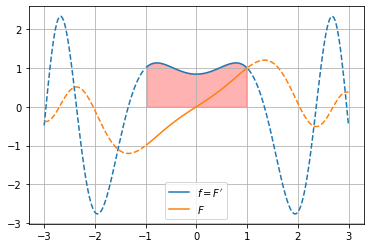
\includegraphics[scale = 0.7]{figures/reimann-integral-001.png}
        \caption{}
        \label{fig:1}
    \end{figure}

    \par Now, we want to compute the integral of $f$ on $[-1, 1]$, i.e., $\int_{-1}^1 f(x) \; \mathrm{d}x$. Applying Theorem~\ref{thm:45}, we have 
    \begin{align*}
        \int_{-1}^1 f(x) \; \mathrm{d}x
        = F(1-) - F(-1+)
        = 1 - (-1)
        =2
    \end{align*}

\end{example}

\begin{exercise} \label{ex:1}
    Let $f$ be given by 
    \begin{align*}
        f(x)
        = \frac{(1+x^2)\sin(1-x^2) - 2x^2(1-x^2)\cos(1-x^2)}{(1-x^2)^2}
        \quad x \in (-1, 1)
    \end{align*}
    Show that $f(-1+)$ and $f(1-)$ both exist, and 
    \begin{align*}
        f(-1+) = f(1-) = 1
    \end{align*}
\end{exercise}

\begin{solution}
    % TODO
\end{solution}

%------------------------------

\begin{theorem} \label{thm:46}
    Suppose $f \in \mathfrak{R}$ and $\alpha$ is continuous on $[a, b]$. Suppose further $\alpha^\prime$ exists and $\alpha^\prime \in \mathfrak{R}$ on $[a, b]$. Then $f \in \mathfrak{R}(\alpha)$ and $f \alpha^\prime \in \mathfrak{R}$ on $[a, b]$. In this case,
    \begin{align}
        \int_a^b f(x) \; \mathrm{d}\alpha(x)
        = \int_a^b f(x) \alpha^\prime(x) \; \mathrm{d}x
        \label{eq:111}
    \end{align}
\end{theorem}

\begin{remark}
    Note that the requirement of $\alpha$ being continuous is actually redundant since we assume that $\alpha^\prime$ exists on $[a, b]$. 
\end{remark}

\begin{proof}
    Since $f, \alpha^\prime \in \mathfrak{R}$, it follows from Theorem~\ref{thm:39} that their product is also integrable, i.e., $f \alpha^\prime \in \mathfrak{R}$. Theorem~\ref{thm:43} tells us we may put $\alpha^\prime$ into the integrator in the sense that 
    \begin{align}
        \int_a^b f(x) \alpha^\prime(x) \; \mathrm{d}x
        = \int_a^b f(x) \; \mathrm{d} A(x)
        \label{eq:108}
    \end{align}
    where 
    \begin{align*}
        A(x) = \int_a^x \alpha^\prime(t) \; \mathrm{d}t
    \end{align*}

    \par But we know from Theorem~\ref{thm:45} that
    \begin{align*}
        \alpha(x) - \alpha(a) = \int_a^x \alpha^\prime(t) \; \mathrm{d}t
    \end{align*}
    which implies 
    \begin{align*}
        A(x) = \alpha(x) - \alpha(a)
    \end{align*}
    Then \eqref{eq:108} reduces to 
    \begin{align}
        \int_a^b f(x) \alpha^\prime(x) \; \mathrm{d}x
        = \int_a^b f(x) \; \mathrm{d} (\alpha(x) - \alpha(a))
        \label{eq:109}
    \end{align}

    \par Note that $\alpha(a)$ is just a constant, and hence $f \in \mathfrak{R}(\alpha(a))$ and $\int_a^b f (x) \; \mathrm{d} \alpha(a) = 0$. Due to the linear property (Theorem~\ref{thm:35}) of the integrals, we have 
    \begin{align}
        \int_a^b f(x) \; \mathrm{d} (\alpha(x) - \alpha(a))
        = \int_a^b f(x) \; \mathrm{d} \alpha(x) 
        - \int_a^b f(x) \; \mathrm{d} \alpha(a)
        = \int_a^b f(x) \; \mathrm{d} \alpha(x)
        \label{eq:110}
    \end{align}
    Finally, \eqref{eq:111} follows from \eqref{eq:109} and \eqref{eq:110}.
\end{proof}

%------------------------------

\section{Change of Variables}

%------------------------------

\begin{theorem}
    
\end{theorem}

%------------------------------

%==============================

\chapter{Improper Integrals}

%==============================

\section{Improper Integral of the First Kind}

%------------------------------

\begin{definition}
    Suppose $f \in \mathfrak{R}$ on $[a,b]$ for all $b \geq a$ where $a$ is fixed. Define 
    \begin{align}
        \int_a^\infty f(x) \; \mathrm{d}x
        = \lim_{b \to \infty} \int_a^b f(x) \; \mathrm{d}x
        \label{eq:49}
    \end{align}
    provided that the limit exists and is \textbf{finite}. In that case, we say the integral on the left-hand side of \eqref{eq:49} \textbf{converges}. And this kind of improper integral with infinite integration limits is called the \textbf{improper integral of the first kind}. If 
    \begin{align*}
        \int_a^\infty \abs{f(x)} \; \mathrm{d}x
        = \lim_{b \to \infty} \int_a^b \abs{f(x)} \; \mathrm{d}x
        < \infty
    \end{align*}
    the integral $\int_a^\infty f(x) \; \mathrm{d}x$ is said to converge \textbf{absolutely}.
\end{definition}

%------------------------------

\begin{theorem}
    Suppose that $f \in \mathfrak{R}$ on $[a,b]$ for all $b \geq a$, and $f \geq 0$ on $[a, \infty)$. Let $F(b) = \int_a^b f(x) \; \mathrm{d}x$. Then $\int_a^\infty f(x) \; \mathrm{d}x$ converges if and only if $F(b)$ is bounded on $[a, \infty)$.
\end{theorem}

\begin{proof}
    Assume first $\int_a^\infty f(x) \; \mathrm{d}x$ converges, then $F(\infty) < \infty$. $F$ increases monotonically since $f \geq 0$. It follows that $F(b) \leq F(\infty) < \infty$, hence bounded. Conversely, if $F(b)$ is bounded on $[a, \infty)$, then by Proposition~\ref{pro:2}, $F(\infty)$ exists, i.e., $\int_a^\infty f(x) \; \mathrm{d}x$ converges since $F$ is increasing.
\end{proof}

%------------------------------

\begin{theorem}[Comparison Test] \label{thm:25}
    Suppose that $f, g \in \mathfrak{R}$ on $[a, b]$ for all $b \geq a$, and $f$ and $g$ satisfy the following inequality for sufficiently large $x$:
    \begin{align*}
        0 \leq f(x) \leq g(x)
        \quad \forall x > c
    \end{align*}
    where $c$ is a constant. Then we have 
    \begin{enumerate}
        \item $\int_a^\infty f(x) \; \mathrm{d}x$ converges if $\int_a^\infty g(x) \; \mathrm{d}x$ converges.
        \item $\int_a^\infty g(x) \; \mathrm{d}x$ diverges if $\int_a^\infty f(x) \; \mathrm{d}x$ diverges.
    \end{enumerate}
\end{theorem}

\begin{proof}
    % TODO
\end{proof}

%------------------------------

\begin{theorem}[Ratio Test]
    Suppose that $f, g \in \mathfrak{R}$ on $[a, b]$ for all $b \geq a$, and $g(x) > 0$ for sufficiently large $x$. Let $l$ be the limit of ratio of $f(x)$ to $g(x)$, i.e., 
    \begin{align*}
        \lim_{x \to \infty} \frac{f(x)}{g(x)} = l
    \end{align*}
    We have the following:
    \begin{enumerate}
        \item If $0 < l < \infty$, then $\int_a^\infty f(x) \; \mathrm{d}x$ and $\int_a^\infty g(x) \; \mathrm{d}x$ both converge or both diverge. In other words, $\int_a^\infty f(x) \; \mathrm{d}x$ converges if and only if $\int_a^\infty g(x) \; \mathrm{d}x$ converges.
        \item If $l = 0$, then $\int_a^\infty f(x) \; \mathrm{d}x$ converges if $\int_a^\infty g(x) \; \mathrm{d}x$ converges.
        \item If $l = \infty$, then $\int_a^\infty f(x) \; \mathrm{d}x$ diverges if $\int_a^\infty g(x) \; \mathrm{d}x$ diverges.
    \end{enumerate}
\end{theorem}

\begin{remark}
    Note that all the conclusions are about $\int_a^\infty f(x) \; \mathrm{d}x$. Indeed, the test is used to determine the convergence of $\int_a^\infty f(x) \; \mathrm{d}x$ based on the knowledge of convergence of $\int_a^\infty g(x) \; \mathrm{d}x$
\end{remark}

\begin{proof}
    (Proof of 1) Choose $0 < \varepsilon < l$. Then there exists $c > a$ such that 
    \begin{align*}
        \abs{\frac{f(x)}{g(x)} - l} < \varepsilon
        \quad \forall x > c
    \end{align*}
    and $g(x) > 0 \; \forall x > c$. It follows that 
    \begin{align*}
        (l - \varepsilon) g(x) < f(x) < (l + \varepsilon) g(x)
        \quad \forall x > c
    \end{align*}
    By the Comparison Test (Theorem~\ref{thm:25}), 
    \begin{align*}
        0 < (l - \varepsilon) g(x) < f(x)
        \quad \forall x > c
    \end{align*}
    implies that $\int_a^\infty g(x) \; \mathrm{d}x$ converges if $\int_a^\infty f(x) \; \mathrm{d}x$ converges. Similarly,
    \begin{align*}
        0 \leq f(x) < (l + \varepsilon) g(x)
        \quad \forall x > c
    \end{align*}
    implies that $\int_a^\infty f(x) \; \mathrm{d}x$ converges if $\int_a^\infty g(x) \; \mathrm{d}x$ converges.

    \par (Proof of 2) Choose a positive number $\varepsilon > 0$. There exists $c > a$ such that 
    \begin{align*}
        \abs{\frac{f(x)}{g(x)}} < \varepsilon
        \quad \forall x > c
    \end{align*}
    and $g(x) > 0 \; \forall x > c$. Rearranging the above inequality, we obtain
    \begin{align*}
        0 \leq f(x) <  \varepsilon g(x)
    \end{align*}
    Thus, it follows from the Comparison Test that $\int_a^\infty f(x) \; \mathrm{d}x$ converges if $\int_a^\infty g(x) \; \mathrm{d}x$ converges. 

    \par (Proof of 3) Choose a positive number $M > 0$. By the definition of infinite limits, there exists $c > a$ such that 
    \begin{align*}
        \frac{f(x)}{g(x)} > M
        \quad \forall x > c
    \end{align*}
    and $g(x) > 0 \; \forall x > c$. It follows that 
    \begin{align*}
        f(x) > M g(x) > 0
        \quad \forall x > c
    \end{align*}
    Then $\int_a^\infty f(x) \; \mathrm{d}x$ diverges if $\int_a^\infty g(x) \; \mathrm{d}x$ diverges.
\end{proof}

%------------------------------

\begin{theorem}[Integral Test] \label{thm:22}
    Suppose that $f \geq 0$ and $f$ decreases monotonically on $[1, \infty)$. Then 
    \begin{align*}
        \int_1^\infty f(x) \; \mathrm{d}x
    \end{align*}
    converges if and only if 
    \begin{align*}
        \sum_{n=1}^\infty f(n)
    \end{align*}
    converges.
\end{theorem}

\begin{proof}
    % TODO
\end{proof}

%------------------------------

\section{Dirichlet's Test and Abel's Test for Improper Integrals}

%------------------------------

%==============================

\chapter{Sequences and Series of Functions}

\par In the introduction of pointwise and uniform convergence of functions, we confine ourselves to complex-valued functions whose domains lie in \textit{metric spaces}.

%==============================

\section{Discussion of Main Problem}

%------------------------------

\begin{definition} \label{def:1}
    Let $\{f_n\}$ be a sequence of functions on $E$. If for any $x \in E$, the limit of the numerical sequence $\{f_n(x)\}$ exists, then the function defined by
    \begin{align*}
        f(x) = \lim_{n \to \infty} f_n(x)
    \end{align*}
    is called the \textbf{limit} of $\{f_n\}$.
\end{definition}

\par We say $f_n$ converges \textit{pointwise} to $f$ if $f_n$ only satisfies the above definition. There is a stronger version of convergence called uniform convergence, which will be introduced later.

\par If we regard $\{\sum_{m=0}^{n} f_m\}_n$ as a sequence of partial sums, we can define the \textit{sum} of series of functions $\sum f_n$ as the \textit{limit} of the sequence of partial sums.

\begin{definition} \label{def:2}
    If $\sum f_n(x)$ converges (i.e., the limit of the partial sum exists) for each $x \in E$, and if we define 
    \begin{align*}
        f(x) = \sum_{n=0}^{\infty} f_n(x)
    \end{align*} 
    then $f$ is called the \textbf{sum} of series $\sum f_n$.
\end{definition}

%------------------------------

\section{Uniform Convergence}

%------------------------------

\begin{definition} \label{def:3}
    We say a sequence of functions $\{f_n\}$ converges \textbf{uniformly} on $E$ to a function $f$ if for an arbitrary $\varepsilon > 0$, there exists $N \in \Ns$ such that $n \geq N$ implies 
    \begin{align*}
        \abs{f_n(x) - f(x)} < \varepsilon
    \end{align*}
    for all $x \in E$.
\end{definition}

%------------------------------

\par An analogous definition above exists for the series of functions.

\begin{definition} \label{def:4}
    We say a series of functions $\sum f_n$ converges \textbf{uniformly} on $E$ to a function $f$ if for an arbitrary $\varepsilon > 0$, there exists $N \in \Ns$ such that $n \geq N$ implies 
    \begin{align*}
        \abs{\sum_{m=0}^{n} f_m(x) - f(x)} < \varepsilon
    \end{align*}
    for all $x \in E$.
\end{definition}

%------------------------------

\par The Cauchy criterion for uniform convergence is as follows.

\begin{theorem}[Cauchy Criterion] \label{thm:6}
    The sequence of functions $\left\{f_n\right\}$, defined on $E$, converges uniformly if and only if for any $\varepsilon > 0$, there exists $N \in \Ns$ such that $m, n \geq N$, $x \in E$ implies 
    \begin{align*}
        \abs{f_n(x) - f_m(x)} < \varepsilon
    \end{align*}
\end{theorem}

\begin{proof}
    % TODO
\end{proof}

%------------------------------

\par The following theorem is another criterion for uniform convergence, which provides us with insight into measuring the distance between two functions.

\begin{theorem} \label{thm:8}
    Suppose the sequence of functions $\left\{f_n\right\}$ converges pointwise to $f$ on $E$. Put 
    \begin{align*}
        M_n = \sup_{x \in E} \abs{f_n(x) - f(x)}
    \end{align*}
    Then $f_n \to f$ uniformly if and only if $\lim_{n \to \infty} M_n = 0$.
\end{theorem}

\begin{remark}
    $\sup_{x \in E} \abs{f_n(x) - f(x)}$ actually defines a distance function $d(f_n, f)$, which we will discuss in more details later.
\end{remark}

\begin{proof}
    % TODO
\end{proof}

%------------------------------

\par For series, there is a very convenient test called Weierstrass's M-Test for uniform convergence.

\begin{theorem}[Weierstrass's M-Test] \label{thm:14}
    Let $\left\{f_n\right\}$ be a sequence of functions defined on $E$, and suppose 
    \begin{align*}
        \abs{f_n(x)} \leq M_n \quad \forall x \in E
    \end{align*}
    Then $\sum f_n$ converges uniformly on $E$ if $\sum M_n$ converges.
\end{theorem}

\begin{proof}
    % TODO
\end{proof}

%------------------------------

\section{Uniform Convergence and Continuity}

%------------------------------

\par The uniform convergence of functions allows us to interchange change limits.

\begin{theorem} \label{thm:7}
    Suppose $f_n \to f$ uniformly on $E \subset X$ where $X$ is a metric space. Let $x$ be a limit point of $E$. If the limit $A_n := \lim_{t \to x} f_n(t)$ exists, then $\left\{A_n\right\}$ converges and
    \begin{align*}
        \lim_{t \to x} f(t) = \lim_{n \to \infty} A_n
    \end{align*}
    In other words, 
    \begin{align}
        \lim_{t \to x} \lim_{n \to \infty} f_n(t)
        = \lim_{n \to \infty} \lim_{t \to x} f_n(t)
        \label{eq:11}
    \end{align}
\end{theorem}

\begin{remark}
    One way to remember this theorem is that if the \textit{inner} limits on both sides of \eqref{eq:11} exist, then the \textit{outer} limits also exist and are equal to each other.
\end{remark}

\begin{proof}
    We first prove that $\left\{A_n\right\}$ converges. Given $\varepsilon > 0$, since $\left\{f_n\right\}$ converges uniformly, there exists $N \in \Ns$ such that $n, m \geq N$ implies that 
    \begin{align}
        \abs{f_n(t) - f_m(t)} < \varepsilon \quad 
        \forall t \in E
        \label{eq:7}
    \end{align}
    due to Theorem~\ref{thm:6}. Because the limits $\lim_{t \to x} f_n(t)$ and $\lim_{t \to x} f_m(t)$ both exist, the limit of the left-hand side of \eqref{eq:7} also exists as $t \to x$. Letting $t \to x$, we have
    \begin{align*}
        \abs{A_n - A_m}
        = \abs{\lim_{t \to x} f_n(t) - \lim_{t \to x} f_m(t)}
        = \lim_{t \to x} \abs{f_n(t) - f_m(t)} 
        \leq \varepsilon
    \end{align*}
    Therefore, $\left\{A_n\right\}$ indeed converges due to the Cauchy criterion for convergence of sequences.
    
    \par We now show that the limit of $f(t)$ exists as $t \to x$, and it equals $A := \lim_{n \to \infty} A_n$. Let $\varepsilon > 0$ be arbitrary. Since $f_n \to f$ uniformly on $E$, there exists $N_1 \in \Ns$ such that 
    \begin{align}
        \abs{f(t) - f_n(t)} < \frac{\varepsilon}{3} \quad \forall n \geq N_1, \; \forall t \in E
        \label{eq:8}
    \end{align}
    And since $f_n(t) \to A_n$ as $t \to x$, there exists a neighborhood $V$ of $x$ such that 
    \begin{align}
        \abs{f_n(t) - A_n} < \frac{\varepsilon}{3} \quad \forall t \in V \cap E
        \label{eq:9}
    \end{align}
    Moreover, because we have proved $\lim_{n \to \infty} A_n = A$, there exists $N_2 \in Ns$ such that
    \begin{align}
        \abs{A_n - A} < \frac{\varepsilon}{3} \quad \forall n \geq N_2
        \label{eq:10}
    \end{align}
    Let $N = \max\{N_1, N_2\}$. Suppose $t \in V \cap E$ and $n \geq N$, by \eqref{eq:8}, \eqref{eq:9} and \eqref{eq:10}, we have
    \begin{align*}
        \abs{f(t) - A}
        \leq \abs{f(t) - f_n(t)}
        + \abs{f_n(t) - A_n}
        + \abs{A_n - A} 
        < \frac{\varepsilon}{3} + \frac{\varepsilon}{3} + \frac{\varepsilon}{3}
        = \varepsilon
    \end{align*}
    Therefore, $\lim_{t \to x} f(t) = A$.
\end{proof}

%------------------------------

\par An immediate corollary to Theorem~\ref{thm:7} is that if a sequence of continuous functions converges uniformly to some function, then that limit function is also continuous.

\begin{theorem} \label{thm:11}
    Let $\left\{f_n\right\}$ be a sequence of continuous functions on $E$. If $f_n \to f$ uniformly on $E$, then $f$ is also continuous.
\end{theorem}

\begin{remark}
    However, the converse of this theorem is not true in general. That is, if $f$ is continuous it is not necessary that $f_n \to f$ uniformly. Or in other words, it is possible in some cases that $f_n \to f$ only pointwise, and $f$ is still continuous. The following example is one such case.
\end{remark}

\begin{example} \label{eg:1}
    Let
    \begin{align*}
        f_n(x) = n^2 x (1 - x^2)^n
    \end{align*}
    where $0 \leq x \leq 1$ and $n \in \Ns$. Note that 
    \begin{align*}
        f(x) = \lim_{n \to \infty} f_n(x) = 0
    \end{align*}
    All $f_n$'s are continuous and $f$ is of course continuous since it is a constant function. But $\left\{f_n\right\}$ does not converge to $f$ uniformly on $[0,1]$ due to Theorem~\ref{thm:8}. To see this, one can obtain
    \begin{align*}
        M_n = \sup_{x \in [0,1]} f_n(x)
        = \frac{n^2}{\sqrt{1 + 2n}} \left(1 - \frac{1}{1+2n}\right)^n 
    \end{align*}
    by computing the critical points of $f_n(x)$. Note that 
    \begin{align*}
        \lim_{n \to \infty} \left(1 - \frac{1}{1+2n}\right)^n
        = \lim_{n \to \infty} \sqrt{\frac{1}{\left(1 + \frac{1}{2n}\right)^{2n}}}
        = \frac{1}{\sqrt{e}}
    \end{align*}
    But $\frac{n^2}{\sqrt{1 + 2n}} \to \infty$ as $n \to \infty$. Therefore, $\lim_{n \to \infty} M_n = \infty$. Since $M_n$ does not converge to $0$, Theorem~\ref{thm:8} implies that $\left\{f_n\right\}$ does not converge to $f$ uniformly.
\end{example}

%------------------------------

\begin{proof}
    Let a sequence $\left\{x_n\right\}_{n \in \N}$ be given by 
    \begin{align*}
        x_0 &= 0 \\ 
        x_n &= \frac{1}{n} \quad n \geq 1
    \end{align*}
    Let $E$ be the set consisting of terms of this sequence, i.e, 
    \begin{align*}
        E = \set{x \in \R}{\exists n \in \N, \; x_n = x} = \left\{0\right\} \cup \set{\frac{1}{n}}{n \in \Ns}
    \end{align*}
    It is clear that $\lim_{n \infty} x_n = x_0$, and $x_n \to x_0$ if and only if $n \to \infty$. We now define a sequence of functions $\left\{f_i\right\}_{i \in \Ns}$ on $E$ by specifying the function value at each point:
    \begin{align*}
        f_i(x_0) &:= \sum_{j=1}^\infty a_{ij} \\ 
        f_i(x_n) &:= \sum_{j=1}^n a_{ij} 
        \quad n \geq 1
    \end{align*}
    And then let function $g$ be defined by 
    \begin{align*}
        g(x) := \sum_{i=1}^\infty f_i(x)
    \end{align*}

    \par We need to verify that functions $f_i$'s and $g$ are all well-defined. 
    $f_i(x_n)$ is well-defined since it is just a finite sum of complex numbers. In the conditions of this theorem, we require that $\sum_{j=1}^\infty a_{ij}$ converges absolutely, hence the well-definedness of $f(x_0)$.
    For function $g$, we note that 
    \begin{align}
        f_i(x) 
        \leq \abs{f_i(x)}
        \leq \sum_{j=1}^\infty \abs{a_{ij}}
        = b_i < \infty
        \label{eq:17}
    \end{align}
    Since $\sum b_i$ converges, we know $\sum \abs{f_i(x)}$ also converges by the Comparison Test. Therefore, $\sum f_i(x)$ converges (absolutely), and hence $g(x)$ is well-defined. Moreover, \eqref{eq:17} implies that $\sum f_i(x)$ converges \textit{uniformly} to $g(x)$ by Weierstrass's M-Test (Theorem~\ref{thm:14}).

    \par In the following, we show that $f_i$ is \textit{continuous} at $x_0$. Given $\varepsilon > 0$, there exists $N \in \Ns$ such that $n \geq N$ implies 
    \begin{align*}
        \abs{f_i(x_n) - f_i(x_0)}= \abs{\sum_{j=1}^n a_{ij} - \sum_{j=1}^\infty a_{ij}} < \varepsilon
    \end{align*}
    Choose a positive number $\delta < \frac{1}{N}$, and then let $\abs{x-x_0} < \delta$ ($x \in E$). Since $x \in E$, $x = x_n$ for some $n \in \N$. Then, by the definition of $x_n$, it is clear $n > N$. It follows that if $\abs{x - x_0} < \delta$, we have 
    \begin{align*}
        \abs{f_i(x_n) - f_i(x_0)} < \varepsilon
    \end{align*}
    since $n > N$. Therefore, $f_i$ is indeed continuous at $x_0$.

    \par Recall $\sum f_i(x)$ converges uniformly to $g(x)$. It follows that $g$ is also continuous at $x_0$ due to Theorem~\ref{thm:7}. Then, we have
    \begin{align*}
        g(x_0) = \lim_{x \to x_0} g(x)
        = \lim_{n \to \infty} g(x_n)
    \end{align*}
    The last equation (converting limit of function limit to limit of sequence) holds because $\left\{x_n\right\}$ is indeed a sequence that converges to $x_0$. It then follows that 
    \begin{align*}
        g(x_0) = g(x)
        = \lim_{n \to \infty} g(x_n)
        &= \lim_{n \to \infty} \sum_{i=1}^\infty f_i(x_n) \\
        &= \lim_{n \to \infty} \sum_{i=1}^\infty \sum_{j=1}^n a_{ij} \\ 
        &= \lim_{n \to \infty} \sum_{j=1}^n \sum_{i=1}^\infty a_{ij} \\
        &= \sum_{j=1}^\infty \sum_{i=1}^\infty a_{ij}
    \end{align*}
    Note that the reason why we have 
    \begin{align*}
        \sum_{i=1}^\infty \sum_{j=1}^n a_{ij}
        = \sum_{j=1}^n \sum_{i=1}^\infty a_{ij}
    \end{align*}
    is that $\sum_{i=1}^\infty a_{ij}$ converges.
    In summary, on the one hand, we have shown 
    \begin{align}
        g(x_0) = \sum_{j=1}^\infty \sum_{i=1}^\infty a_{ij}
        \label{eq:18}
    \end{align}
    On the other hand, by definition, 
    \begin{align}
        g(x_0) = \sum_{i=1}^\infty f_i(x_0)
        = \sum_{i=1}^\infty \sum_{j=1}^\infty a_{ij}
        \label{eq:19}
    \end{align}
    We complete the proof by equating the right-hand sides of \eqref{eq:18} and \eqref{eq:19}.
\end{proof}

%------------------------------

\begin{theorem}
    Suppose $K$ is a compact set, and 
    \begin{enumerate}
        \item $\left\{f_n\right\}$ is a sequence of continuous functions on $K$
        \item $f_n \to f$ pointwise where $f$ is also continuous
        \item $f_n(x) \geq f_{n+1}(x)$ for all $x \in K$, $n \in \Ns$
    \end{enumerate}
    Then $f_n \to f$ uniformly on $K$.
\end{theorem}

\begin{proof}
    Let $g_n(x) := f_n(x) - f(x)$. It is clear that $g_n(x) \geq g_{n+1}(x) \geq 0$ and $g_n \to g \equiv 0$ pointwise. Given $\varepsilon > 0$. Define set
    \begin{align*}
        K_n := g_n^{-1}[\varepsilon, \infty)
    \end{align*}
    Since, $g_n$ is continuous and $[\varepsilon, \infty)$ is closed in $\R$, it follows that $K_n$ is a compact subset. Consider the intersection $\bigcap_{n \in \Ns} K_n$. Because $g_n \geq g_{n+1}$, we have
    \begin{align*}
        K_{n} \supset K_{n+1}
    \end{align*}
    We now claim that $\bigcap_{n \in \Ns} K_n = \emptyset$. To see this, we assume $x \in \bigcap_{n \in \Ns} K_n$, which then implies $g_n(x) \geq \varepsilon \; \forall n \in \Ns$. This leads to a contradiction since $g_n \to g \equiv 0$. Having that $\bigcap_{n \in \Ns} K_n = \emptyset$, by Theorem~\ref{thm:10}, it follows that there exists some finite subset $J \subset \Ns$ such that $\bigcap_{n \in J} K_n = \emptyset$. Suppose the largest number in $J$ is $N$, then we have
    \begin{align*}
        K_N = \bigcap_{n \in J} K_n = \emptyset 
    \end{align*}
    since $K_n \supset K_{n+1}$. This further implies that
    \begin{align}
        K_N = \emptyset \quad \forall n \geq N
        \label{eq:12}
    \end{align}
    It then follows from \eqref{eq:12} and the definition of $K_n$ that 
    \begin{align*}
        0 \leq g_n(x) < \varepsilon \quad \forall n \geq N, \; \forall x \in K
    \end{align*}
    Therefore, $g_n \to 0$ uniformly, i.e., $f_n \to f$ uniformly.
\end{proof}

\par The compactness is necessary. Consider the following example.

\begin{example}
    Let $f_n(x) = \frac{1}{nx}$ where $x \in (0,1)$, which is not a compact set in $\R$. Note that $f_n \to 0$ pointwise, all functions are continuous and $f_n(x) > f_{n+1}(x)$. But clearly $\left\{f_n\right\}$ does not converge to $0$ uniformly on $(0,1)$.
\end{example}

\par The condition that $f_n(x) \geq f_{n+1}(x)$ is also crucial to this theorem. To illustrate this, we reconsider example~\ref{eg:1}.

\begin{example}
    Let $f_n$ be the same function in example~\ref{eg:1}. The domain $[0,1]$ is compact and $f_n$ is continuous. We have already seen that $\left\{f_n\right\}$ does not converge to $0$ uniformly on $[0,1]$. What goes wrong is that $\left\{f_n\right\}$ fails to satisfy $f_n(x) \geq f_{n+1}(x)$ (for \textit{infinitely} many $n$). To see this, we evaluate $f_n$ and $f_{n+1}$ at the point $x = \frac{1}{\sqrt{2n+3}}$ (the maximum point of $f_{n+1}$). We have 
    \begin{align*}
        \frac{f_{n}(1/\sqrt{2n+3})}{f_{n+1}(1/\sqrt{2n+3})}
        = \frac{n^2(2n+3)}{2(n+1)^3}
        = \frac{2n^3 + 3n^2}{2n^3 + 6n^2 + 6n + 2}
        < 1
    \end{align*}
    Therefore,
    \begin{align*}
        f_{n}(1/\sqrt{2n+3}) < f_{n+1}(1/\sqrt{2n+3}) 
        \quad \forall n \in \Ns
    \end{align*}
\end{example}

%------------------------------

\par If we collect a certain kind of functions in a set, we can then interpret uniform convergence of functions simply as sequential convergence. In this case, each term of the sequence is not some number but a \textit{function}.

\begin{definition}
    Let $X$ be a metric space. $\mathscr{C}(X)$ will denote the set consisting of all complex-valued, bounded and continuous functions with domain $X$.
\end{definition}

%------------------------------

\par Next, to make $\mathscr{C}(X)$ a metric space, we need to define a distance function. We do so by first defining norms.

\begin{definition} \label{def:5}
    The norm on $\mathscr{C}(X)$ is given by the supremum norm of each function $f \in \mathscr{C}(X)$, i.e.,  
    \begin{align*}
        \norm{f} := \sup_{x \in X}\abs{f(x)}
    \end{align*}
\end{definition}

\begin{remark}
    We need to verify that Definition~\ref{def:5} indeed defines a norm. It is clearly positive definite, and 
    \begin{align*}
        \norm{\alpha f} 
        = \sup_{x \in X}\abs{\alpha f(x)}
        = \abs{\alpha} \sup_{x \in X} \abs{f(x)}
        = \abs{\alpha} \norm{f}
    \end{align*}
    where $\alpha \in \C$. Moreover, 
    \begin{align*}
        \norm{f+g}
        = \sup_{x \in X} \abs{f(x) + g(x)}
        \leq \sup_{x \in X} (\abs{f(x)} + \abs{g(x)})
        \leq \sup_{x \in X}\abs{f(x)} + \sup_{x \in X}\abs{g(x)}
        = \norm{f} + \norm{g}
    \end{align*}
\end{remark}

%------------------------------

\par The distance function on $\mathscr{C}(X)$ is defined as the norm of the difference between two functions.

\begin{definition}
    The distance function on $\mathscr{C}(X)$ is given by 
    \begin{align*}
        d(f, g) := \norm{f - g}
    \end{align*}
    where $f, g \in \mathscr{C}(X)$ and $\norm{\cdot}$ is the norm on $\mathscr{C}(X)$.
\end{definition}

\begin{remark}
    With the properties of norms, it is easy to verify that the distance function is well-defined.
\end{remark}

%------------------------------

\par Associate with a distance function, we are now able to call $\mathscr{C}(X)$ a metric space. Even better, $\mathscr{C}(X)$ is a \textit{complete} metric space, which we shall prove below.

\begin{theorem}
    $\mathscr{C}(X)$ is a \textbf{complete} metric space.
\end{theorem}

\begin{remark}
    Let $\left\{f_n\right\}$ be a sequence in $\mathscr{C}(X)$. Then $f_n \to f$ uniformly on $X$ is equivalent to that $\left\{f_n\right\}$ converges to $f$. Moreover, $f \in \mathscr{C}(X)$.
\end{remark}

\begin{proof}
    Let $\left\{f_n\right\}$ be a Cauchy sequence in $\mathscr{C}(X)$. Then for given $\varepsilon > 0$, there exists $N \in \Ns$ such that $n, m \geq N$ implies 
    \begin{align*}
        \sup_{x \in X}\abs{f_n(x) - f_m(x)}= d(f_n, f_m) < \varepsilon
    \end{align*}
    By Theorem~\ref{thm:6}, there exists some function $f$ such that $f_n \to f$ uniformly on $f$. (Note that $f$ is not necessary in $\mathscr{C}(X)$ for now. That is exactly what we need to prove.) We intend to show that $f \in \mathscr{C}(X)$. By Theorem~\ref{thm:11}, $f$ is continuous since all $f_n$'s are continuous. We also need to show that $f$ is bounded. By Theorem~\ref{thm:8}, we have 
    \begin{align*}
        \sup_{x \in X} \abs{f(x) - f_N(x)} < 1
    \end{align*}
    for some $N \in \Ns$. And $\sup_{x \in X}\abs{f_N(x)} < M$ for some $M > 0$ since $f_N$ is bounded. It then follows that 
    \begin{align*}
        \sup_{x \in X} \abs{f(x)}
        \leq \sup_{x \in X} \abs{f(x) - f_N(x)} + \sup_{x \in X}\abs{f_N(x)}
        < 1 + M
    \end{align*}
    Therefore, $f$ is indeed bounded. Hence, $f \in \mathscr{C}(X)$ since we have proved $f$ is bounded and continuous (of course, $f$ is also complex-valued). As Theorem~\ref{thm:8} states,
    \begin{align*}
        \lim_{n \to \infty} d(f_n, f) = 0
    \end{align*}
    with $f \in \mathscr{C}(X)$, we may conclude that $\mathscr{C}(X)$ is a complete metric space.
\end{proof}

%------------------------------

\section{Uniform Convergence and Integration}

%------------------------------

%------------------------------

\section{Uniform Convergence and Differentiation}

%------------------------------

\begin{theorem}
    Let $\left\{f_n\right\}$ be a sequence of differentiable functions defined on $[a,b]$. Suppose that the numerical sequence $\left\{f_n(x_0)\right\}$ converges where $x_0 \in [a,b]$, and the sequence $\left\{f_n^\prime\right\}$ converges uniformly on $[a,b]$. Then $\left\{f_n\right\}$ converges uniformly to some function $f$ on $[a, b]$. Moreover, $f$ is differentiable on $[a, b]$, the limit of $\left\{f_n^\prime(x)\right\}$ exists for each $x$, and
    \begin{align}
        f^\prime(x) = \lim_{n \to \infty} f_n^\prime(x)
        \label{eq:16}
    \end{align}
    In other words, we can interchange differentiation and limit, i.e., 
    \begin{align*}
        \frac{\mathrm{d}}{\mathrm{d} x} \lim_{n \to \infty} f_n(x)
        = \lim_{n \to \infty} \frac{\mathrm{d}}{\mathrm{d} x} f_n(x)
    \end{align*}
\end{theorem}

\begin{remark}
    Pay attention to the conditions of this theorem. The reason that we do not assume the uniform convergence of $\left\{f_n\right\}$ directly is that it is not sufficient to guarantee the interchange of differentiation and limit. Therefore, stronger conditions are needed. We assume the uniform convergence of the sequence of derivatives $\left\{f_n^\prime\right\}$, and we also require that $f_n$ converges at one point. And in fact, the uniform convergence of $\left\{f_n\right\}$ can be derived based on that.
\end{remark}

\begin{proof}
    The first thing we need to show is that $\left\{f_n\right\}$ converges uniformly. Given $\varepsilon > 0$, there exists some $N_1 \in \Ns$ such that $n, m \geq N_1$ implies
    \begin{align}
        \abs{f_n(x_0) - f_m(x_0)} < \frac{\varepsilon}{2}
        \label{eq:13}
    \end{align}
    since $\left\{f_n(x_0)\right\}$ converges. Furthermore, because $\left\{f_n^\prime\right\}$ converges uniformly, there exists some $N_2 \in \Ns$ such that $n, m \geq N_2$ implies
    \begin{align}
        \abs{f_n^\prime(x) - f_m^\prime(x)}
        < \frac{\varepsilon}{2(b-a)}
        \quad \forall x \in [a, b]
        \label{eq:14}
    \end{align}
    Let $N = \max\{N_1, N_2\}$ and $n, m \geq N$. If we regard function $f_n(x) - f_m(x)$ as a whole, then by the Mean Value Theorem, we have 
    \begin{align}
        \left(f_n(x) - f_m(x)\right)
        - \left(f_n(x_0) - f_m(x_0)\right)
        = (x - x_0) \left(f_n^\prime(\xi_x) - f_m^\prime(\xi_x)\right)
        \label{eq:15}
    \end{align}
    for some $\xi_x$ (depending on $x$) in between $x$ and $x_0$. Taking into consideration \eqref{eq:13}, \eqref{eq:14} and \eqref{eq:15}, it then follows that 
    \begin{align*}
        \abs{f_n(x) - f_m(x)}
        &\leq \abs{f_n(x_0) - f_m(x_0)}
        + \abs{x-x_0} \abs{f_n^\prime(\xi_x) - f_m^\prime(\xi_x)} \\ 
        &< \frac{\varepsilon}{2} 
        + (b-a) \frac{\varepsilon}{2(b-a)} \\ 
        &= \varepsilon \quad \forall x \in [a, b]
    \end{align*}
    Therefore, $\left\{f_n\right\}$ converges uniformly on $[a, b]$ by Theorem~\ref{thm:6}. Let $f$ be the limit of this sequence of functions, i.e., $f(x) = \lim_{n \to \infty} f_n(x)$.

    \par We then show that $f$ is differentiable, the limit of $\left\{f_n^\prime(x)\right\}$ exists and \eqref{eq:16} holds. Fix an $x$ in $[a, b]$. Define 
    \begin{align*}
        \phi_n(t) &:= \frac{f_n(x) - f_n(t)}{x - t} \\
        \phi(t) &:= \frac{f(x) - f(t)}{x - t}
    \end{align*}
    where $t \in [a, b] \setminus \{x\}$. Let $\varepsilon > 0$ be arbitrary. By applying the same argument, we will again obtain \eqref{eq:14} and \eqref{eq:15} (with $x$ replaced by $t$ and $x_0$ replaced by $x$). It then follows from \eqref{eq:15} that 
    \begin{align*}
        \abs{\phi_n(t) - \phi_m(t)}
        = \abs{f_n^\prime(\xi_t) - f_m^\prime(\xi_t)}
    \end{align*}
    Then by letting $n, m \geq N_2$, we have
    \begin{align*}
        \abs{\phi_n(t) - \phi_m(t)}
        = \abs{f_n^\prime(\xi_t) - f_m^\prime(\xi_t)}
        < \frac{\varepsilon}{2(b-a)}
        \quad \forall t \in [a, b] \setminus \{x\}
    \end{align*}
    due to \eqref{eq:14}. Therefore, $\phi_n$ converges uniformly on $[a, b] \setminus \{x\}$. And since we have proved $f_n \to f$ as $n \to \infty$, it is clear that the limit of $\left\{\phi_n\right\}$ is $\phi$, i.e., $\phi_n \to \phi$ uniformly on $[a, b] \setminus \{x\}$. Finally, by applying Theorem~\ref{thm:7}, we have 
    \begin{align*}
        \lim_{t \to x} \phi(t)
        = \lim_{n \to \infty} \lim_{t \to x} \phi_n(t)
        = \lim_{n \to \infty} f_n^\prime(x)
    \end{align*}
    (The existence of involved limits is implied by Theorem~\ref{thm:7}.) Note that $\lim_{t \to x} \phi(t)$ is precisely the definition of $f^\prime(x)$. This completes the proof.
\end{proof}

\begin{example}
    
\end{example}

%------------------------------

%------------------------------

%==============================

\chapter{Some Special Functions}

%==============================

\section{Power Series}

\par In this section, we study the properties of power series, i.e., the function of the form 
\begin{align*}
    f(x) = \sum c_n x^n
\end{align*}
where $c_n, x \in \R$. The reason why we confine ourselves to real values is that we have only defined differentiation and integration in the real field.

%------------------------------

\begin{theorem} \label{thm:18}
    Suppose that the power series 
    \begin{align*}
        \sum_{n=0}^{\infty} c_n x^n
    \end{align*}
    converges for $\abs{x} < R$ where $c_n, x \in \R$ and $R > 0$. Define 
    \begin{align*}
        f(x) = \sum_{n=0}^{\infty} c_n x^n
    \end{align*}
    Then $f$ converges uniformly on $[-R + \varepsilon, R - \varepsilon]$ for any $\varepsilon \in (0, R)$. Moreover, $f$ is differentiable in the interval $(-R, R)$, and 
    \begin{align*}
        f^\prime(x) = \sum_{n=1}^{\infty} n c_n x^{n-1}
    \end{align*}
\end{theorem}

\begin{proof}
    % TODO
\end{proof}

%------------------------------

\begin{corollary} \label{cor:2}
    The power series $f(x) = \sum_{n=0}^\infty c_n x^n$ (which converges for $x \in (-R, R)$, $R > 0$) has derivatives of all orders in $(-R, R)$, which are given by 
    \begin{align}
        f^{(k)}(x)
        = \sum_{n=k}^\infty \left( \prod_{i=0}^{k-1}(n-i)\right) c_n x^{n-k}
        = \sum_{n=k}^\infty n(n-1) \cdots (n-k+1) c_n x^{n-k}
        \label{eq:33}
    \end{align}
    where $k \in \N$ ($f^{(0)}$ means $f$). Furthermore, putting $x = 0$ in \eqref{eq:33}, we obtain the equality
    \begin{align}
        c_n = \frac{f^{(n)}(0)}{n!}
        \label{eq:34}
    \end{align}
\end{corollary}

%------------------------------

\subsection{Negative Binomial Theorem}

\par It is well known that 
\begin{align*}
    \frac{1}{1-x} = \sum_{k=0}^\infty x^k
    \quad -1 < x < 1
\end{align*}
The right-hand side is a geometric series, and we can easily compute its explicit value, which equals the left-hand side. The Negative Binomial Theorem is a generalization for it states the power series representation of the function $\frac{1}{(1-x)^n}$.

%------------------------------

\begin{theorem}[Negative Binomial Theorem] \label{thm:16} % MINE
    We have the following identity:
    \begin{align}
        \frac{1}{(1-x)^n}
        = \sum_{k=0}^\infty \binom{n+k-1}{k} x^k
        \label{eq:30}
    \end{align}
    where $x \in \R$, $\abs{x} < 1$ and $n \in \Ns$. Moreover, the power series on right-hand side of \eqref{eq:30} converges only when $\abs{x} < 1$.
\end{theorem}

\begin{proof}
    Let
    \begin{align*}
        f(x) = \frac{1}{1-x}
        \quad -1 < x < 1
    \end{align*}
    The $(n-1)$-th order of derivative of $f$ is 
    \begin{align}
        f^{(n-1)}(x) = \frac{(n-1)!}{(1-x)^{n}}
        \label{eq:40}
    \end{align}
    On the other hand, applying \eqref{eq:33} in Corollary~\ref{cor:2}, we obtain 
    \begin{align}
        f^{(n-1)}(x) = \sum_{k=n-1}^\infty k(k-1) \cdots (k-n+1) x^{k-n}
        = \sum_{k=0}^\infty (k+n-1)(k+n-2) \cdots (k+1) x^{k}
        \label{eq:41}
    \end{align}
    Comparing \eqref{eq:40} and \eqref{eq:41}, we have 
    \begin{align*}
        \frac{(n-1)!}{(1-x)^{n}}
        = \sum_{k=0}^\infty (k+n-1)(k+n-2) \cdots (k+1) x^{k}
    \end{align*}
    Therefore,
    \begin{align*}
        \frac{1}{(1-x)^{n}}
        = \sum_{k=0}^\infty \frac{(k+n-1)(k+n-2) \cdots (k+1)}{(n-1)!} x^{k}
        = \sum_{k=0}^\infty \binom{n+k-1}{k} x^{k}
    \end{align*}

    \par So far, we have shown \eqref{eq:30} indeed converges in $\abs{x} < 1$. We also need to show that it cannot converge for $\abs{x} \geq 1$. In fact, we only need to show it does not converge for $\abs{x} = 1$ due to Theorem~\ref{thm:13}. Suppose $\abs{x} = 1$. We consider the absolute value of each term of the series.
    \begin{align}
        \abs{\binom{n+k-1}{k} x^k}
        = \binom{n+k-1}{k}
        = \binom{n+k-1}{n-1}
        \label{eq:42}
    \end{align}
    Note that the combinatorial number \eqref{eq:42} will tend to $\infty$ as $k \to \infty$. Thus, series \eqref{eq:30} will of course diverge for $\abs{x} = 1$.
\end{proof}

%------------------------------

\par We note that $\frac{1}{(1-x)^n}$ is obtained by multiplying $\frac{1}{1-x}$ by itself $n-1$ times. It is tempting to multiply the power series $\sum x^k$. Hence, another strategy for proving this theorem is to compute the \textit{Cauchy Product} of these $n$ series $\sum x^k$.

\par In the alternative proof, we will need an identity from combinatorial mathematics, which is known as the Hockey-Stick Identity.

\begin{theorem}[Hockey-Stick Identity]
    We have the identity:
    \begin{align*}
        \sum_{i=r}^n \binom{i}{r} = \binom{n+1}{r+1}
    \end{align*}
\end{theorem}

\par Observe the bold numbers in Pascal's Triangle below. 

\begin{align*}
    \begin{array}{c}
        1 \\ 
        1 \quad 1 \\ 
        1 \quad 2 \quad \mathbf{1}\\ 
        1 \quad 3 \quad \mathbf{3} \quad 1 \\ 
        1 \quad 4 \quad \mathbf{6} \quad 4 \quad 1 \\ 
        1 \quad 5 \quad \mathbf{10} \quad 10 \quad 5 \quad 1 \\ 
        1 \quad 6 \quad 15 \quad \mathbf{20} \quad 15 \quad 6 \quad 1 \\ 
        1 \quad 7 \quad 21 \quad 35 \quad 35 \quad 21 \quad 7 \quad 1
    \end{array}
\end{align*}

\par We note that the sum of the numbers on the \textit{slope} ($1+3+6+10$) is equal to the number at the bottom ($20$).

\par The shape of these numbers is like a hockey stick, hence the name of this identity. A quick way to memorize this identity is by associating it with the terminology of the hockey stick. The identity can be then rephrased as the numbers on the \textit{shaft} sum up to the number on the \textit{blade}.

\begin{proof}
    % TODO
\end{proof}

%------------------------------

\par We now provide an alternative proof of the Negative Binomial Theorem as follows.

\begin{proof} (\textbf{Proof of Theorem~\ref{thm:16} using Cauchy Product}) % MINE
    We shall prove by induction on $n$.

    \par (Base Case) If $n = 1$, then \eqref{eq:30} is 
    \begin{align*}
        \frac{1}{1-x}
        = \sum_{k=0}^\infty x^k
    \end{align*}
    which is already known.

    \par (Inductive Step) Assume \eqref{eq:30} holds for $n = m$, we shall prove it also holds for $n = m+1$.
    We have 
    \begin{align*}
        \frac{1}{1-x}
        &= \sum_{k=0}^\infty x^k \\ 
        \frac{1}{(1-x)^m}
        &= \sum_{k=0}^\infty \binom{m+k-1}{k} x^k
    \end{align*}
    Note that $\sum x^k$ converges absolutely for $\abs{x} < 1$. Then by Theorem~\ref{thm:17}, the Cauchy Product of two series on the right-hand sides converges, and 
    \begin{align}
        \sum_{k=0}^\infty \sum_{j=0}^k x^{k-j} \binom{m+j-1}{j} x^j
        = \sum_{k=0}^\infty x^k \sum_{k=0}^\infty \binom{m+k-1}{k} x^k 
        = \frac{1}{1-x} \frac{1}{(1-x)^m}
        = \frac{1}{(1-x)^{m+1}}
        \label{eq:31}
    \end{align}
    
    \par We now compute the Cauchy product on the left-hand side of \eqref{eq:31}. 
    \begin{align*}
        \sum_{k=0}^\infty \sum_{j=0}^k x^{k-j} \binom{m+j-1}{j} x^j
        &= \sum_{k=0}^\infty \sum_{j=0}^k \binom{m+j-1}{j} x^k \\ 
        &= \sum_{k=0}^\infty \sum_{j=0}^k \binom{m+j-1}{m-1} x^k \\ 
        &= \sum_{k=0}^\infty \sum_{i=m-1}^{m+k-1} \binom{i}{m-1} x^k \\
        &= \sum_{k=0}^\infty \binom{m+k}{m} x^k 
        \quad \text{by Theorem~\ref{thm:16}}\\
        &= \sum_{k=0}^\infty \binom{m+k}{k} x^k 
    \end{align*}
    Hence, the Cauchy product equals
    \begin{align}
        \sum_{k=0}^\infty \sum_{j=0}^k x^{k-j} \binom{m+j-1}{j} x^j
        = \sum_{k=0}^\infty \binom{m+k}{k} x^k 
        \label{eq:32}
    \end{align}
    It then follows from \eqref{eq:31} and \eqref{eq:32} that 
    \begin{align*}
        \frac{1}{(1-x)^{m+1}}
        = \sum_{k=0}^\infty \binom{m+k}{k} x^k
    \end{align*}
    which is exactly \eqref{eq:30} with $n=m+1$.
\end{proof}

%------------------------------

\subsection{Taylor's Theorem}

%------------------------------

\par The Taylor's Theorem states that we can expand a power series as a Taylor series about some point in the interval of convergence.

\begin{theorem}[Taylor's Theorem] \label{thm:19}
    Suppose power series
    \begin{align*}
        f(x) = \sum_{n=0}^\infty c_n x^n
    \end{align*}
    converges in $\abs{x} < R$ ($R > 0$). Let $a \in (-R, R)$, then $f(x)$ can be expanded in a power series about point $a$:
    \begin{align}
        f(x) = \sum_{n=0}^\infty \frac{f^{(n)}(a)}{n!} (x-a)^n
        \label{eq:35}
    \end{align}
    which converges in $\abs{x-a} < R - \abs{a}$.
\end{theorem}

\begin{remark}
    Note that the radius of convergence of the power series \eqref{eq:35} is \textit{at least} $R - \abs{a}$ (provided that $R$ is the radius of convergence of $\sum c_n x^n$). It may converge in a larger interval about point $a$. Having said that, there also exists a case that $R - \abs{a}$ is precisely the radius of convergence of \eqref{eq:35}. We will illustrate this in Example~\ref{eg:3}.
\end{remark}

\begin{proof}
    To obtain the term $(x-a)$, we apply the Binomial Theorem:
    \begin{align}
        f(x) = \sum_{n=0}^\infty c_n x^n
        = \sum_{n=0}^\infty c_n \left(a + (x-a)\right)^n
        = \sum_{n=0}^\infty \sum_{k=0}^n c_n \binom{n}{k} a^{n-k} (x-a)^k
        \label{eq:36}
    \end{align}
    Define 
    \begin{align*}
        p_{nk} := \begin{cases}
            c_n \binom{n}{k} a^{n-k} (x-a)^k &k \leq n \\ 
            0 &k > n
        \end{cases}
    \end{align*}
    Then, we can rewrite \eqref{eq:36} as 
    \begin{align}
        f(x) = \sum_{n=0}^\infty \sum_{k=0}^\infty p_{nk}
        \label{eq:37}
    \end{align}
    We intend to apply Theorem~\ref{thm:15} to interchange the order of summations in \eqref{eq:37}. To do so, we need to verify 
    \begin{enumerate}
        \item $\sum_{k=0}^\infty \abs{p_{nk}} =: b_n < \infty$
        \item $\sum_{n=0}^\infty b_n < \infty$
    \end{enumerate}

    \par (Checking $\sum_{k=0}^\infty \abs{p_{nk}} =: b_n < \infty$) We have 
    \begin{align*}
        b_n = \sum_{k=0}^\infty \abs{p_{nk}}
        &= \sum_{k=0}^n \abs{p_{nk}} \\ 
        &= \sum_{k=0}^n \abs{c_n} \binom{n}{k} \abs{a}^{n-k} \abs{x-a}^k \\ 
        &= \abs{c_n} \left(\abs{a} + \abs{x-a}\right)^n
    \end{align*}
    Therefore, 
    \begin{align}
        b_n = \abs{c_n} \left(\abs{a} + \abs{x-a}\right)^n
        \label{eq:38}
    \end{align}
    is indeed a finite number.

    \par (Checking $\sum_{n=0}^\infty b_n < \infty$) Suppose that $\abs{x-a} < R - \abs{a}$. Then there exists some $\varepsilon > 0$ such that 
    \begin{align*}
        \abs{a} + \abs{x-a} = R - \varepsilon
    \end{align*}
    Applying \eqref{eq:38}, $b_n$ is bounded above by 
    \begin{align*}
        b_n = \abs{c_n} \left(\abs{a} + \abs{x-a}\right)^n
        < \abs{c_n} \left(R - \varepsilon\right)^n
    \end{align*}
    Note that Theorem~\ref{thm:18} implies that $\sum c_n (R-\varepsilon)^n$ converges absolutely, i.e., $\sum \abs{c_n} \left(R - \varepsilon\right)^n$ converges. It follows that $\sum b_n$ also converges by the Comparison Test. 

    \par Indeed, we are allowed to change the order of summations in \eqref{eq:37}. It then follows that 
    \begin{align*}
        f(x) &= \sum_{n=0}^\infty \sum_{k=0}^\infty p_{nk} \\
        &= \sum_{k=0}^\infty \sum_{n=0}^\infty p_{nk} \\
        &= \sum_{k=0}^\infty \sum_{n=k}^\infty c_n \binom{n}{k} a^{n-k} (x-a)^k 
        \quad \text{recall definition of $p_{nk}$}\\ 
        &= \sum_{k=0}^\infty \frac{f^{(k)}(a)}{k!} (x-a)^k 
        \quad \text{putting $x=a$ in \eqref{eq:33}}
    \end{align*}
\end{proof}

\begin{example} \label{eg:3} % MINE
    Let
    \begin{align*}
        f(x) = \frac{1}{1-x} 
        = \sum_{n=0}^\infty x^n
        \quad -1 < x < 1
    \end{align*}
    The derivatives of $f$ are 
    \begin{align*}
        f^{(n)}(x) = \frac{n!}{(1-x)^{n+1}}
    \end{align*}
    We now expand $f(x)$ about some point $a \in (-1, 1)$ using Theorem~\ref{thm:19}
    \begin{align}
        f(x) = \frac{1}{1-x}
        = \sum_{n=0}^\infty \frac{(x-a)^n}{(1-a)^{n+1}}
        \label{eq:39}
    \end{align}

    \par The radius of convergence of power series \eqref{eq:39} can be computed in two ways. The first way is by the Root Test.
    \begin{align*}
        \limsup_{n \to \infty} \frac{1}{\sqrt[n]{\abs{1-a}^{n+1}}}
        = \frac{1}{\abs{1-a}}
    \end{align*}
    Hence, the radius of convergence is 
    \begin{align*}
        R = \frac{1}{\limsup_{n \to \infty} \frac{1}{\sqrt[n]{\abs{1-a}^{n+1}}}}
        = \abs{1-a}
    \end{align*}
    On the other hand, observe that \eqref{eq:39} is a geometric series. Therefore, it converges if and only if 
    \begin{align*}
        \abs{\frac{x-a}{1-a}} < 1
    \end{align*}
    That is, $\abs{x-a} < \abs{1-a}$, which implies that the radius of convergence is $\abs{1-a}$.

    \par If $a \geq 0$, then
    \begin{align*}
        R = \abs{1-a} = 1 - \abs{a}
    \end{align*}
    which means \eqref{eq:39} only converges in the range that is stated in Theorem~\ref{thm:19}.
    
    \par However, if $a < 0$, then
    \begin{align*}
        R = \abs{1-a} = 1 + \abs{a} > 1 - \abs{a}
    \end{align*}
    Therefore, \eqref{eq:39} may converge in a larger range.
\end{example}

%------------------------------

\section{Exponential Function}

\par In this section, we study the exponential function $e^z$ and provide a rigorous formulation.

%------------------------------

\begin{proposition} \label{pro:3}
    The series $\sum_{n=0}^\infty \frac{z^n}{n!}$ converges \textbf{absolutely} for all $z \in \C$.
\end{proposition}

\begin{proof}
    If $z = 0$, then the conclusion is trivial since the series is equal to $1$. For $z \neq 0$, we apply the Ratio Test (Theorem~\ref{thm:24}) to the series $\sum \frac{\abs{z}^n}{n!}$, we have 
    \begin{align*}
        \limsup_{n \to \infty} \frac{\abs{z}^{n+1} / (n+1)!}{\abs{z}^n / n!}
        = \limsup_{n \to \infty} \frac{\abs{z}}{n+1}
        = 0 < 1
    \end{align*}
\end{proof}

%------------------------------

\begin{definition} \label{def:6}
    Define 
    \begin{align}
        E(z) = \sum_{n=0}^\infty \frac{z^n}{n!}
        \label{eq:50}
    \end{align}
    where $z \in \C$.
\end{definition}

\begin{remark}
    $E(z)$ is well-defined by Proposition~\ref{pro:3}.
\end{remark}

%------------------------------

\par Since the series in \eqref{eq:50} converges absolutely, we may compute the product of two such series.

\begin{proposition} \label{pro:4}
    Let $E(z)$ be as in Definition~\ref{def:6}. We have 
    \begin{align*}
        E(z)E(w) = E(z + w)
    \end{align*}
\end{proposition}

\begin{proof}
    By Theorem~\ref{thm:17}, the Cauchy product $E(z)E(w)$ converges, and it equals
    \begin{align*}
        E(z)E(w)
        &= \sum_{n=0}^\infty \sum_{k=0}^n \frac{z^{n-k}}{(n-k)!} \frac{w^k}{k!} \\ 
        &= \sum_{n=0}^\infty \frac{1}{n!} \sum_{k=0}^n \binom{n}{k} z^{n-k} w^k \\ 
        &= \sum_{n=0}^\infty \frac{1}{n!} (z+w)^n \\ 
        &= E(z+w)
    \end{align*}
    The second last equality follows from the Binomial Theorem, and the last equality follows from Definition~\ref{def:6}.
\end{proof}

%------------------------------

\begin{proposition} \label{pro:5}
    Let $E(z)$ be as in Definition~\ref{def:6}. We have 
    \begin{align*}
        E(z) E(-z) = 1
    \end{align*}
    If we confine ourselves to real variables, we have 
    \begin{enumerate}
        \item $\lim_{x\to\infty} E(x) = \infty$, i.e, $E(\infty) = \infty$
        \item $\lim_{x\to -\infty} E(x) = 0$, i.e., $E(-\infty) = 0$
    \end{enumerate}
    where $x \in \R$.
\end{proposition}

%------------------------------

\subsection{Complex Exponents}

%------------------------------

\par We are going to define
\begin{align*}
    e^z := E(z)
\end{align*}
where $z \in \C$. But keep in mind that we have already defined \textit{rational} exponents. (\textit{Irrational} exponents are not defined.) Therefore, we have to verify the consistency of the definition of complex exponents by checking 
\begin{align*}
    e^r = E(r)
\end{align*}
where $r \in Q$.

\begin{proposition}
    Let $E(z)$ be as in Definition~\ref{def:6}, and $r \in \Q$ a rational number. Then, 
    \begin{align*}
        (E(z))^r = E(r z)
    \end{align*}
    In particular, 
    \begin{align*}
        e^r = (E(1))^r = E(r)
    \end{align*}
\end{proposition}

\begin{proof}
    We first prove this proposition for \textbf{integer} exponents, that is,
    \begin{align}
        (E(z))^p = E(p z)
        \label{eq:51}
    \end{align}
    where $p \in \Z$. If $p > 0$, then \eqref{eq:51} follows from Proposition~\ref{pro:4} and mathematical induction. If $p = 0$, then \eqref{eq:51} also holds since $E(0) = 1$. Finally, if $p < 0$, then by Proposition~\ref{pro:5} we have 
    \begin{align*}
        E(p z) E(-p z) = 1
    \end{align*}
    It follows that 
    \begin{align*}
        E(p z) (E(z))^{-p} = 1
    \end{align*}
    since $-p > 0$. Then, multiplying both sides by $E(z)^p$, we have 
    \begin{align*}
        E(p z) = (E(z))^p
    \end{align*}
    Therefore, we have proved \eqref{eq:51} for $p \in \Z$.

    \par Let $r \in \Q$. $r$ can be written as 
    \begin{align*}
        r = \frac{p}{q}
    \end{align*}
    where $p \in \Z$ and $q \in \Ns$. By applying \eqref{eq:51} two times, we obtain
    \begin{align*}
        (E(r z))^q = (E(\frac{p}{q} z))^q
        = E(p z)
        = (E(z))^p
    \end{align*}
    Therefore,
    \begin{align*}
        E(r z) = (E(z))^{p/q} = (E(z))^r
    \end{align*}
\end{proof}

%------------------------------

\par We are now safe to define $e^z$ as follows.

\begin{definition}
    Define 
    \begin{align*}
        e^z = E(z)
    \end{align*}
    where $E(z)$ is as in Definition~\ref{def:6}.
\end{definition}

%------------------------------



%------------------------------

\section{Logarithm}

%------------------------------

\section{Power Function}

%------------------------------

%==============================















%==============================
%==============================

\part{Multivariable Mathematical Analysis}

%==============================
%==============================


\chapter{Functions of Several Variables}

%==============================

\section{Linear Transformations}

%------------------------------

\section{Differentiation}

%------------------------------

\begin{theorem}[Chain Rule] \label{thm:20}
    Suppose that $\mathbf{f}: E \subset \R^n \to \R^m$ be differentiable at point $\mathbf{x}_0 \in E$ where $E$ is open, and $\mathbf{g}: V \supset \mathbf{f}(E) \to \R^k$ be differentiable at $\mathbf{f}(\mathbf{x}_0)$ where $V$ is also open. Then the mapping $\mathbf{F}: E \to \R^k$ defined by 
    \begin{align*}
        \mathbf{F}(\mathbf{x}) = \mathbf{g}(\mathbf{f}(\mathbf{x}))
    \end{align*}
    is differentiable at $\mathbf{x}_0$, and 
    \begin{align*}
        \mathbf{F}^\prime(\mathbf{x}_0)
        = \mathbf{g}^\prime(\mathbf{f}(\mathbf{x}_0)) \mathbf{f}^\prime(\mathbf{x}_0)
    \end{align*}
\end{theorem}

\begin{proof}
    % TODO
\end{proof}

%------------------------------

\par There is a very important concept associated with real-valued functions called gradient. If $f$ is a real-valued differentiable function, we know from the previous definition its derivative $f^\prime$ is a row vector. The gradient of $f$, denoted by $\nabla f$, is nothing but the transpose of $f^\prime$ so that it becomes a column vector.

\begin{definition}[Gradient]
    Let $f: E \subset \R^n \to \R$ be a real-valued function where $E$ is open. If $f$ is differentiable at point $\mathbf{x}_0 \in E$, then the gradient of $f$ at $\mathbf{x}_0$ is defined by 
    \begin{align*}
        \nabla f (\mathbf{x}_0) = \left(f^\prime(\mathbf{x}_0)\right)^\top
    \end{align*}
\end{definition}

%------------------------------

\begin{definition}[Directional Derivative]
    Let $f: E \subset \R^n \to \R$ be a real-valued function where $E$ is open, and $\mathbf{u} \in \R^n$ a unit vector, i.e., $\abs{\mathbf{u}} = 1$. The directional derivative of $f$ at point $\mathbf{x}$ is defined by 
    \begin{align*}
        D_{\mathbf{u}}f (\mathbf{x})
        = \lim_{t \to 0} \frac{f(\mathbf{x} + t \mathbf{u}) - f(\mathbf{x})}{t}
    \end{align*}
    provided that the limit exists.
\end{definition}

%------------------------------

\par A function is not necessarily differentiable at some point even if all the directional derivatives at this point exist and are all equal to each other. (In this case, all directional derivatives must be zeros.)

\begin{example}
    Let
    \begin{align*}
        f(x, y) = \begin{cases}
            1 &y = x^2, \; x \neq 0 \\ 
            0 &\text{elsewhere}
        \end{cases}
    \end{align*}
    We consider the partial derivatives as well as the directional derivatives at the origin $(0,0)$. The partial derivatives are 
    \begin{align*}
        \frac{\partial f}{\partial x}(0,0)
        &= 0 & 
        \frac{\partial f}{\partial y}(0,0)
        &= 0
    \end{align*}
    
    \par We then compute the directional derivatives. Let $\theta \in \left[0, 2\pi\right)$ and consider the direction $\mathbf{u} = (\cos \theta, \sin \theta)$ ($\theta \notin \left\{0, \pi/2, \pi, 3\pi/2\right\}$, i.e., $0 < \tan \theta < \infty$). If we choose a number $t$ satisfying $0 < \abs{t} < \tan \theta / \cos\theta$, then 
    \begin{align*}
        f(t\cos \theta, t\sin \theta) = 0
    \end{align*}
    since under the constraints of $\theta$ and $t$, $t\sin \theta = (t\cos \theta)^2$ if and only if $t = \tan\theta / \cos\theta$. Note that 
    \begin{align*}
        D_{\mathbf{u}}f (0,0)
        = \lim_{t \to 0} \frac{f(t\cos\theta, t\sin\theta) - f(0,0)}{t}
        = 0
    \end{align*}

    \par Thus, all the directional derivatives exist at $(0,0)$ and are equal to $0$. However, $f$ is clearly not differentiable at $(0,0)$ since it is not even continuous there.
\end{example}

%------------------------------

\par The next proposition is a simple application of the Chain Rule which establishes a connection between gradients and directional derivatives for real-valued functions. 

\begin{proposition}
    Let $f: E \subset \R^n \to \R$ be a real-valued function where $E$ is open.
    If $f$ is differentiable at point $\mathbf{x}_0 \in E$, then all the directional derivatives at $\mathbf{x}_0$ exist. In this case, suppose $\mathbf{u} \in \R^n$ is a unit vector, then 
    \begin{align}
        D_{\mathbf{u}}f (\mathbf{x}_0)
        = \nabla f (\mathbf{x}_0) \cdot \mathbf{u}
        \label{eq:47}
    \end{align}
\end{proposition}

\begin{proof}
    Let $\mathbf{u} \in \R^n$ be a unit vector. Define
    \begin{align*}
        \boldsymbol{\gamma}(t)
        = \mathbf{x}_0 + t \mathbf{u}
    \end{align*}
    Since $E$ is open and $\mathbf{x}_0 \in E$, it is possible to chose $\delta > 0$ such that $\boldsymbol{\gamma}(t) \in E \; \forall t \in (-\delta,\delta)$. Hence, $\boldsymbol{\gamma}: (-\delta,\delta) \to E$ is a well-defined function. Moreover, $\boldsymbol{\gamma}$ is differentiable in $(-\delta, \delta)$, and 
    \begin{align}
        \boldsymbol{\gamma}^\prime(t) = \mathbf{u}
        \quad \forall t \in (-\delta, \delta)
        \label{eq:44}
    \end{align}
    
    \par Define a function $g: (-\delta, \delta) \to \R$ by 
    \begin{align*}
        g(t) = f(\boldsymbol{\gamma}(t))
    \end{align*}
    Because $\boldsymbol{\gamma}$ is differentiable at $t = 0$ and $f$ is differentiable at $x = \boldsymbol{\gamma}(0) = \mathbf{x}_0$, it follows from the Chain Rule (Theorem~\ref{thm:20}) that $g$ is differentiable at $t = 0$ with 
    \begin{align}
        g^\prime(0) = f^\prime(\boldsymbol{\gamma}(0)) \boldsymbol{\gamma}^\prime(0)
        = f^\prime(\mathbf{x}_0) \mathbf{u}
        = \nabla f (\mathbf{x}_0) \cdot \mathbf{u}
        \label{eq:45}
    \end{align}
    The second last equality above follows from \eqref{eq:44}.

    \par On the other hand, by the definition of derivatives, we have 
    \begin{align}
        g^\prime(0) 
        = \lim_{t \to 0} \frac{g(t) - g(0)}{t}
        = \lim_{t \to 0} \frac{f(\boldsymbol{\gamma}(t)) - f(\boldsymbol{\gamma}(0))}{t}
        = \lim_{t \to 0} \frac{f(\mathbf{x}_0 + t \mathbf{u}) - f(\mathbf{x}_0)}{t}
        = D_{\mathbf{u}}f (\mathbf{x_0})
        \label{eq:46}
    \end{align}
    Then \eqref{eq:47} follows from \eqref{eq:45} and \eqref{eq:46}.
\end{proof}

%------------------------------

\par If $f$ is not differentiable at $\mathbf{x}_0$, then \eqref{eq:47} will not hold in general. Consider the following example.

\begin{example}
    Let 
    \begin{align*}
        f(x,y) = \begin{cases}
            \frac{y^3}{x^2 + y^2} &(x,y) \neq (0,0) \\ 
            0 &(x,y) = (0,0)
        \end{cases}
    \end{align*}

    \par We first show that $f$ is not differentiable at the origin. The partial derivatives are 
    \begin{align*}
        \frac{\partial f}{\partial x} (0,0)&= 0 &
        \frac{\partial f}{\partial y} (0,0) &= 1
    \end{align*}
    Let $\mathbf{h} = (h,k)$. Consider the expression
    \begin{align}
        \frac{\abs{
            f(h,k) - f(0,0) - \begin{bmatrix}
                {\partial f}/{\partial x} (0,0) & {\partial f}/{\partial y} (0,0)
            \end{bmatrix} \mathbf{h}
        }}{\abs{\mathbf{h}}}
        = \frac{\abs{h}^2 \abs{k}}{(h^2 + k^2)^{3/2}}
        \label{eq:48}
    \end{align}
    Put $k = h$ and let $h \to 0$ in \eqref{eq:48}, we obtain
    \begin{align*}
        \lim_{h \to 0} \frac{\abs{h}^2 \abs{k}}{(h^2 + k^2)^{3/2}}
        = \lim_{h \to 0} \frac{\abs{h}^3}{2^{3/2} \abs{h}^3}
        = \frac{1}{2^{3/2}} \neq 0
    \end{align*}
    Therefore, the left-hand side of \eqref{eq:48} will not tend to $0$ as $\mathbf{h} \to \mathbf{0}$, which implies $f$ is not differentiable at $(0,0)$.

    \par The directional derivative along the direction $\mathbf{u} = (\cos\theta, \sin\theta)$ ($\theta \in \left[0, 2\pi\right)$) at the origin is 
    \begin{align*}
        D_{\mathbf{u}}f (0,0) = \sin^3 \theta
    \end{align*}
    (In particular, put $\theta = 0$ and $\theta = \pi / 2$, we can also obtain the partial derivatives, which are the same as what we have calculated.)
    Note that this is also an example that shows $f$ is not necessarily differentiable even if all its directional derivatives exist.
    The inner product of the gradient $\nabla f$ at $(0,0)$ and $\mathbf{u}$ is 
    \begin{align*}
        \nabla f (0,0) \cdot \mathbf{u}
        = \begin{bmatrix}
            0 & 1
        \end{bmatrix} \begin{bmatrix}
            \cos\theta \\ \sin\theta
        \end{bmatrix}
        = \sin\theta
    \end{align*}
    We see that $D_{\mathbf{u}}f (0,0)$ and $\nabla f (0,0) \cdot \mathbf{u}$ are not equal to each other in general. Specifically, they are not equal for $\theta \notin \left\{0,\pi/2,\pi,3\pi/2\right\}$. 

    \par \eqref{eq:47} fails because $f$ is not differentiable at $(0,0)$. From another point of view, the failure of \eqref{eq:47} can also be applied to prove that $f$ is not differentiable.
\end{example}

%------------------------------

\section{Mean Value Theorem}

%------------------------------

\begin{theorem}[Mean Value Theorem in Several Variables] \label{thm:21}
    Let $f: E \subset \R^n \to \R$ be a differentiable function where $E$ is open. If $\mathbf{a}, \mathbf{b} \in E$ and the line segment between $\mathbf{a}$ and $\mathbf{b}$ lies in $E$, i.e., 
    \begin{align*}
        \mathbf{a} + t \mathbf{b} \in E 
        \quad \forall t \in [0,1]
    \end{align*}
    Then there exists $\xi \in (0, 1)$ such that 
    \begin{align}
        f(\mathbf{b}) - f(\mathbf{a})
        = f^\prime(\mathbf{a} + \xi (\mathbf{b} - \mathbf{a})) (\mathbf{b} - \mathbf{a})
        \label{eq:43}
    \end{align}
\end{theorem}

\begin{remark}
    We do not require that $\mathbf{a}$ and $\mathbf{b}$ be distinct since \eqref{eq:43} holds trivially if $\mathbf{a} = \mathbf{b}$ (both sides are zeros). If we assume $E$ is \textit{convex}, then \eqref{eq:43} holds for every pair of points in $E$.
\end{remark}

\begin{proof}
    Let curve $\boldsymbol{\gamma}: [0,1] \to E$ be defined by 
    \begin{align*}
        \boldsymbol{\gamma}(t) = \mathbf{a} + t (\mathbf{b} - \mathbf{a})
    \end{align*}
    And let function $g: [0,1] \to \R$ be defined by 
    \begin{align*}
        g(t) = f(\boldsymbol{\gamma}(t))
    \end{align*}
    By the Chain Rule (Theorem~\ref{thm:20}), function $g$ is differentiable on $(0,1)$ since $\boldsymbol{\gamma}$ is differentiable on $(0,1)$ and $f$ is differentiable on $E$, and 
    \begin{align*}
        g^\prime(t) 
        = f^\prime(\boldsymbol{\gamma}(t)) \boldsymbol{\gamma}^\prime(t)
        = f^\prime(\mathbf{a} + t (\mathbf{b} - \mathbf{a})) (\mathbf{b} - \mathbf{a})
    \end{align*}
    Apply the Mean Value Theorem for single-variable functions, 
    \begin{align*}
        f(\mathbf{b}) - f(\mathbf{a}) = g(1) - g(0) = g^\prime(\xi) (1 - 0)
        = f^\prime(\mathbf{a} + \xi (\mathbf{b} - \mathbf{a})) (\mathbf{b} - \mathbf{a})
    \end{align*}
\end{proof}

%------------------------------

\section{Continuously Differentiable Functions}

%------------------------------

\section{Contraction Principle}

%------------------------------

\section{Inverse Function Theorem}

%------------------------------

\section{Implicit Function Theorem}

\par We shall prove the implicit function theorem.

%------------------------------



\end{document}